\documentclass[titlepage,11pt]{article}
\usepackage[utf8]{inputenc}  % Load inputenc first
\usepackage{comment}
\usepackage{enumitem}
\usepackage{listings}
\usepackage{amsmath}
\usepackage{graphicx}
\usepackage[font=small,labelfont=bf]{caption}
\usepackage[bahasa]{babel}
\usepackage{float}
\usepackage{verbatim}
\usepackage{graphicx,tabularx,multirow}
\usepackage{xcolor}
\usepackage[onehalfspacing]{setspace}
\usepackage[
	allcolors=visigrey,
	colorlinks=true,
]{hyperref}
\usepackage[a4paper,left=2cm,right=2cm]{geometry}
\usepackage{csquotes}
% Pengaturan kutipan artikel
\usepackage[style=ieee, backend=biber]{biblatex}
% Code listing style pak akok
\definecolor{codegreen}{rgb}{0,0.6,0}
\definecolor{codegray}{rgb}{0.5,0.5,0.5}
\definecolor{codepurple}{rgb}{0.58,0,0.82}
\definecolor{backcolour}{rgb}{0.95,0.95,0.92}

% Ubah sesuai modul
% \addbibresource{P1/pustaka/pustaka.bib}
% \addbibresource{P2/pustaka/pustaka.bib}
% \addbibresource{P3/pustaka/pustaka.bib}
% \addbibresource{P4/pustaka/pustaka.bib}
 \addbibresource{P5/pustaka/pustaka.bib}

\lstdefinestyle{mystyle}{
	backgroundcolor=\color{backcolour}, commentstyle=\color{codegreen},
	keywordstyle=\color{magenta},
	numberstyle=\small\color{codegray},
	stringstyle=\color{codepurple},
	basicstyle=\ttfamily\footnotesize,
	breakatwhitespace=false,         
	breaklines=true,                 
	captionpos=t,                    
	keepspaces=true,                 
	numbers=left,                    
	numbersep=5pt,                  
	showspaces=false,                
	showstringspaces=false,
	showtabs=false,           
	frame = single,
	tabsize=2
}
\lstset{style=mystyle}

\definecolor{visigrey}{rgb}{.1,.15,.15}
\geometry{top=1cm,bottom=.5cm}
\savegeometry{titlepage}
\geometry{top=2cm,bottom=2cm}
\savegeometry{main}

\def\bspace{\(\qquad\qquad\qquad\)}
\usepackage[T1]{fontenc}
\usepackage[utf8]{inputenc}
\usepackage{tgheros}
\renewcommand*\familydefault{\sfdefault}

\setcounter{tocdepth}{6}

\def\autor{Laboratorium }
\def\lab{Multimedia dan Internet of Things}
\def\departemen{Departemen Teknik Komputer}
\def\institut{Institut Teknologi Sepuluh Nopember}
\def\praktikum{Praktikum \\ Pengolahan Sinyal Digital}
% Ubah Judul sesuai dengan modul
% \def\judul{Function Generator dan Osiloskop}
% \def\judul{(ADC) Analog to Digital Converter}
% \def\judul{(DAC) Digital to Analog Converter}
  \def\judul{Digital Filter}
% \def\judul{Fourier Transform}
\def\tahun{2024}
\begin{document}
% Ubah Bahasa sesuai dengan keinginan
\selectlanguage{bahasa}
\input{Cover/Header.tex}
% Pilih Modul yang akan di build
% \section{Pendahuluan}
\subsection{Latar Belakang}

Pada modul pertama, praktikan mempelajari penggunaan osiloskop dan function generator.
Proses pengolahan sinyal digital, peralatan pengukuran dan pengujian sangatlah penting untuk memastikan bahwa sinyal yang diolah telah sesuai dengan spesifikasi yang diinginkan. Dalam konteks ini, osiloskop dan function generator merupakan peralatan yang sangat fundamental.
\\\\
Osiloskop merupakan alat ukur elektronik yang digunakan untuk melakukan visualisasi sinyal listrik dalam bentuk gelombang. Dengan osiloskop, kita dapat mengamati perubahan tegangan seiring waktu, yang sangat berguna untuk menganalisis karakteristik sinyal dalam rangkaian elektronik.
Osiloskop memungkinkan pengguna untuk: mengukur frekuensi dan periode sinyal, mengamati bentuk gelombang dan mendeteksi distorsi atau noise, mengukur tegangan puncak ke puncak (Vpp) dan tegangan rata-rata, dan menganalisis hubungan fasa antara dua sinyal.
\\\\
Function generator adalah alat yang digunakan untuk menghasilkan berbagai bentuk gelombang listrik, seperti gelombang sinus, persegi, segitiga, dan gigi gergaji. 
Function generator sangat berguna dalam pengujian dan pengembangan rangkaian elektronik karena memungkinkan pengguna untuk: menghasilkan sinyal dengan frekuensi dan amplitudo yang dapat diatur, menguji respons rangkaian terhadap berbagai bentuk gelombang, dan mensimulasikan kondisi operasi yang berbeda dalam rangkaian.
\\\\

\subsection{Maksud dan Tujuan}
Mengetahui dan memahami dasar penggunaan osiloskop dan function generator.

\subsection{Hasil yang diharapkan}
Dapat memahami dasar penggunaan osiloskop dan function generator.

%===========================================================%
\section{Tugas Pendahuluan}
\begin{enumerate}
\item Buatlah
\end{enumerate}

%===========================================================%
\section{Alat dan Bahan}
\begin{itemize}[label=$\bullet$, itemsep=-1pt, leftmargin=*]
	\item Buatlah
\end{itemize}

%===========================================================%
\section{Jangka Waktu Pelaksanaan}
Pemahaman dan konfigurasi 1 jam.

%===========================================================%

\section{Proses dan Tahapan Konfigurasi}
%======================PERCOBAAN 1==========================%
\subsection{Wireless Point to Point}
\begin{center}

	\textbf{Konfigurasi Router 1}
	\begin{enumerate}
		\item Buka aplikasi WinBox pada PC 1 dan lakukan koneksi ke Router 1.\\Neighbors > Refresh > Double click Router yang terdeteksi > Connect
			\begin{figure}[H]
				\centering
				\includegraphics[width=0.8\linewidth]{P1/img/per1/pc1/Step 1.png}
				\caption{Step 1}
				\label{fig:Step 1(Per.1 PC1)}
			\end{figure}
	\end{enumerate}

	\textbf{Konfigurasi Router 2}
	\begin{enumerate}
		\item Buka WinBox dan lakukan koneksi ke Router
			\begin{figure}[H]
				\centering
				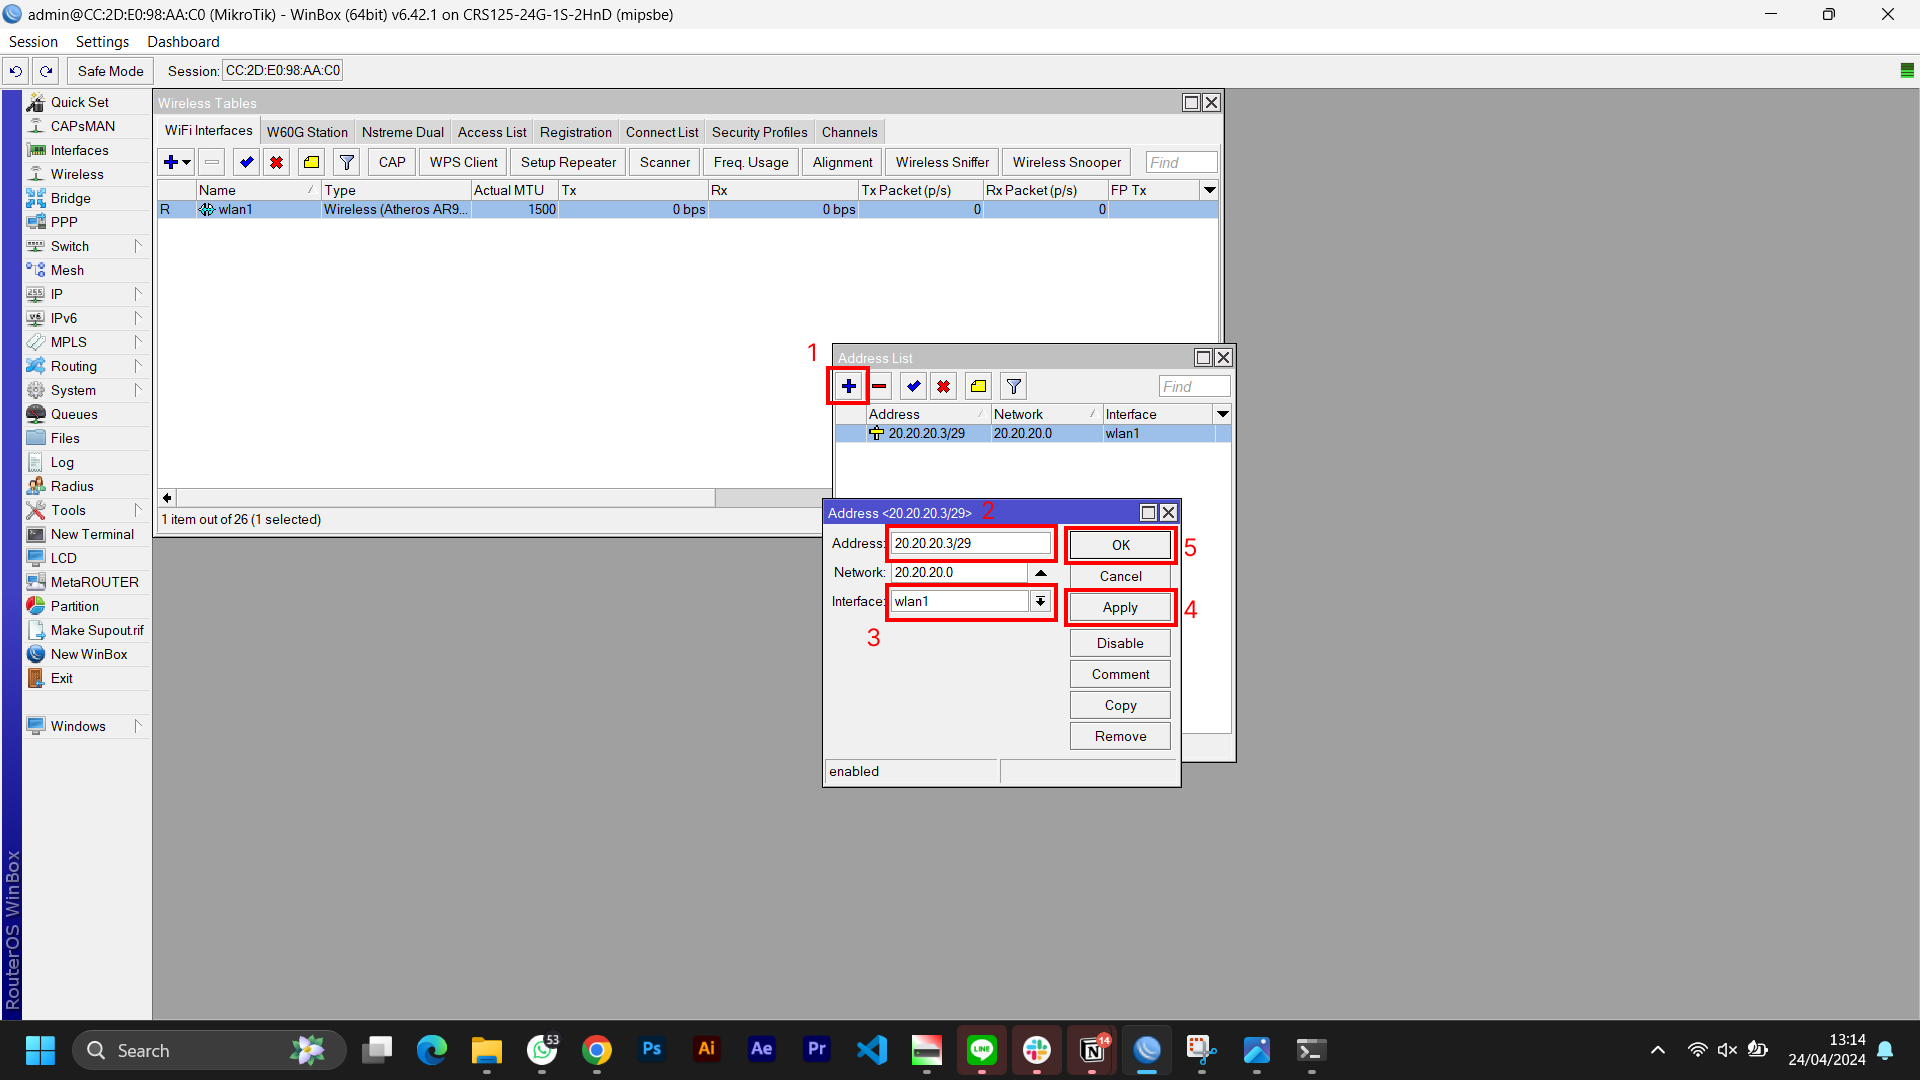
\includegraphics[width=0.9\linewidth]{P1/img/per1/pc2/Step 2.png}
				\caption{Step 2}
				\label{fig:Step 2(Per.1 PC2)}
			\end{figure}
	\end{enumerate}

	\textbf{Pengujian konfigurasi}
	\begin{enumerate}
	\item Lakukan test ping dari Router 1 ke Router 2
	\begin{figure}[H]
		\centering
		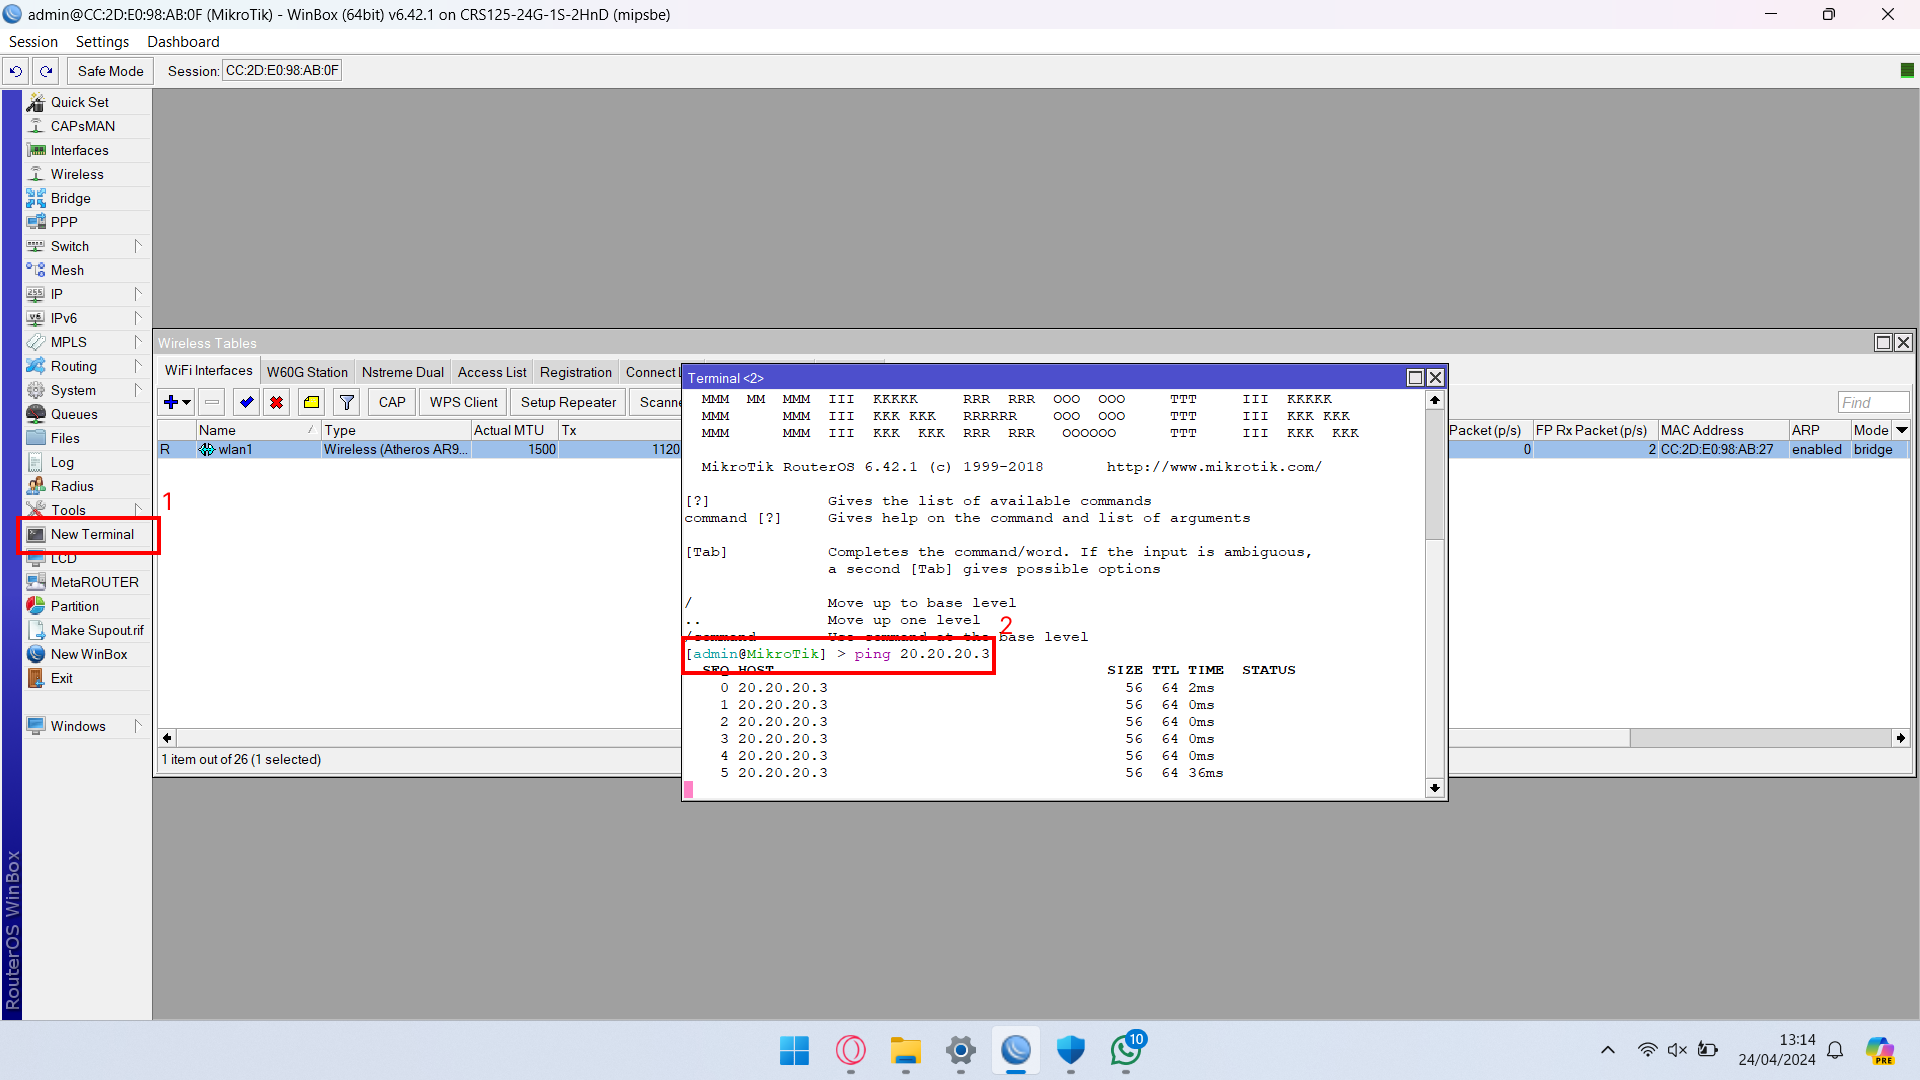
\includegraphics[width=0.9\linewidth]{P1/img/per1/pc1/Step 4.png}
		\caption{Step 1}
		\label{fig:Ping Step 1(Per.1 PC1)}
	\end{figure}
	\end{enumerate}
\end{center}

%======================PERCOBAAN 2==========================%
\subsection{Wireless Point to Multipoint}
\begin{center}

	\textbf{Konfigurasi Router 1}
	\begin{enumerate}
		\item Berikan IP address sesuai dengan cara pengaturan IP address yang benar. Berikan IP address yang berbeda dengan contoh di modul.
		      \begin{figure}[H]
			      \centering
			      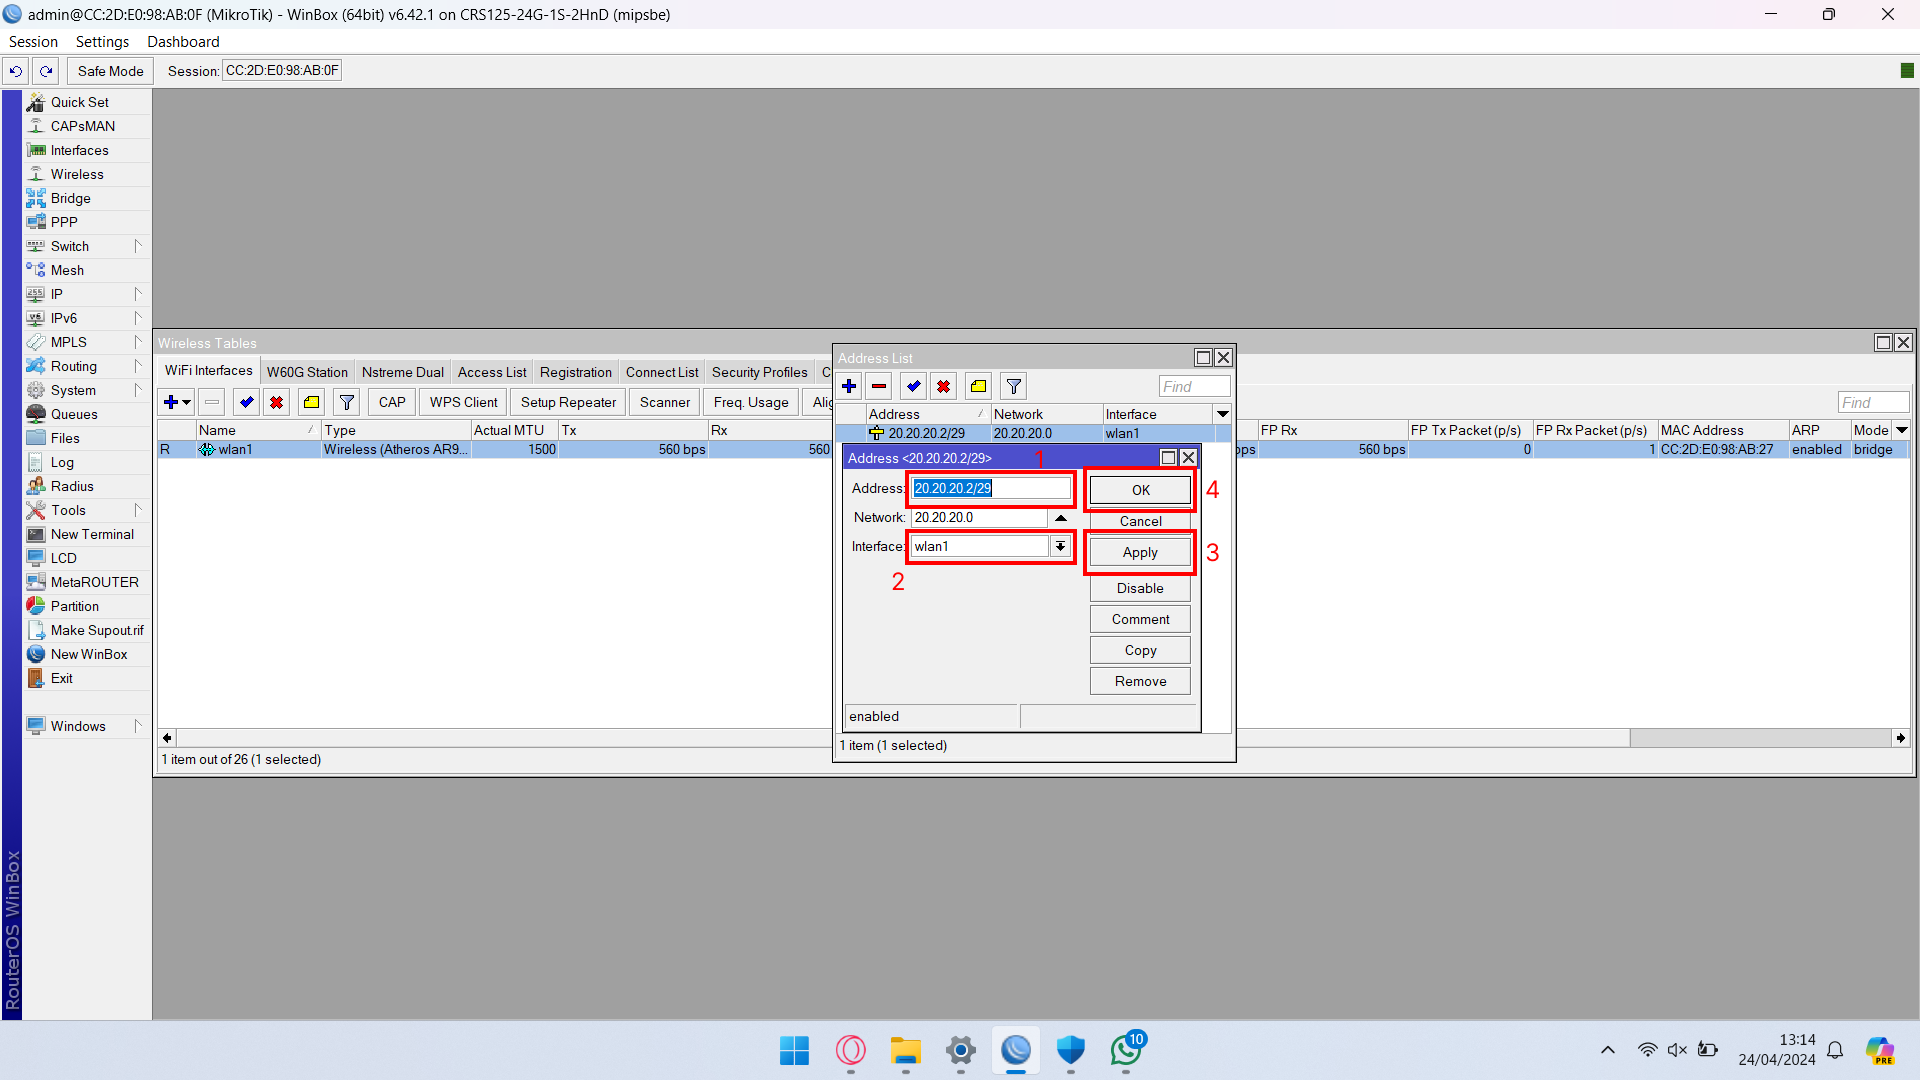
\includegraphics[width=0.9\linewidth]{P1/img/per1/pc1/Step 2.2.png}
			      \caption{Step 1}
			      \label{fig:Step 1(Per.2 PC1)}
		      \end{figure}
	\end{enumerate}

	\textbf{Konfigurasi Router 2}
	\begin{enumerate}
		\item Berikan IP address pada interface wlan 1 yang dapat dibuat pada tab IP > Addresses. Berikan IP address sesuai dengan cara pengaturan IP address yang benar. Berikan IP address yang berbeda dengan contoh di modul.
		      \begin{figure}[H]
			      \centering
			      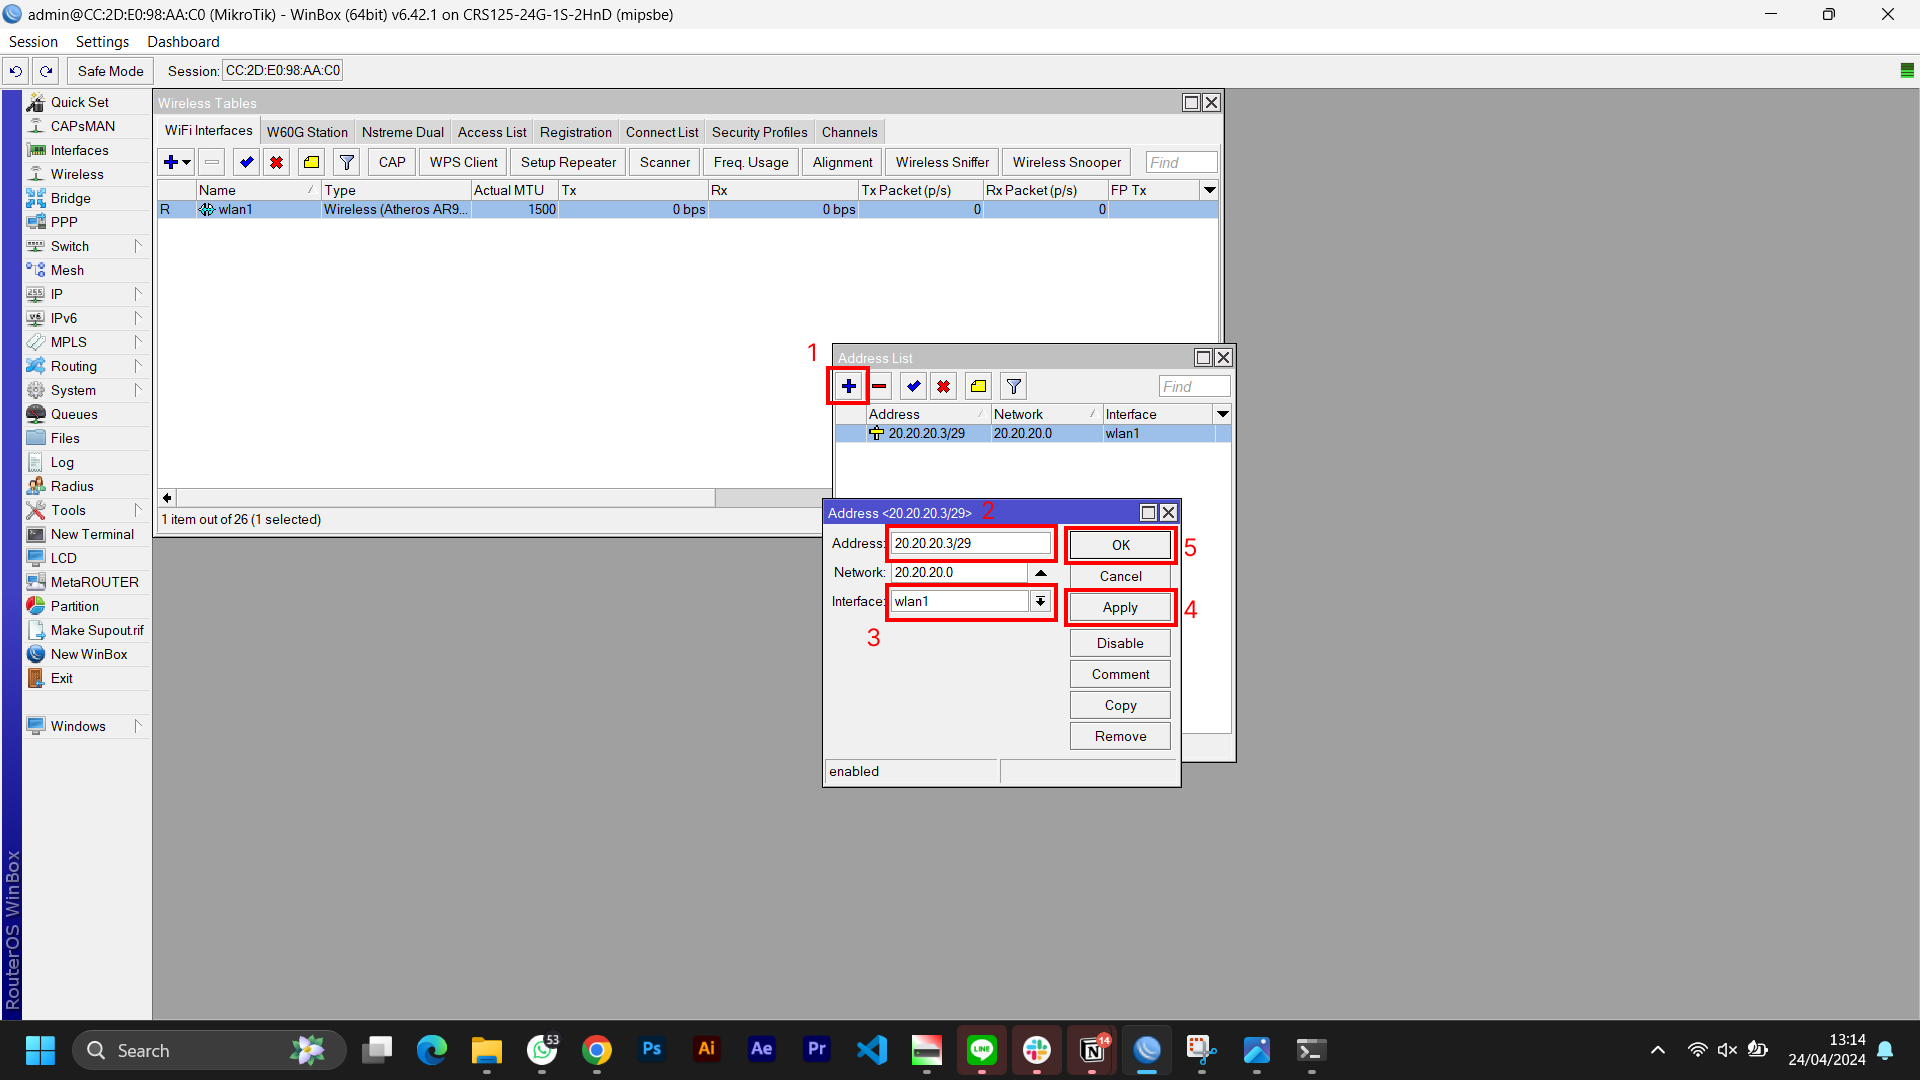
\includegraphics[width=0.9\linewidth]{P1/img/per1/pc2/Step 2.png}
			      \caption{Step 1}
			      \label{fig:Step 1(Per.2 PC2)}
		      \end{figure}
	\end{enumerate}

	\textbf{Pengujian konfigurasi}
	\begin{enumerate}
		\item Lakukan test ping dari Router 1 ke Router 2
		      \begin{figure}[H]
			      \centering
			      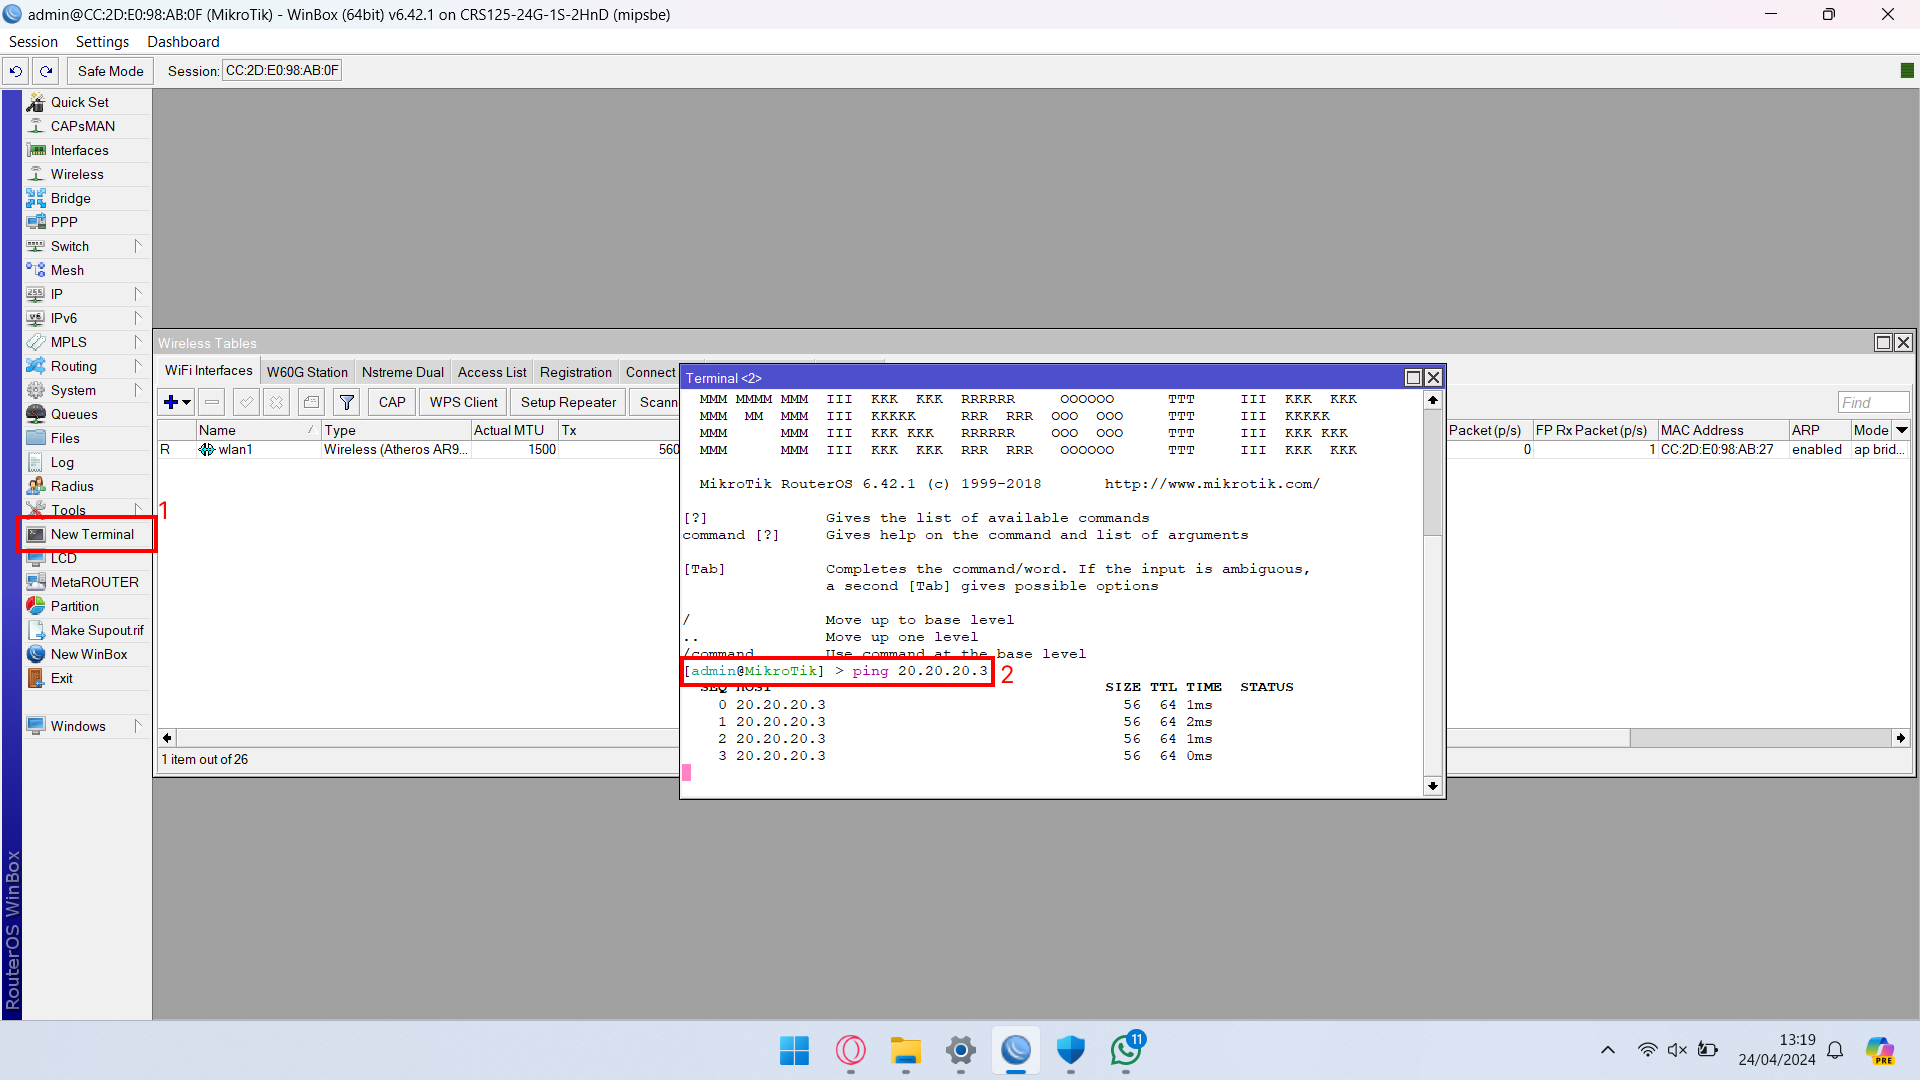
\includegraphics[width=0.9\linewidth]{P1/img/per2/pc1/Step 4.png}
			      \caption{Step 1}
			      \label{fig:Ping Step 1(Per.2 PC1)}
		      \end{figure}
	\end{enumerate}

\end{center}

%======================PERCOBAAN 3==========================%
\subsection{Wireless Bridge}
\begin{center}

	\textbf{Konfigurasi Router 1}
	\begin{enumerate}
		\item Buka WinBox dan lakukan koneksi ke Router
		      \begin{figure}[H]
			      \centering
			      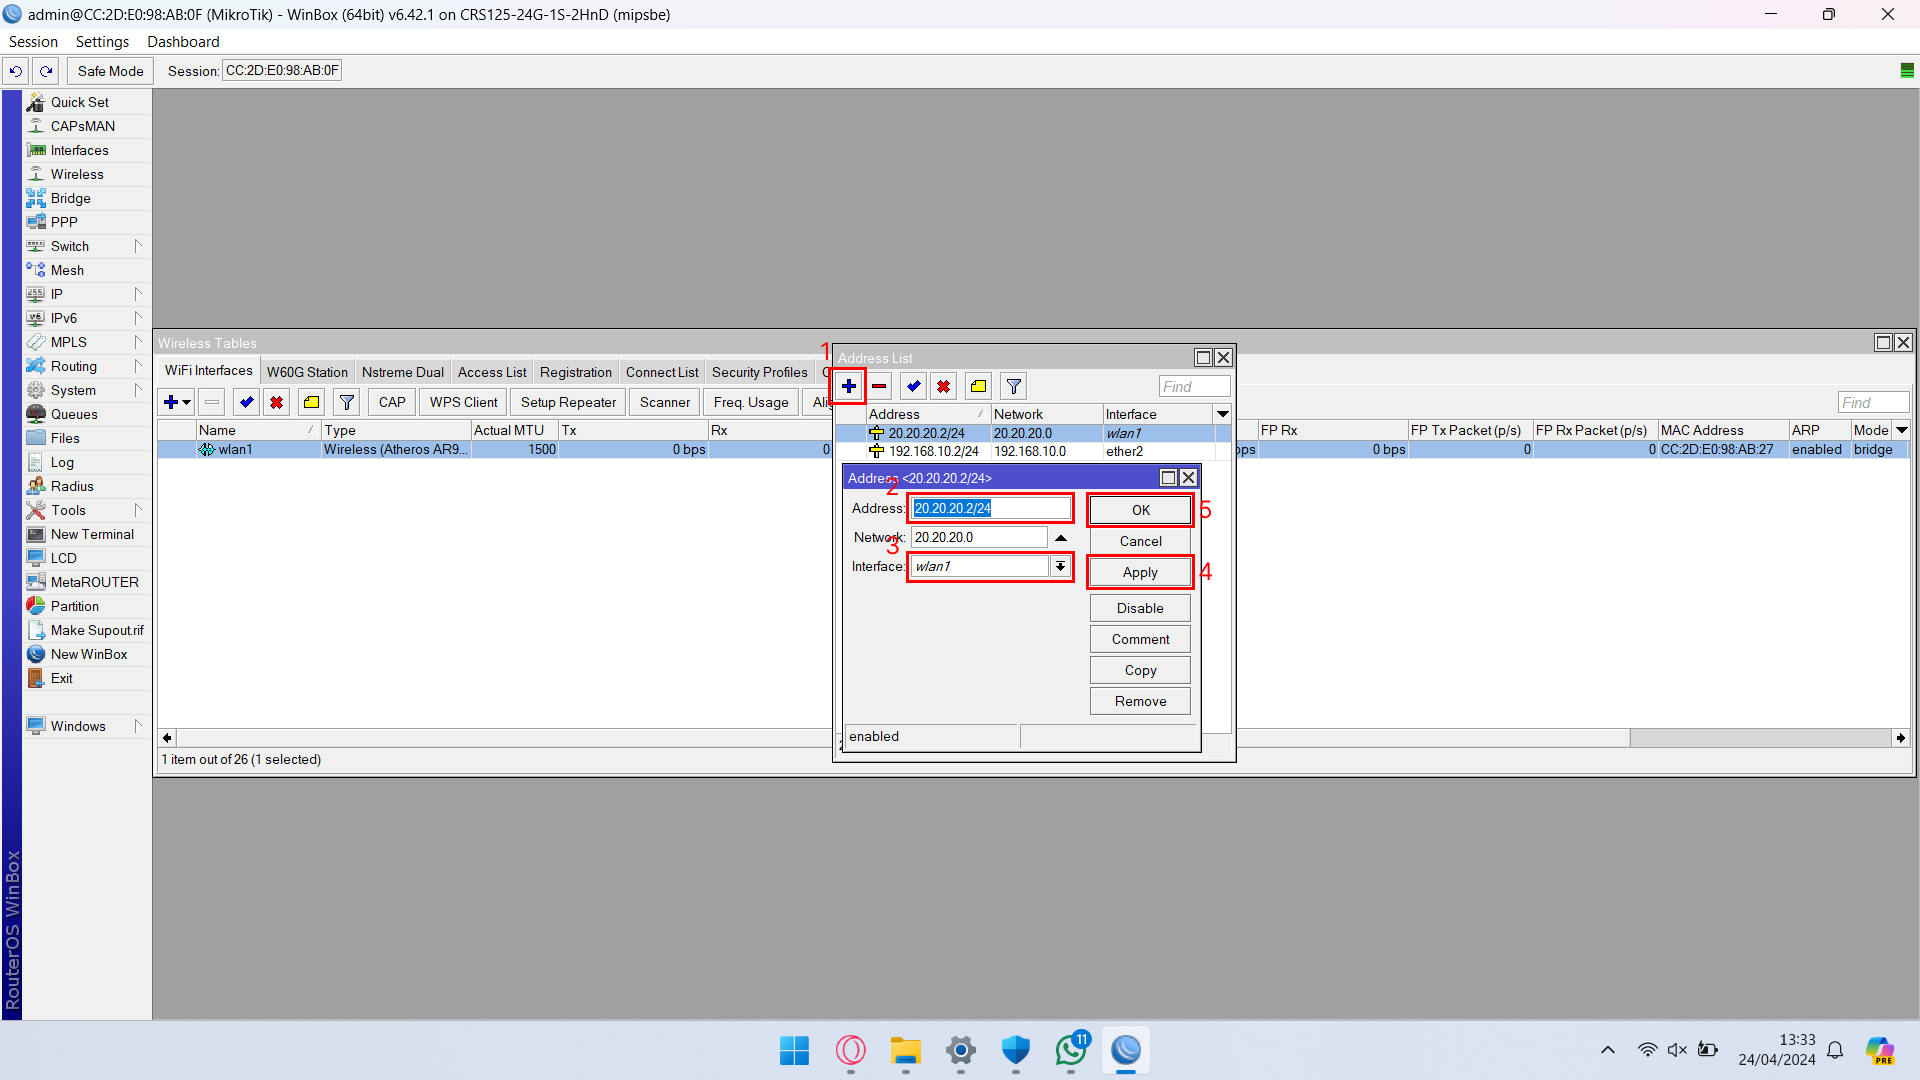
\includegraphics[width=0.9\linewidth]{P1/img/per3/pc1/Step 2.png}
			      \caption{Step 2}
			      \label{fig:Step 2(Per.3 PC1)}
		      \end{figure}
	\end{enumerate}

	\textbf{Konfigurasi Router 2}
	\begin{enumerate}
		\item Berikan IP address pada interface wlan1 dan ethernet 2 yang dapat dibuat pada tab IP > Addresses. Berikan IP address sesuai dengan cara pengaturan IP address yang benar. Berikan IP address yang berbeda dengan contoh di modul.
		      \begin{figure}[H]
			      \centering
			      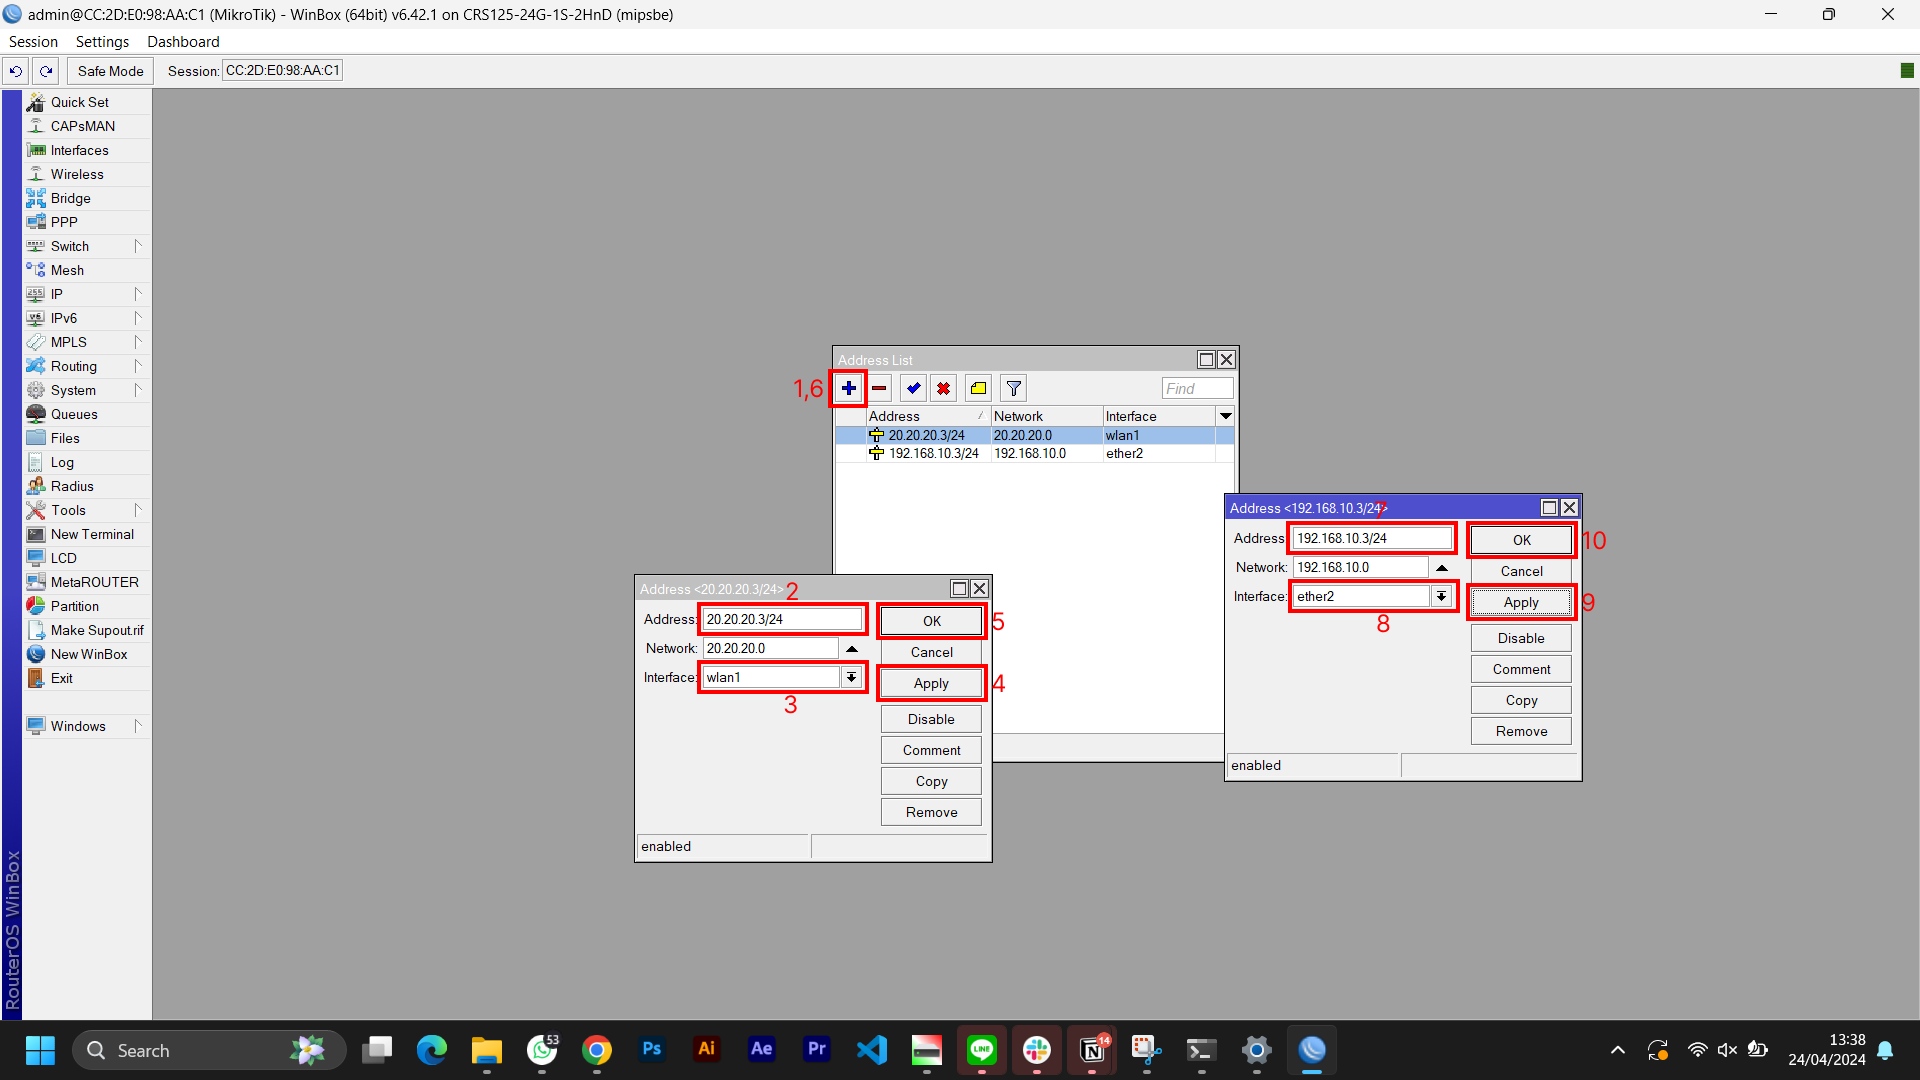
\includegraphics[width=0.9\linewidth]{P1/img/per3/pc2/Step 2.png}
			      \caption{Step 2}
			      \label{fig:Step 2(Per.3 PC2)}
		      \end{figure}
	\end{enumerate}

	\textbf{Pengujian konfigurasi}
	\begin{enumerate}
		\item Lakukan test ping dari PC 1 ke PC 2
		      \begin{figure}[H]
			      \centering
			      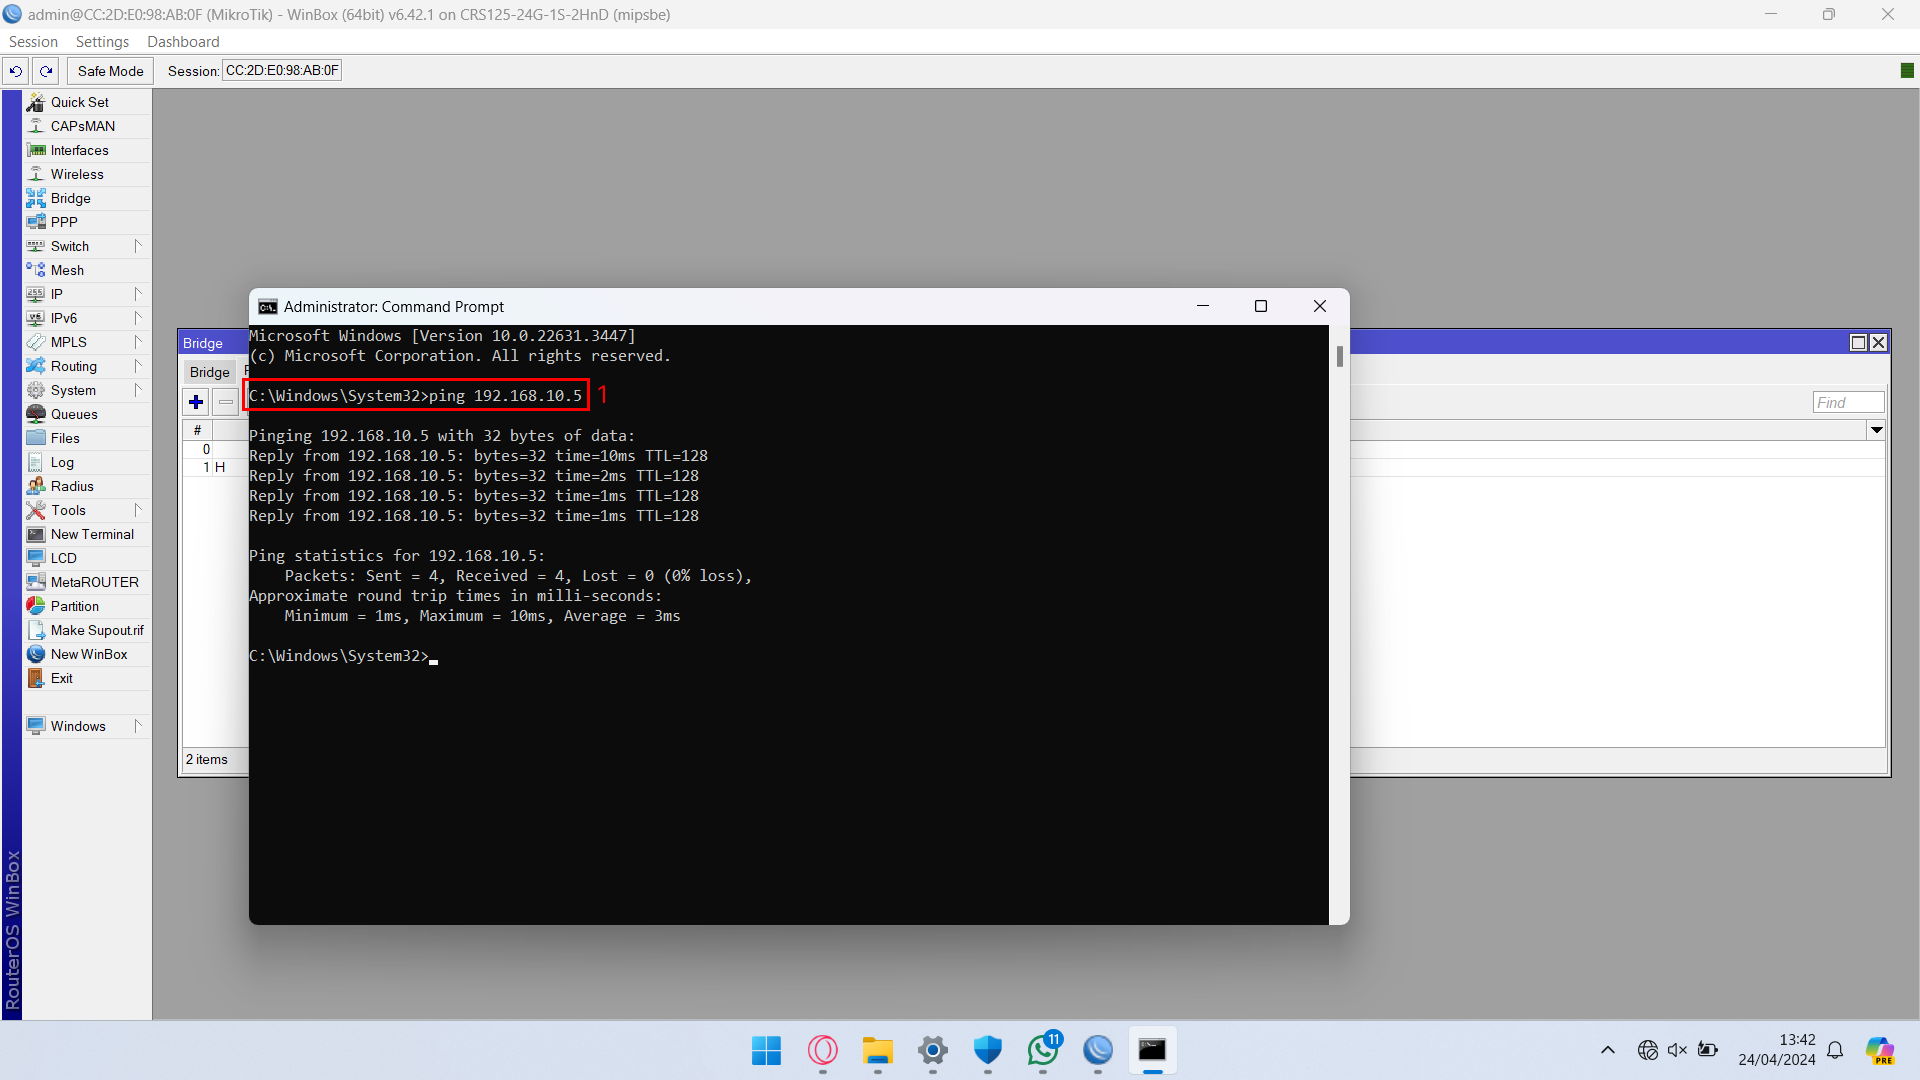
\includegraphics[width=0.9\linewidth]{P1/img/per3/pc1/Step 7.png}
			      \caption{Step 7}
			      \label{fig:Step 7(Per.3 PC1)}
		      \end{figure}
	\end{enumerate}

\end{center}

%===========================================================%
\section{Hasil yang didapat}
Memahami dan mengkonfigurasi koneksi Point to Point, Point to Multipoint dan Wireless
Bridging dengan tepat.

%===========================================================%
\section{Temuan Permasalahan}
Firewall hidup pada Laptop dapat mempengaruhi koneksi wireless tidak terhubung, kalian
bisa menonaktifkan firewall di laptop kalian, tetapi hal ini tidak terjadi di semua perangkat.

%===========================================================%
\section{Kesimpulan}
Dengan memahami dan mengkonfigurasi 3 jenis koneksi pada wireless, kita dapat
mengimplementasikan koneksi wireless dengan tepat sesuai kebutuhan dan kondisi tertentu.

% \section{Pendahuluan}
\subsection{Latar Belakang}
Pada modul kedua ini, kita akan membahas perbandingan hasil (ADC) analog to digital converter pada Arduino dan Osiloskop.Analog to Digital Converter (ADC) adalah perangkat yang berfungsi untuk mengubah sinyal analog menjadi sinyal digital. 
Sinyal analog adalah sinyal yang memiliki nilai yang berubah-ubah dalam waktu, sedangkan sinyal digital adalah sinyal yang memiliki nilai yang berubah-ubah dalam waktu tetapi hanya memiliki dua nilai, yaitu 0 dan 1.
\\\\
ADC umumnya menggunakan metode Successive Approximation Register (SAR) atau metode lainnya untuk mengkonversi sinyal analog menjadi sinyal digital. 
Misalnya, pada Arduino, ADC menggunakan metode SAR untuk mengkonversi tegangan analog menjadi nilai digital yang dapat diproses oleh mikrokontroler.
\\\\
Pada modul praktikum, praktikan menggunakan Arduino untuk membaca tegangan analog dan mengkonversinya menjadi nilai digital menggunakan ADC. 
Sementara itu, osiloskop digunakan untuk memvisualisasikan sinyal listrik dan membandingkan hasil konversi ADC dengan sinyal aslinya.
\\\\

\subsection{Maksud dan Tujuan}
Mengetahui dan membandingkan hasil dari analog to digital converter pada Arduino dan Osiloskop.

\subsection{Hasil yang diharapkan}
Mendapatkan kesimpulan perbandingan hasil analog to digital converter pada Arduino dan Osiloskop.
%===========================================================%
\section{Tugas Pendahuluan}


\begin{center}
	\colorbox{cyan!30}{\parbox{0.8\linewidth}{
		\begin{enumerate}
		\item Buatlah topologi jaringan percobaan 1, 2, dan 3!
		\item Perbedaan Static Routing dan Dynamic Routing.
		\item Keuntungan dan kekurangan Static Routing dan Dynamic Routing
	\end{enumerate}
	}}
\end{center}

%===========================================================%
\section{Alat dan Bahan}
\begin{itemize}[label=$\bullet$, itemsep=-1pt, leftmargin=*]
	\item 2 perangkat router mikrotik.
	\item Aplikasi Winbox.
	\item 3 kabel LAN
\end{itemize}

%===========================================================%
\section{Jangka Waktu Pelaksanaan}
Pemahaman dan konfigurasi 1 jam.

%===========================================================%
\section{Penjelasan dan Tahapan Konfigurasi}

%======================PERCOBAAN 1==========================%
\subsection{Routing Statis}
Pada routing statis, terdapat setidaknya 2 jenis, yaitu
\begin{enumerate}
	\item Default Route : digunakan ketika tidak ada rute spesifik yang cocok untuk tujuan pengiriman data. Jika tidak ada rute yang cocok, paket data akan dikirim melalui default route. Pada MikroTik, default route dinyatakan sebagai 0.0.0.0/0.
	\item Static Route : adalah jenis routing di mana administrator jaringan secara manual mengonfigurasi tabel routing pada setiap perangkat jaringan. Dalam routing static, rute yang ditentukan secara manual digunakan untuk mengarahkan paket data ke tujuan yang ditentukan.
\end{enumerate}

\begin{center}
	\textbf{Konfigurasi Router 1}
	\begin{enumerate}
		\item Buka aplikasi WinBox pada PC 1 dan lakukan koneksi ke Router 1. Neighbors > Refresh > Double click Router yang terdeteksi > Connect
		\begin{figure}[H]
			\centering
			\includegraphics[width=0.8\linewidth]{P2/img/per1/pc1/Step 1.png}
			\caption{Step 1}
			\label{fig:Step 1(Per.1 PC1)}
		\end{figure}
		\item Berikan IP address pada interface ether2 dan ether 4 yang dapat dibuat pada tab IP > Addresses. Berikan IP address sesuai dengan cara pengaturan IP address yang benar. Berikan IP address yang berbeda dengan contoh di modul.
		\begin{figure}[H]
			\centering
			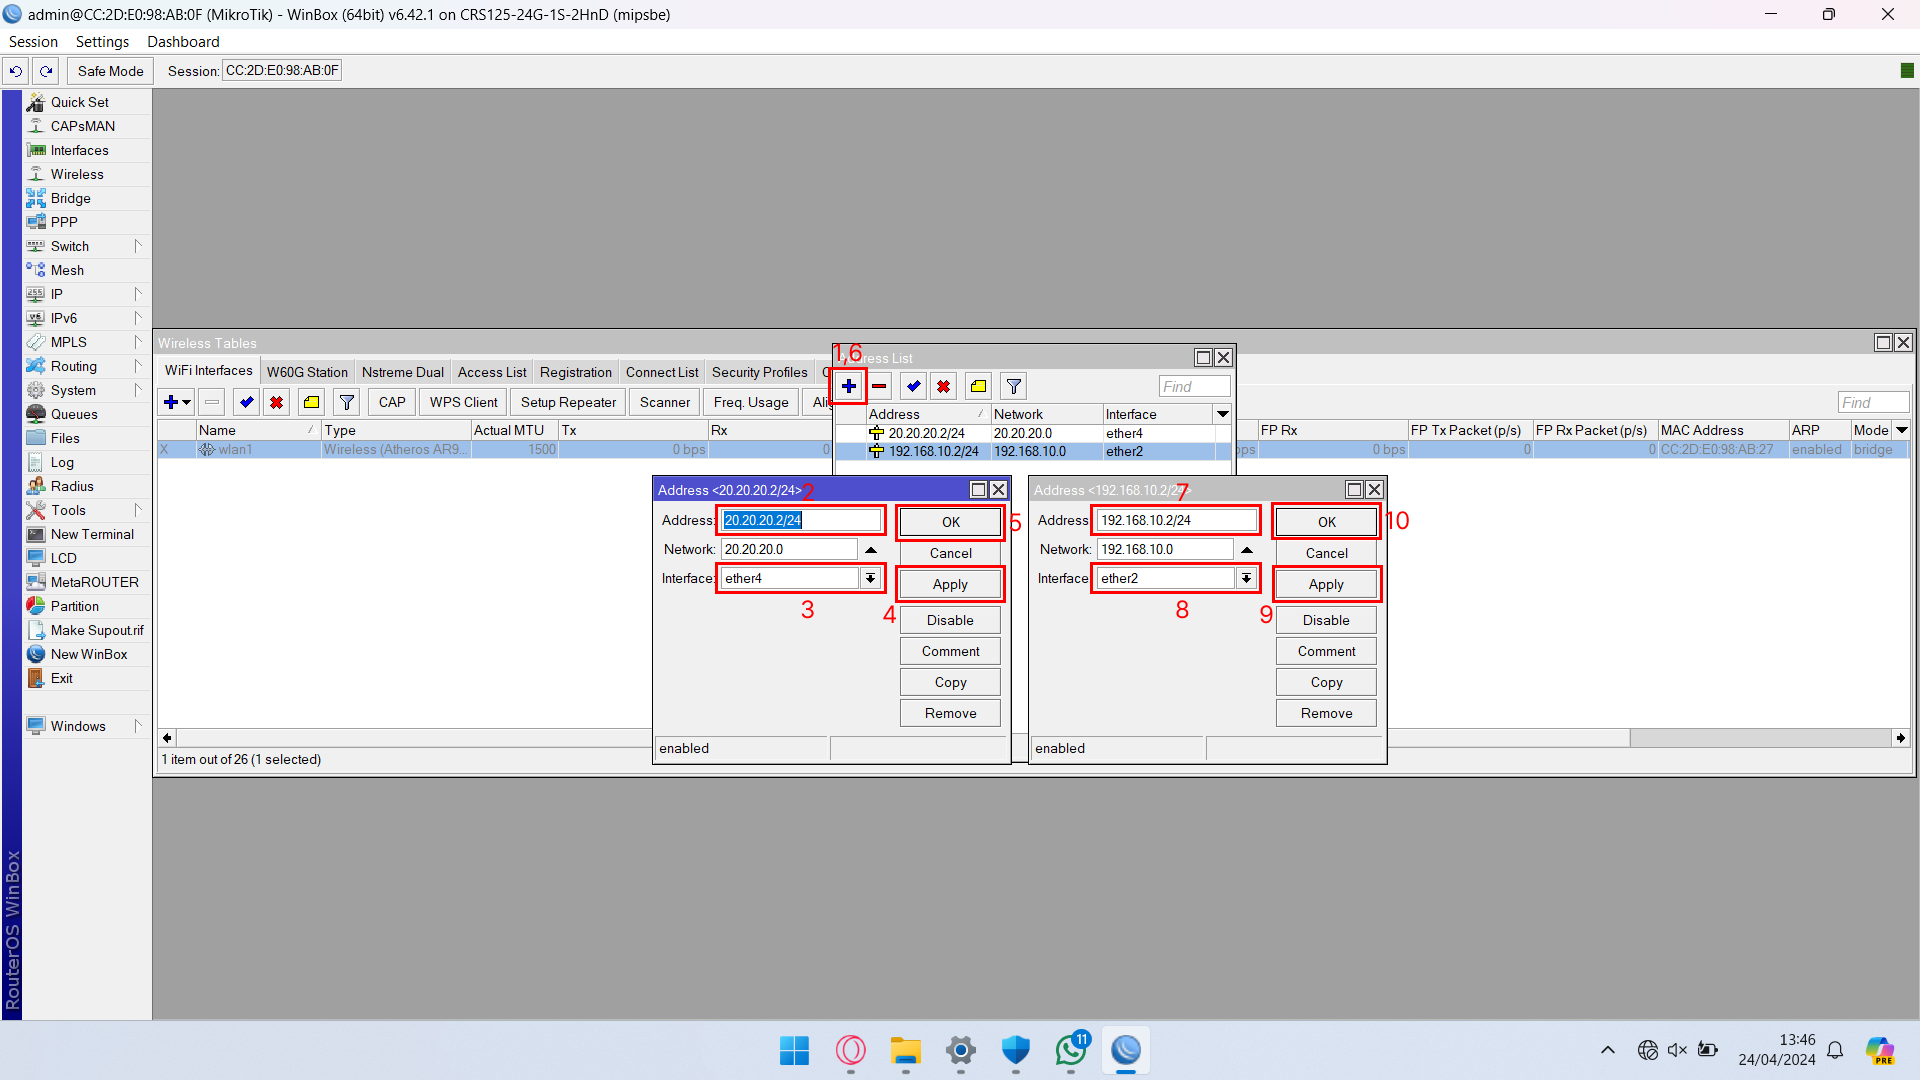
\includegraphics[width=0.9\linewidth]{P2/img/per1/pc1/Step 2.png}
			\caption{Step 2}
			\label{fig:Step 2(Per.1 PC1)}
		\end{figure}
		\item Lakukan routing statis. Buka pada tab IP > Routes, lalu tambahkan jaringan. 
		\begin{figure}[H]
			\centering
			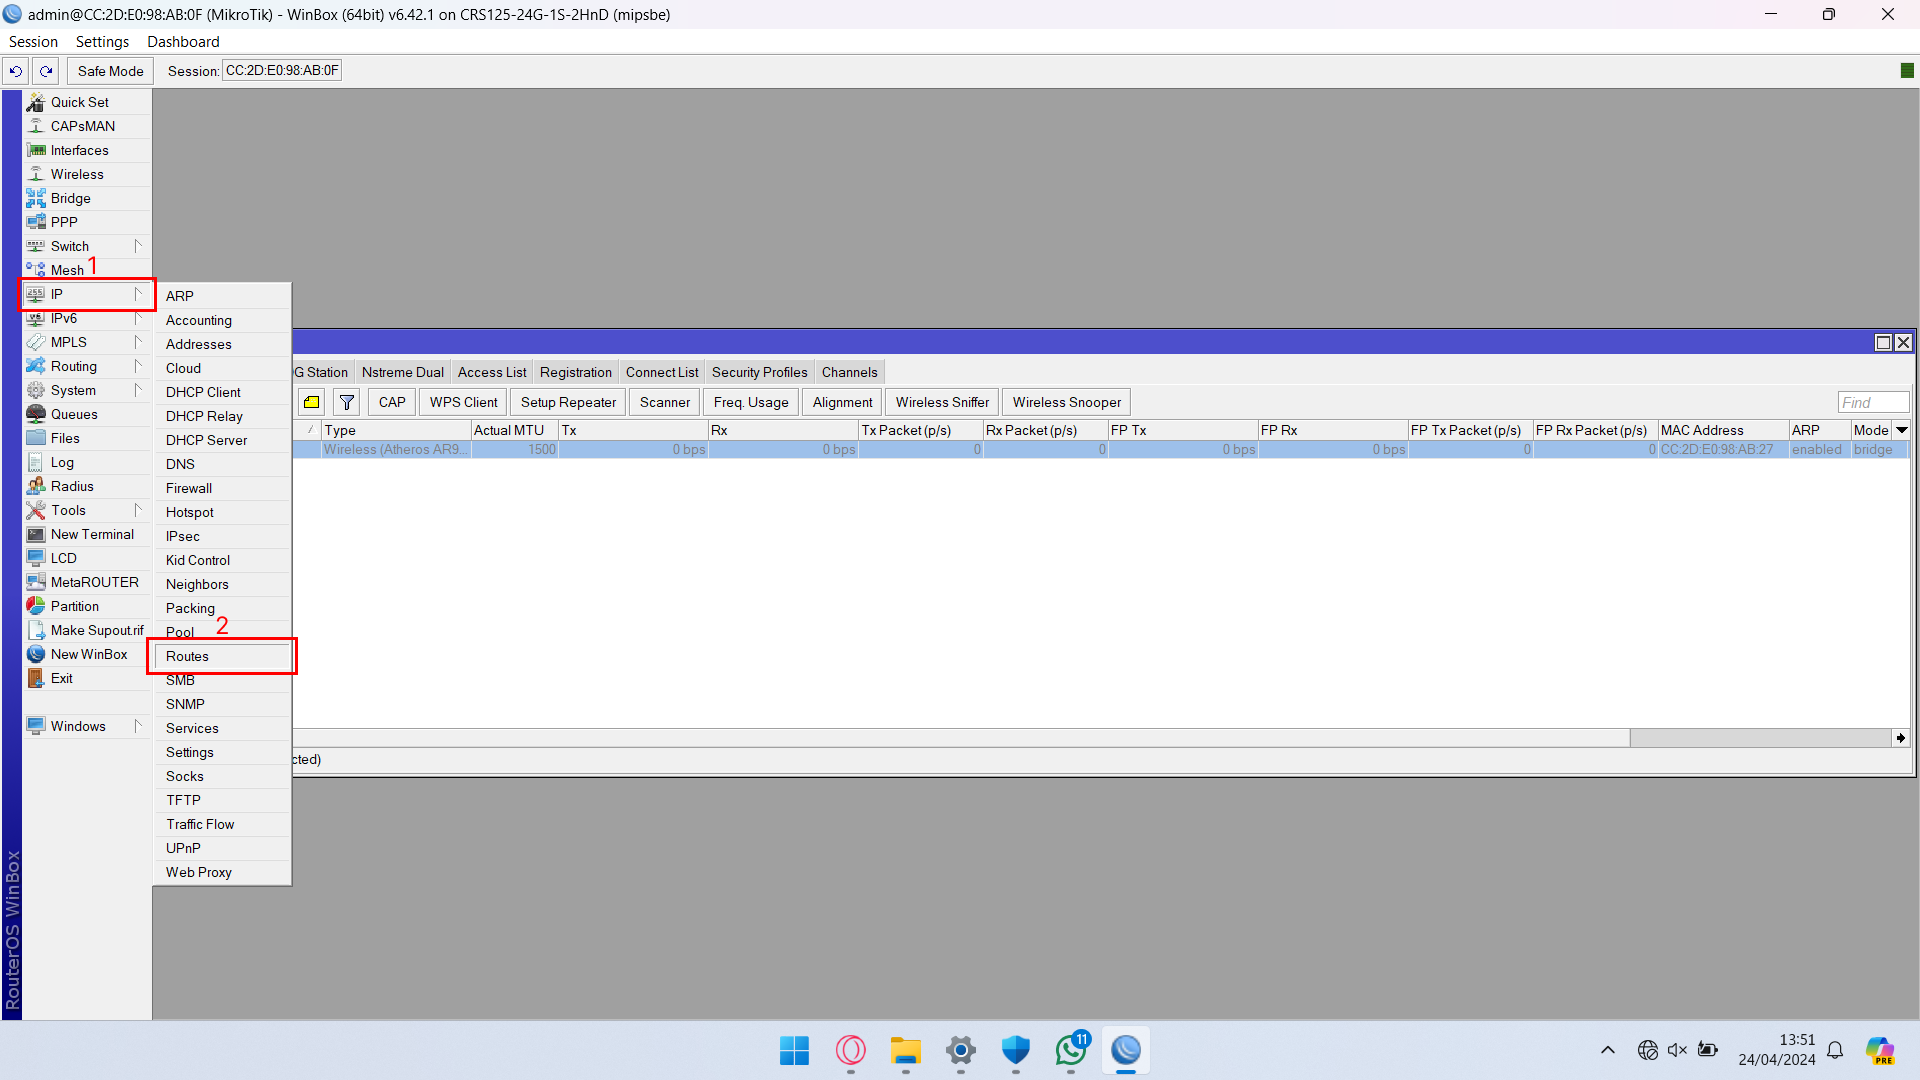
\includegraphics[width=0.9\linewidth]{P2/img/per1/pc1/Step 3.1.png}
			\caption{Step 3.1}
			\label{fig:Step 3.1(Per.1 PC1)}
		\end{figure}
		Masukkan alamat jaringan yang ingin dituju, melalui alamat Gateway pada router 2
		\begin{figure}[H]
			\centering
			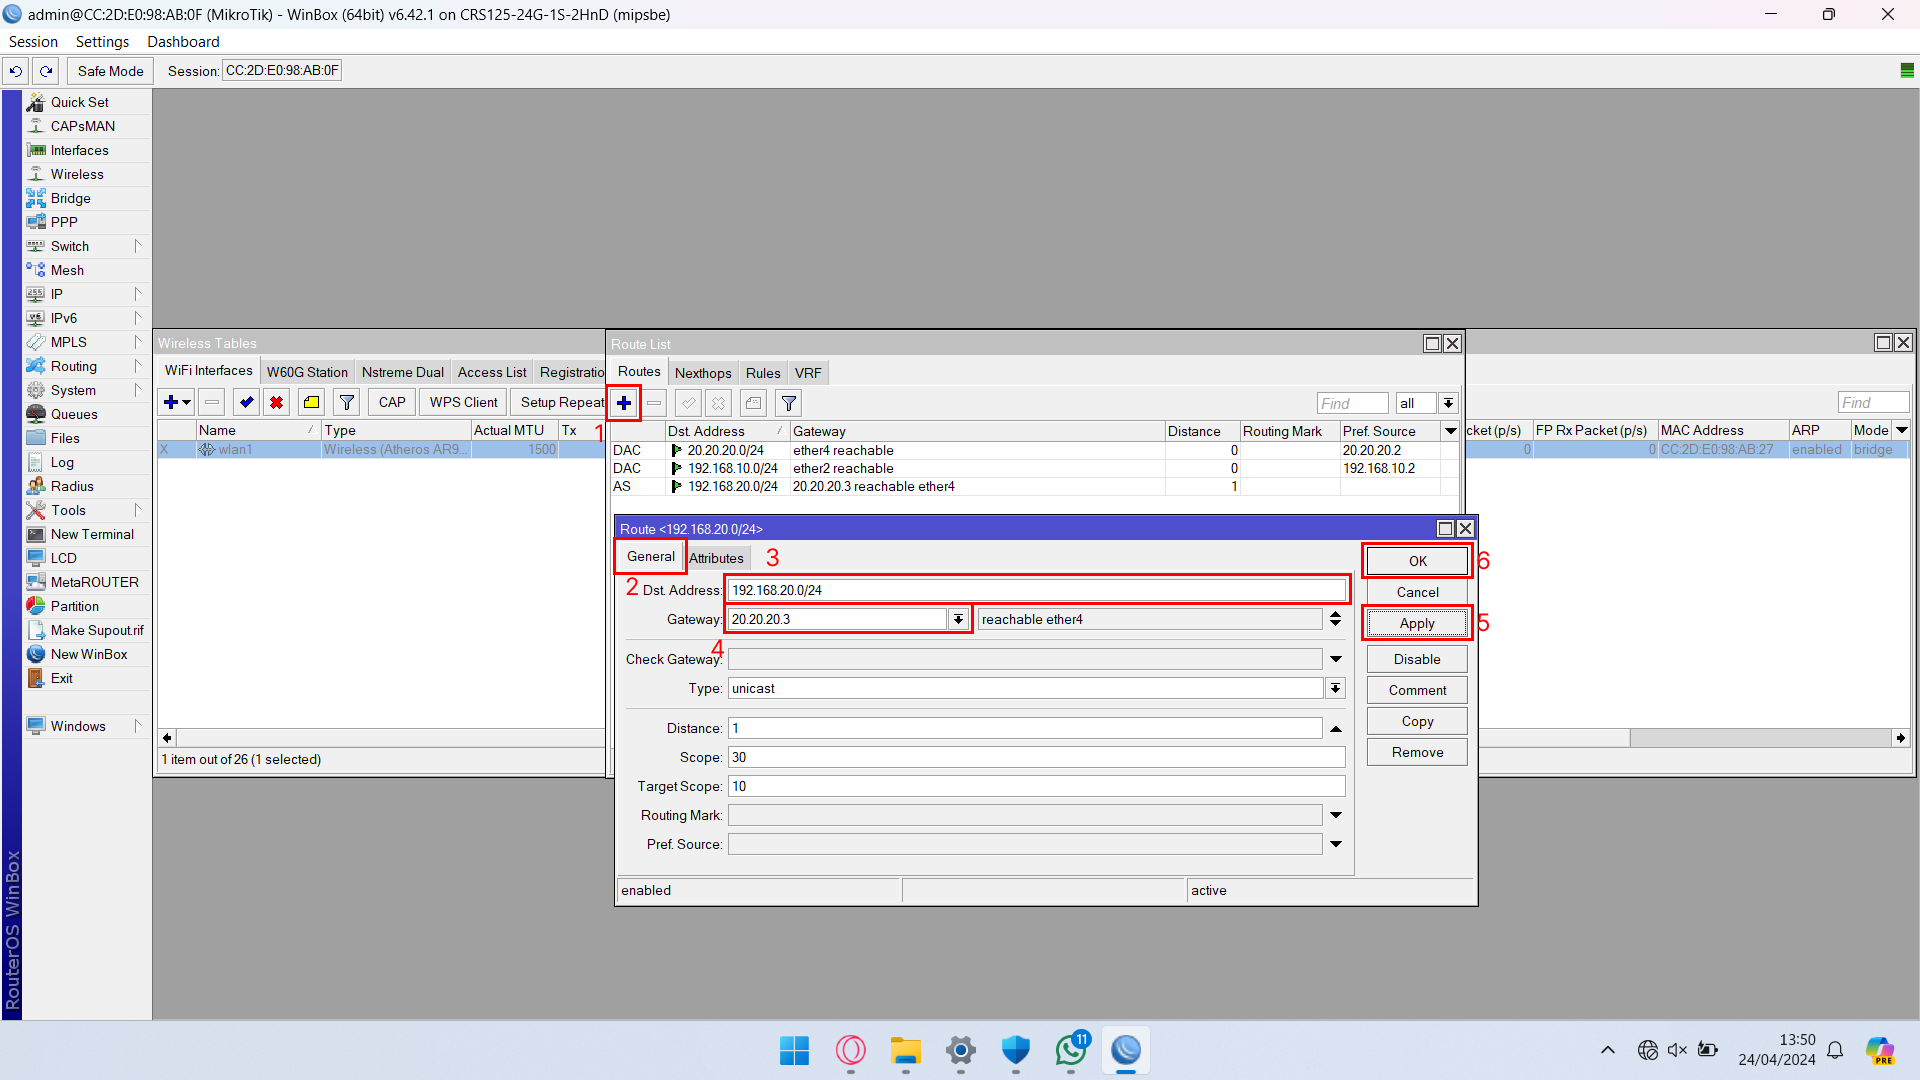
\includegraphics[width=0.9\linewidth]{P2/img/per1/pc1/Step 3.2.png}
			\caption{Step 3.2}
			\label{fig:Step 3.2(Per.1 PC1)}
		\end{figure}
	\end{enumerate}

	\textbf{Konfigurasi Router 2}
	\begin{enumerate}
		\item Buka WinBox dan lakukan koneksi ke Router 2
		\item Berikan IP address pada interface ether2 dan ether 4 yang dapat dibuat pada tab IP > Addresses. Berikan IP address sesuai dengan cara pengaturan IP address yang benar. Berikan IP address yang berbeda dengan contoh di modul.
		\begin{figure}[H]
			\centering
			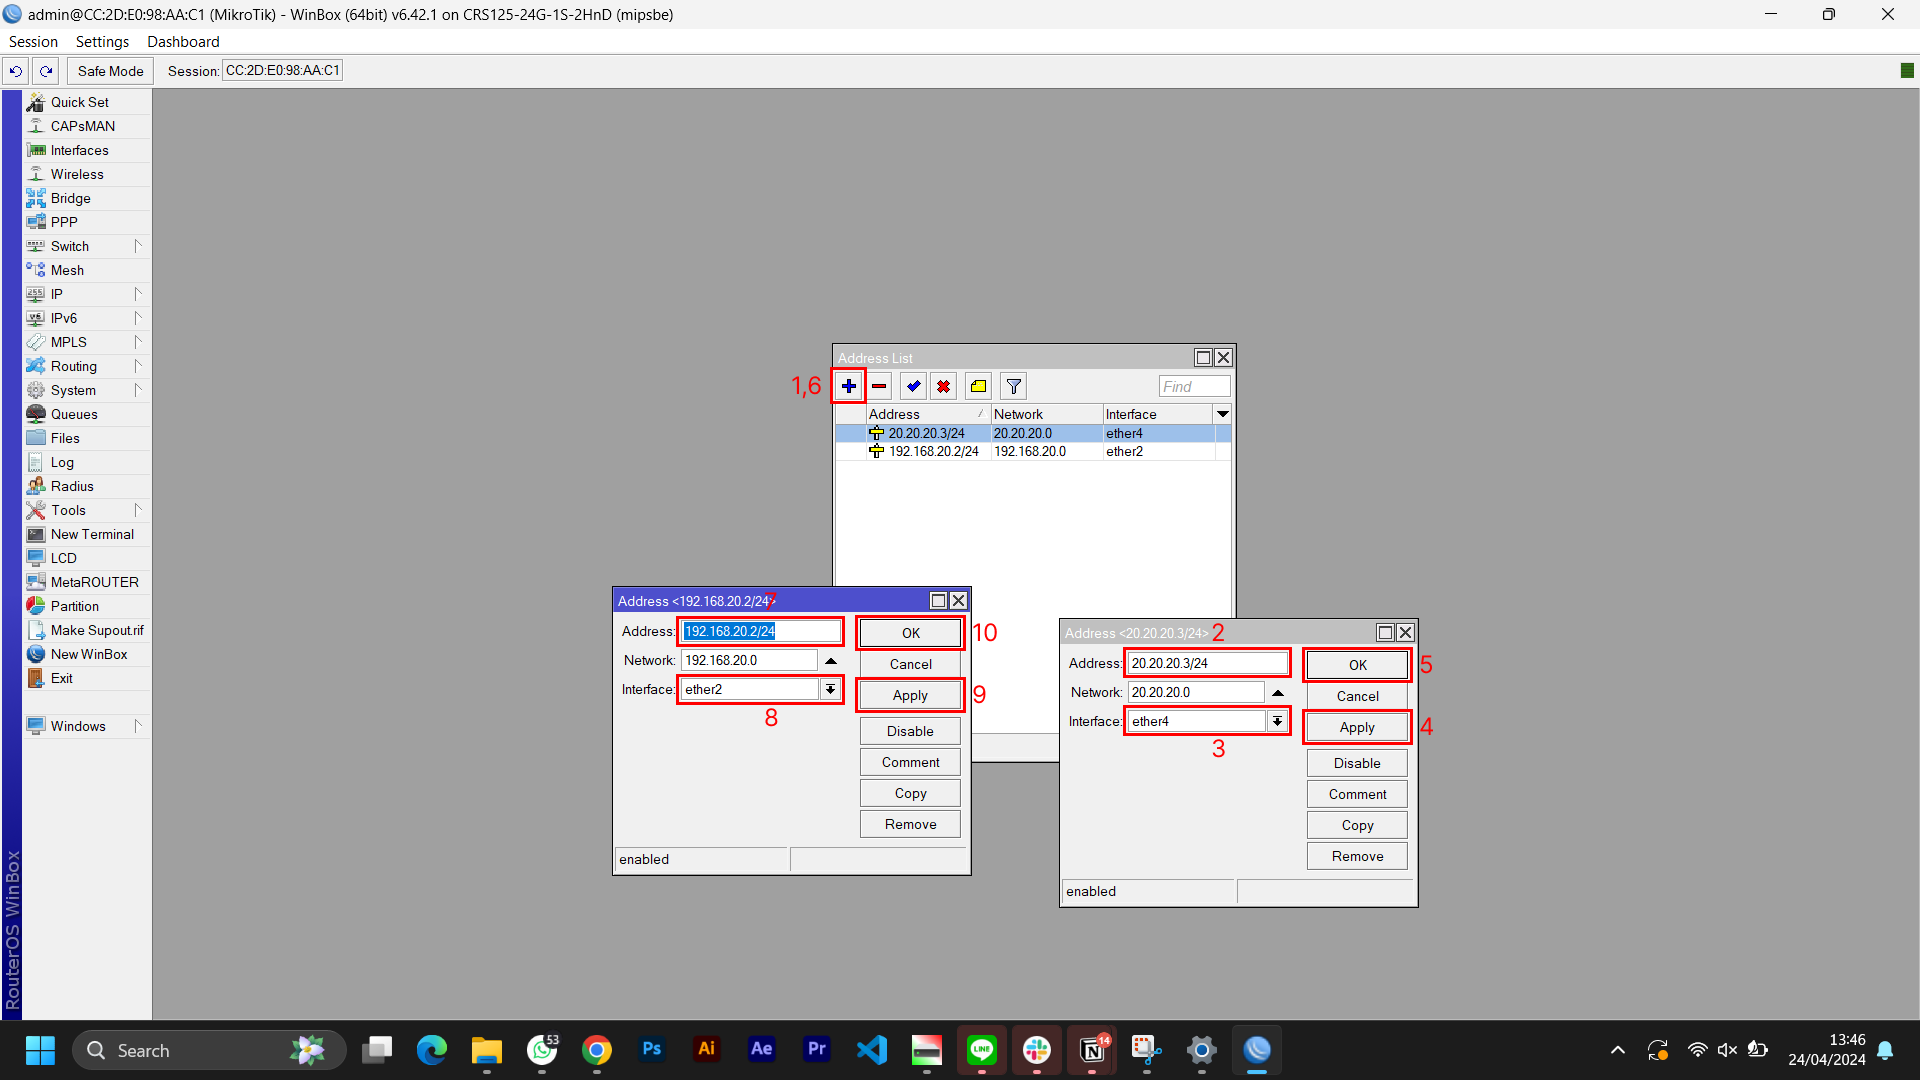
\includegraphics[width=0.9\linewidth]{P2/img/per1/pc2/Step 2.png}
			\caption{Step 2}
			\label{fig:Step 2(Per.1 PC2)}
		\end{figure}
		\item Lakukan routing statis. Buka pada tab IP > Routes, lalu tambahkan jaringan. Masukkan alamat jaringan yang ingin dituju, melalui alamat Gateway pada router 1
		\begin{figure}[H]
			\centering
			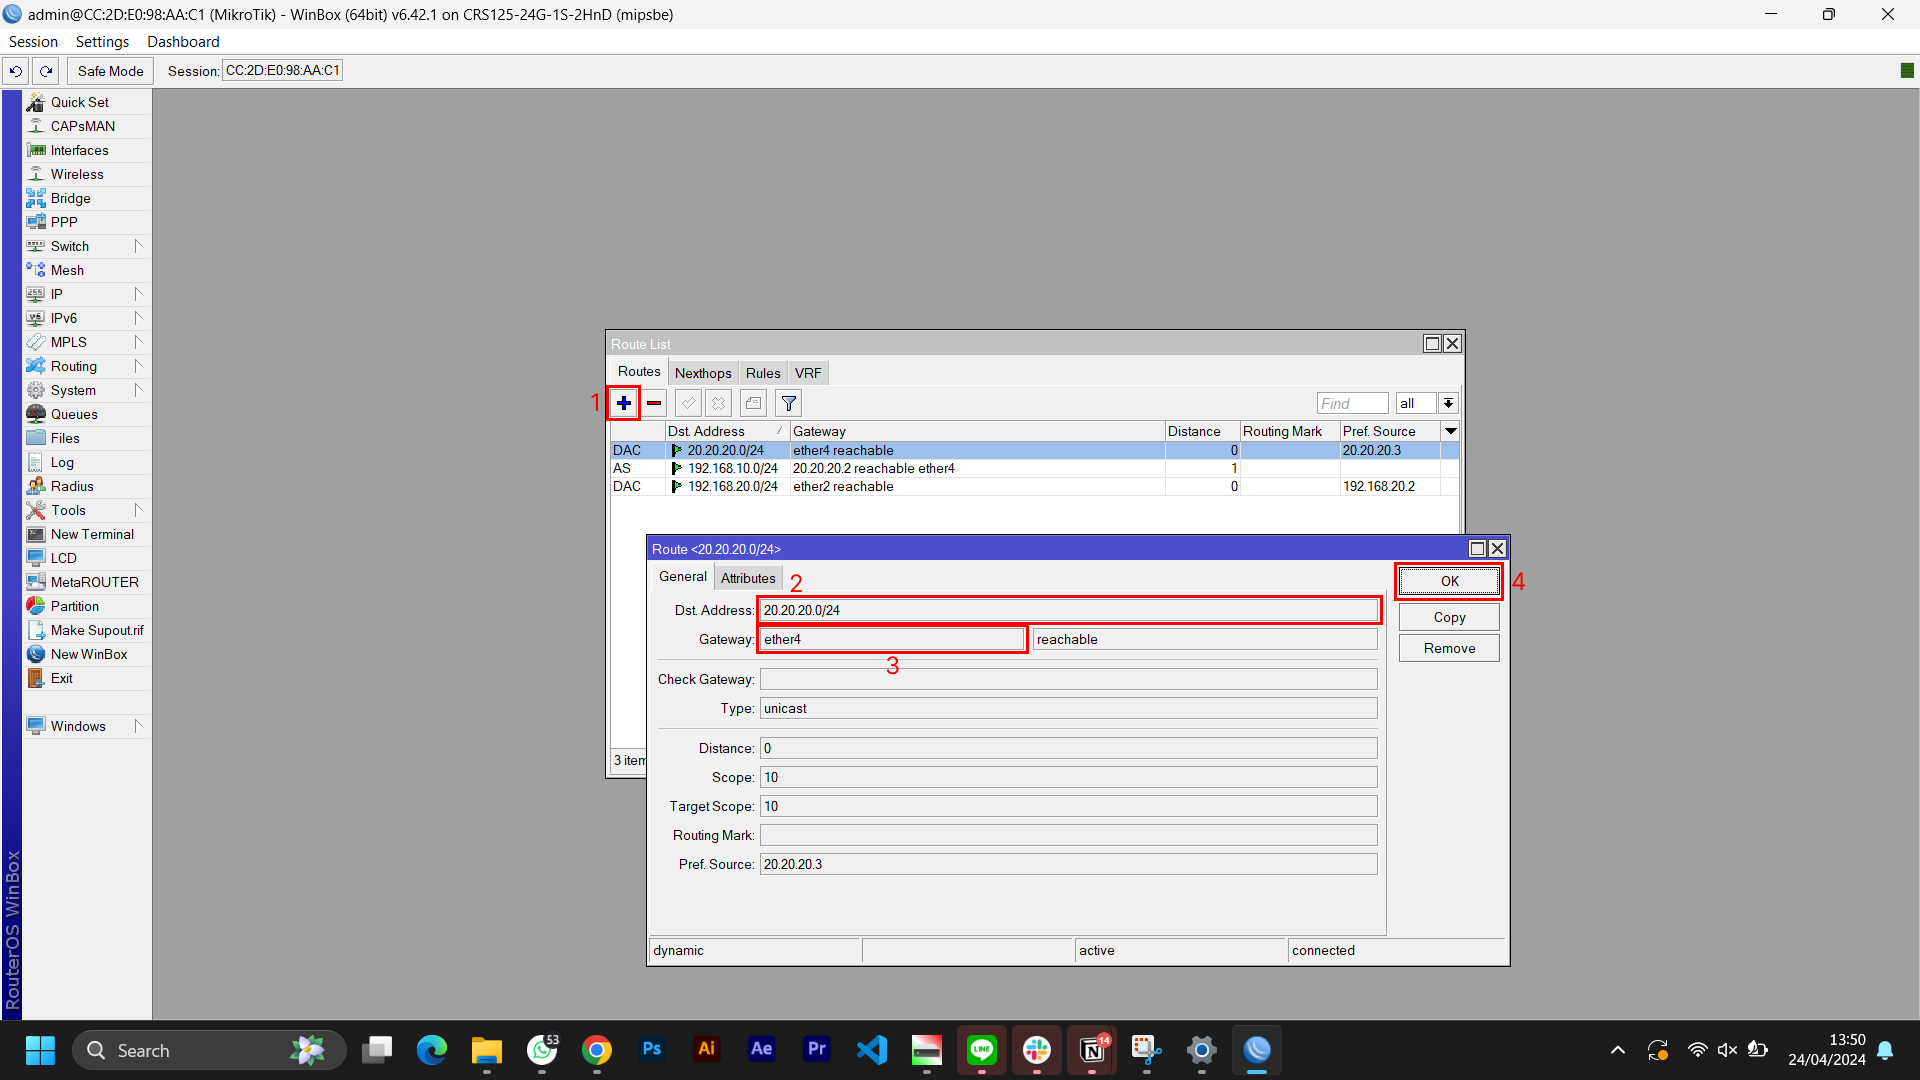
\includegraphics[width=0.9\linewidth]{P2/img/per1/pc2/Step 3.png}
			\caption{Step 3}
			\label{fig:Step 3(Per.1 PC2)}
		\end{figure}
	\end{enumerate}

	\textbf{Pengujian konfigurasi}
	\begin{enumerate}
		\item Lakukan tes ping ke Router 2 melalui Router 1
		\begin{figure}[H]
			\centering
			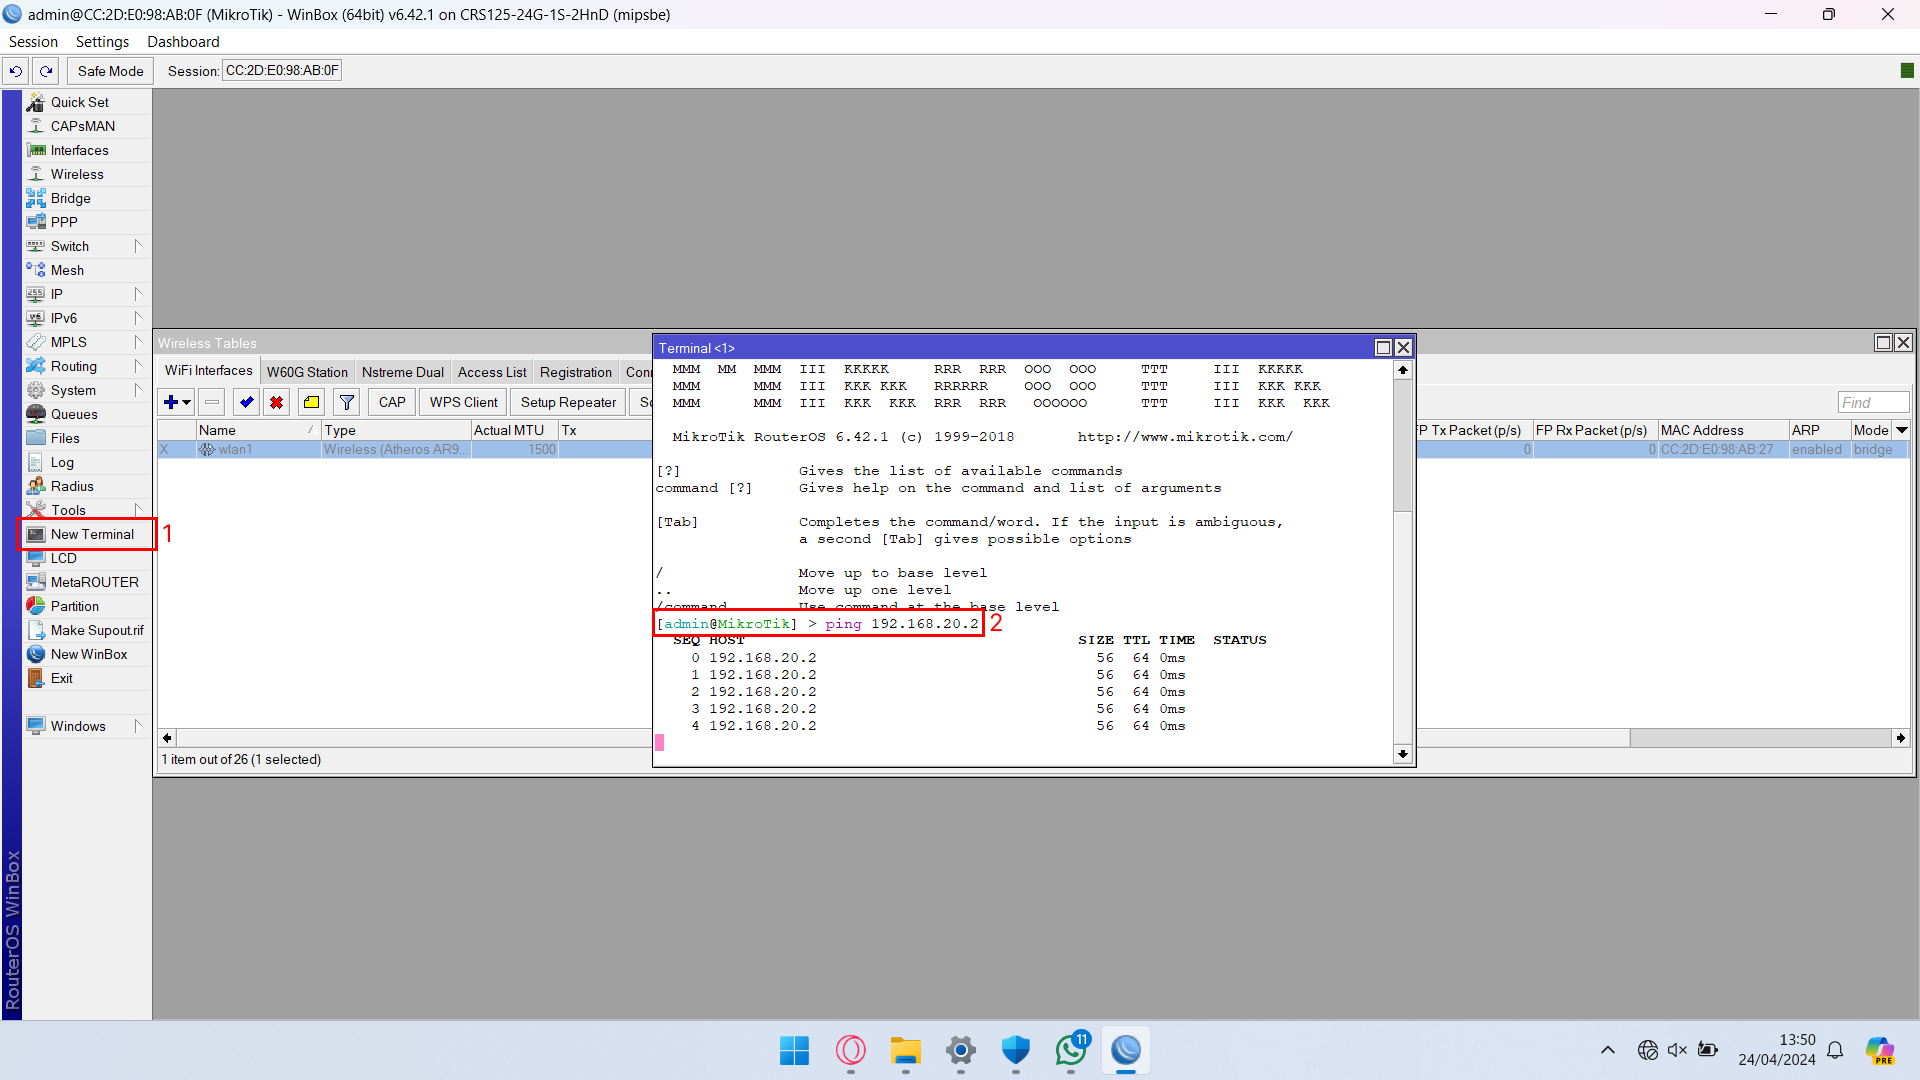
\includegraphics[width=0.9\linewidth]{P2/img/per1/pc1/Step 4.png}
			\caption{Step 1}
			\label{fig:Ping Step 1(Per.1 PC1)}
		\end{figure}
		\item Lakukan tes ping ke Router 1 melalui Router 2
		\begin{figure}[H]
			\centering
			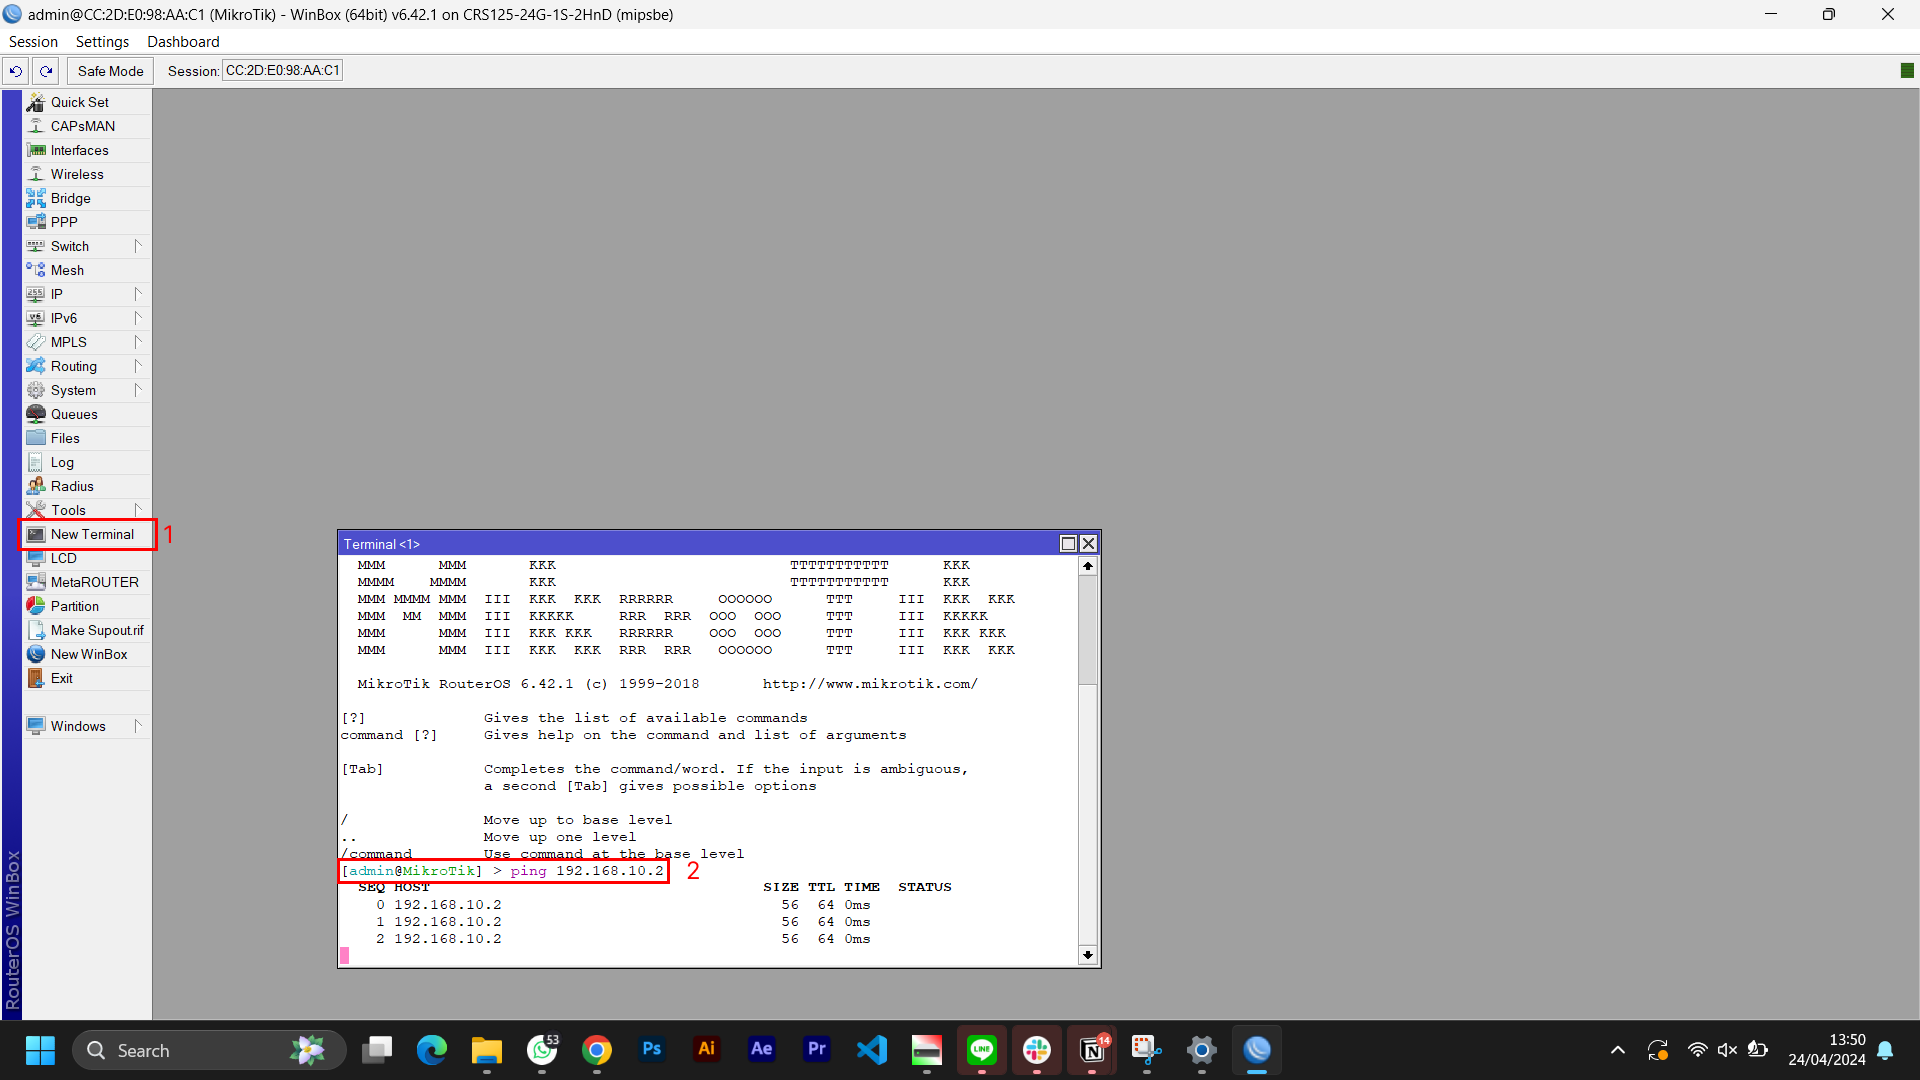
\includegraphics[width=0.9\linewidth]{P2/img/per1/pc2/Step 4.png}
			\caption{Step 2}
			\label{fig:Ping Step 2(Per.1 PC2)}
		\end{figure}
	\end{enumerate}
\end{center}

%======================PERCOBAAN 2==========================%
\subsection{Routing Dinamis}
Pada routing dinamis, terdapat setidaknya 3 jenis, yaitu
\begin{enumerate}
	\item Routing Information Protocol (RIP) RIP adalah salah satu protokol routing dinamis yang menggunakan metrik hop count (jumlah hop) untuk menentukan jalur terbaik. Metrik hop count mengukur jarak antara router pengirim dengan tujuan dalam jumlah hop (melalui berapa banyak router).
	\item Open Shortest Path First (OSPF) OSPF adalah protokol routing dinamis yang menggunakan algoritma Dijkstra untuk menentukan jalur terpendek. OSPF mengumpulkan informasi topologi dari semua router dalam jaringan dan menghitung jalur terbaik berdasarkan bobot (cost) setiap link.
	\item Border Gateway Protocol (BGP) BGP adalah protokol routing eksternal yang digunakan di Internet. BGP memungkinkan router di AS (Autonomous System) yang berbeda untuk berkomunikasi dan menukar informasi routing.
\end{enumerate}

\begin{center}
	\textbf{Konfigurasi Router 1}
	\begin{enumerate}
		\item Buka WinBox dan lakukan koneksi ke Router 1
		\item Berikan IP address pada interface ether2 dan ether 4 yang dapat dibuat pada tab IP > Addresses. Berikan IP address sesuai dengan cara pengaturan IP address yang benar Berikan IP address yang berbeda dengan contoh di modul.
		\begin{figure}[H]
			\centering
			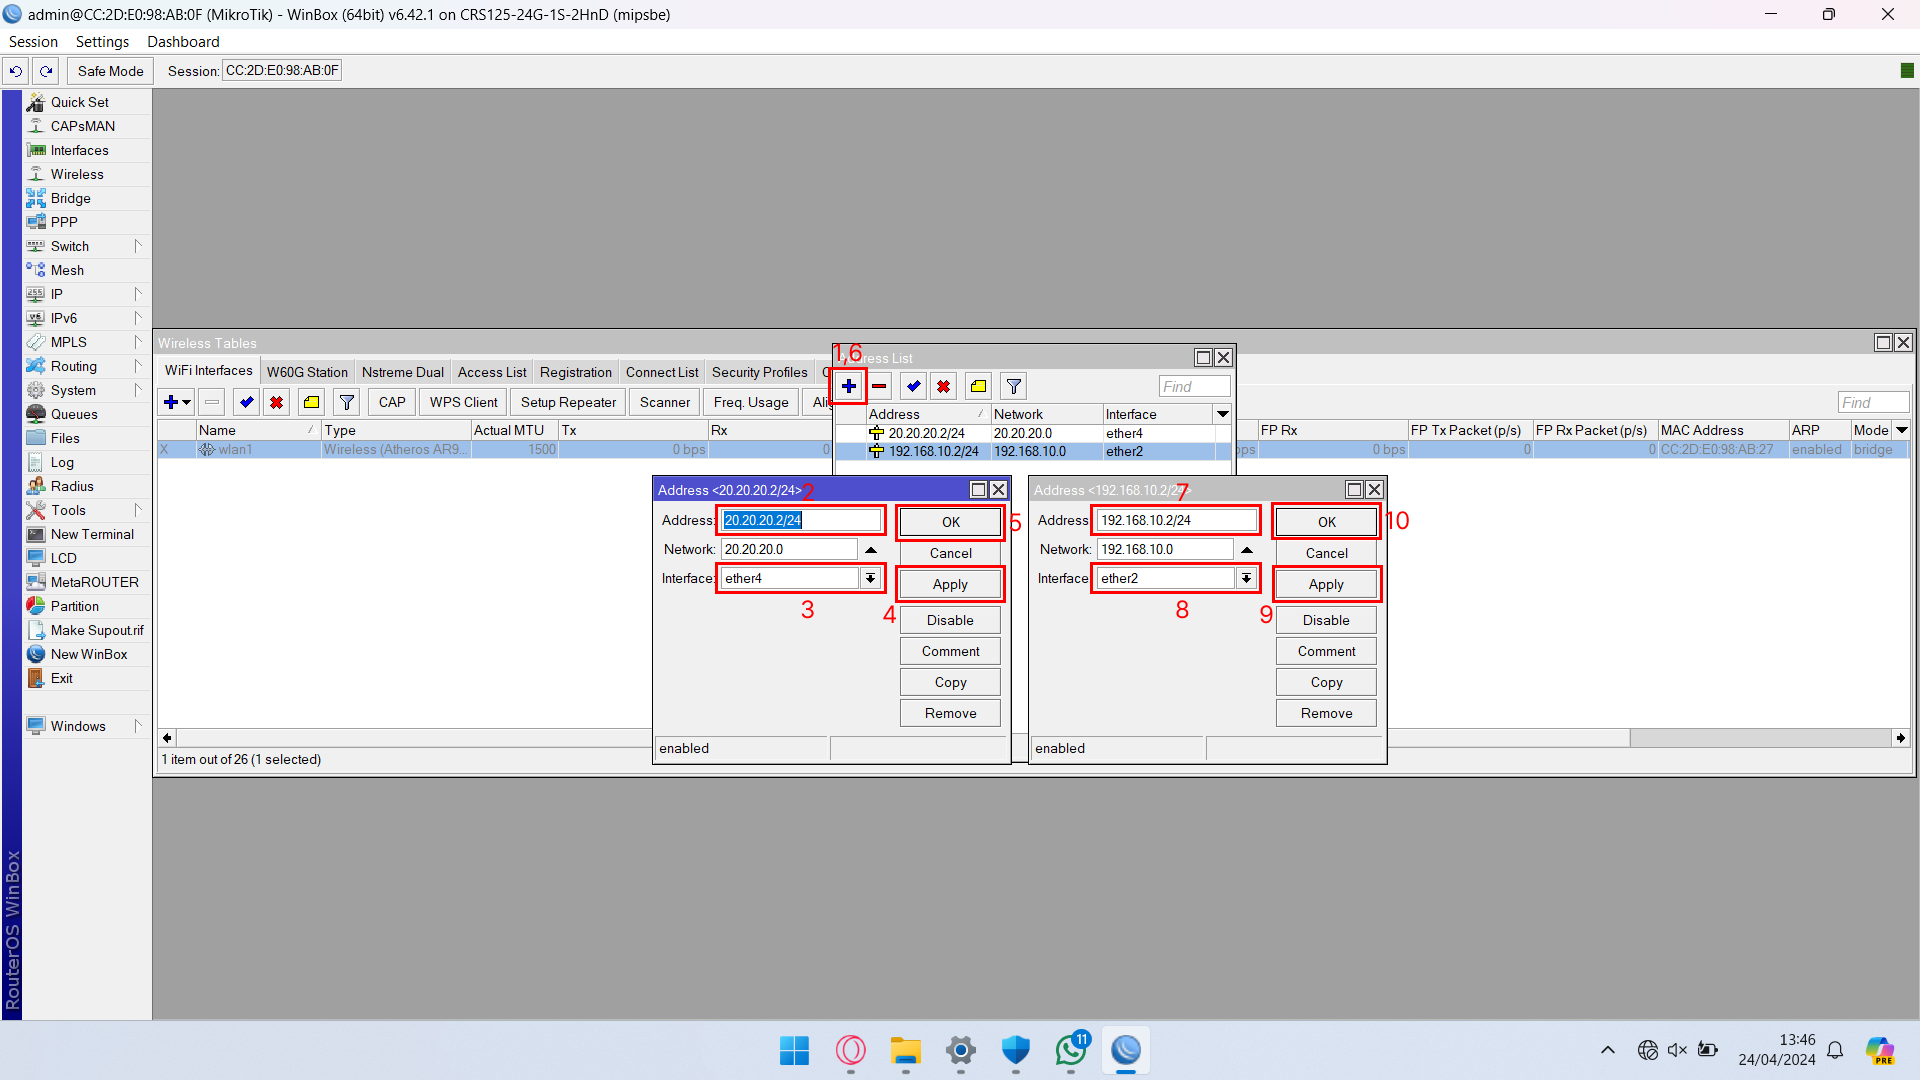
\includegraphics[width=0.9\linewidth]{P2/img/per1/pc1/Step 2.png}
			\caption{Step 2}
			\label{fig:Step 2(Per.2 PC1)}
		\end{figure}
		\item Pada PC 1, lakukan routing dinamis. Buka tab Routing > RIP. 
		\begin{figure}[H]
			\centering
			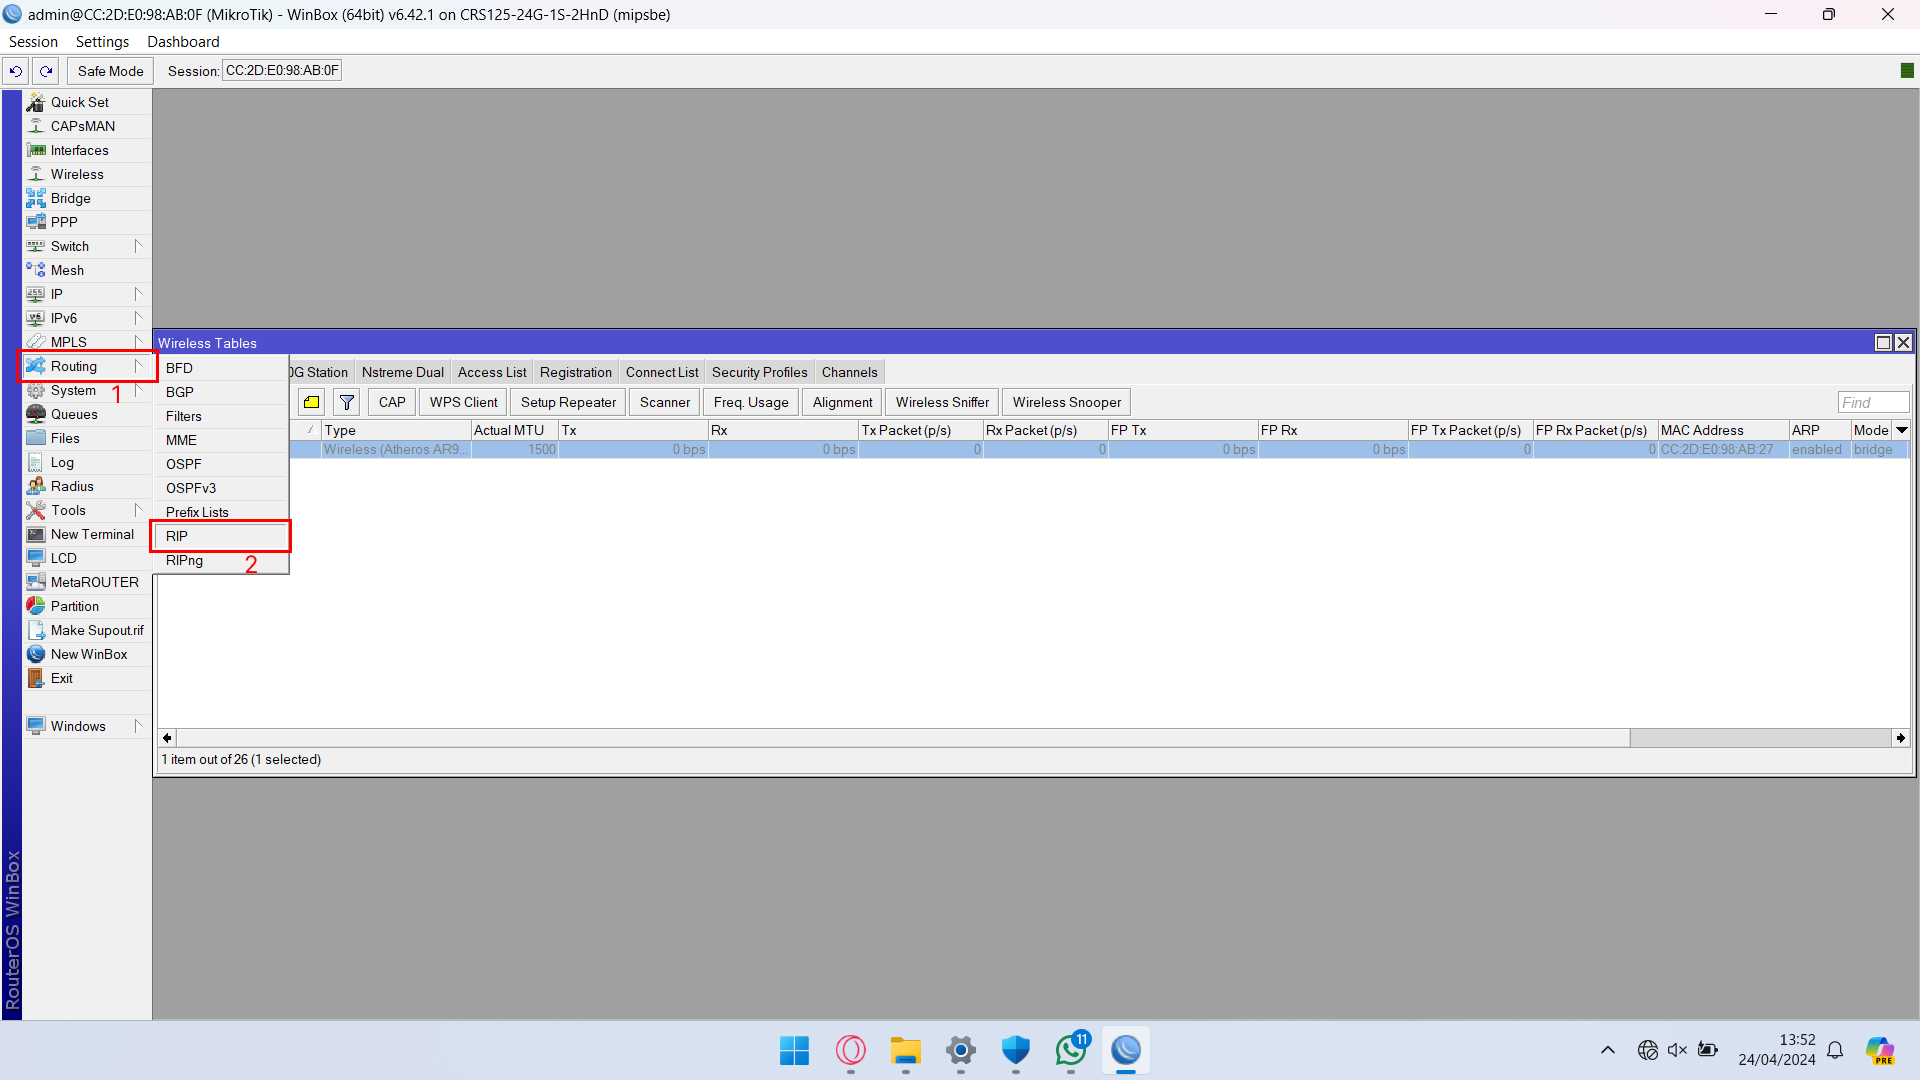
\includegraphics[width=0.9\linewidth]{P2/img/per2/pc1/Step 3.1.png}
			\caption{Step 3.1}
			\label{fig:Step 3.1(Per.2 PC1)}
		\end{figure}
		Pada interface tambahkan interface baru kemudian ubah interface menjadi ether 4 dengan Receive dan Send pada v1.
		\begin{figure}[H]
			\centering
			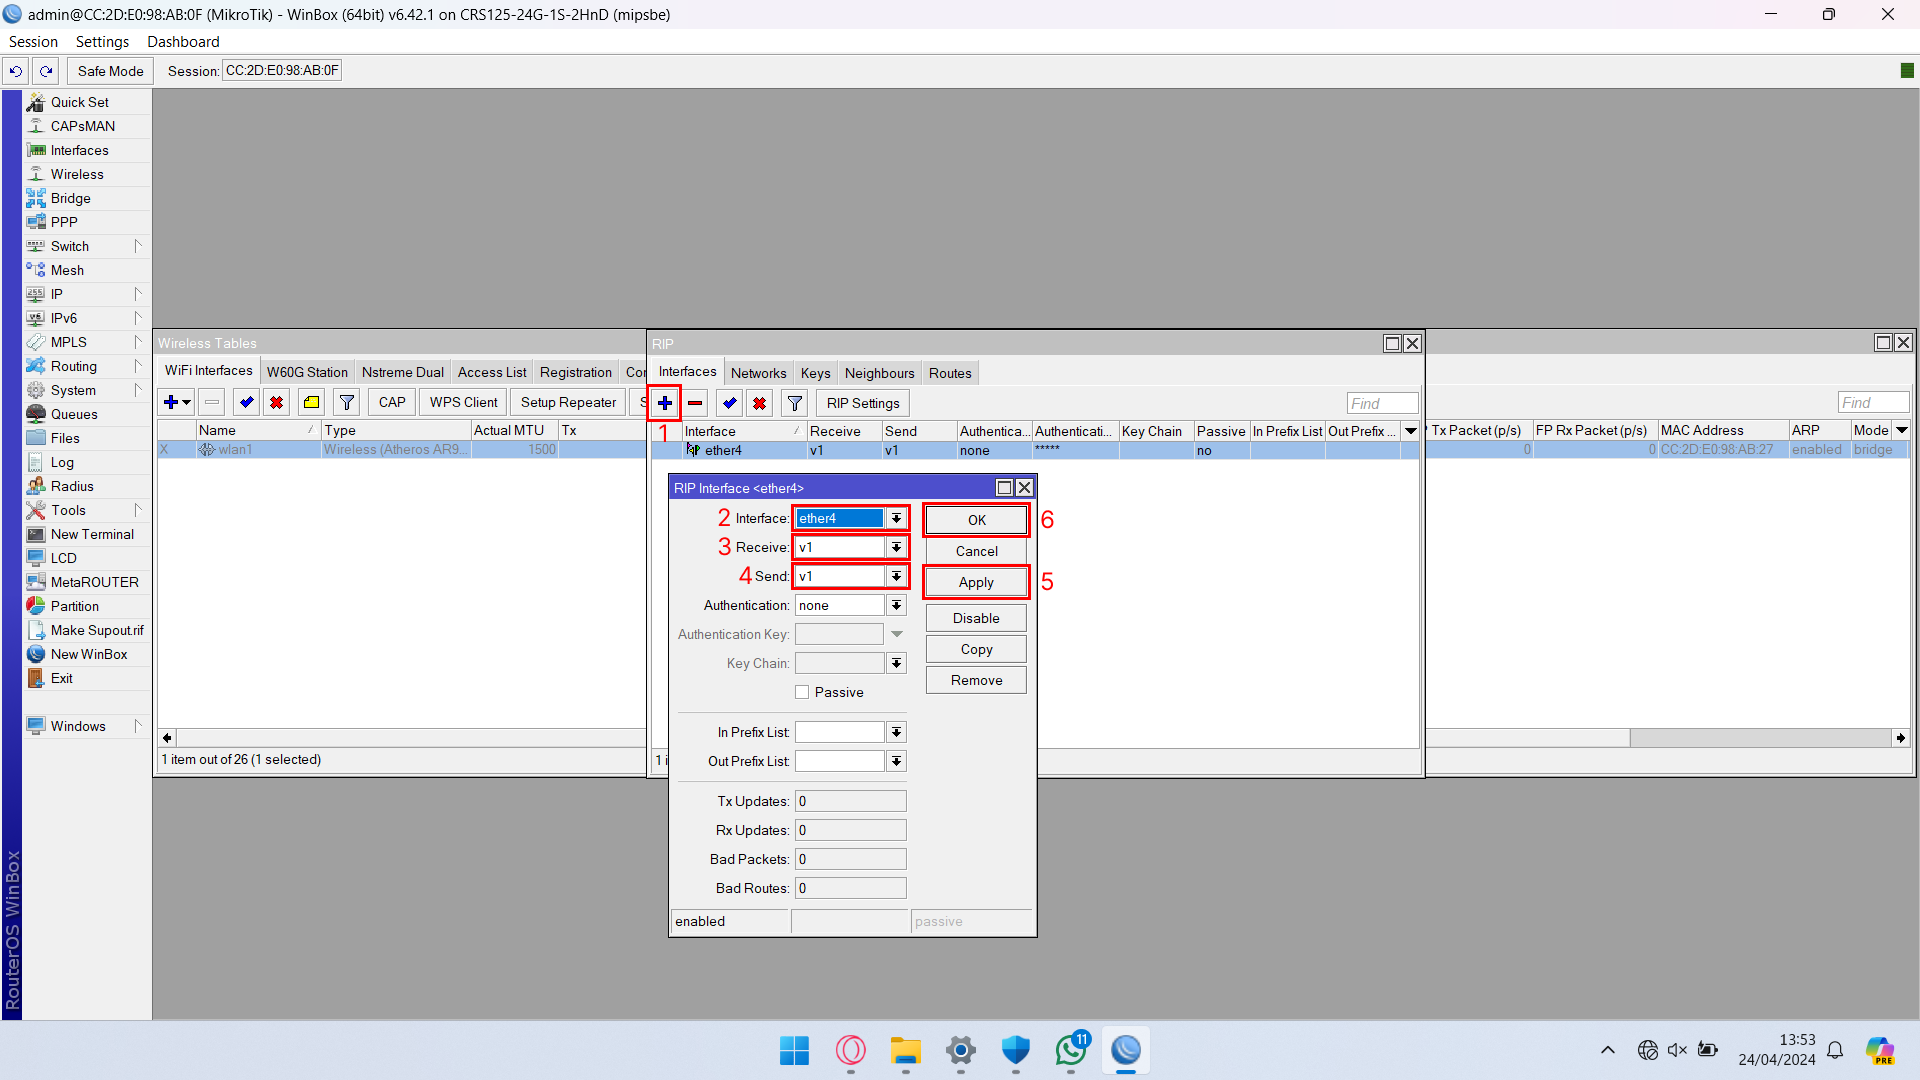
\includegraphics[width=0.9\linewidth]{P2/img/per2/pc1/Step 3.2.png}
			\caption{Step 3.2}
			\label{fig:Step 3.2(Per.2 PC1)}
		\end{figure}
		\item Pada tab Network, tambahkan 2 network baru, yaitu network yang antara PC1 dengan Router 1 dan network antara Router 1 dan Router 2.
		\begin{figure}[H]
			\centering
			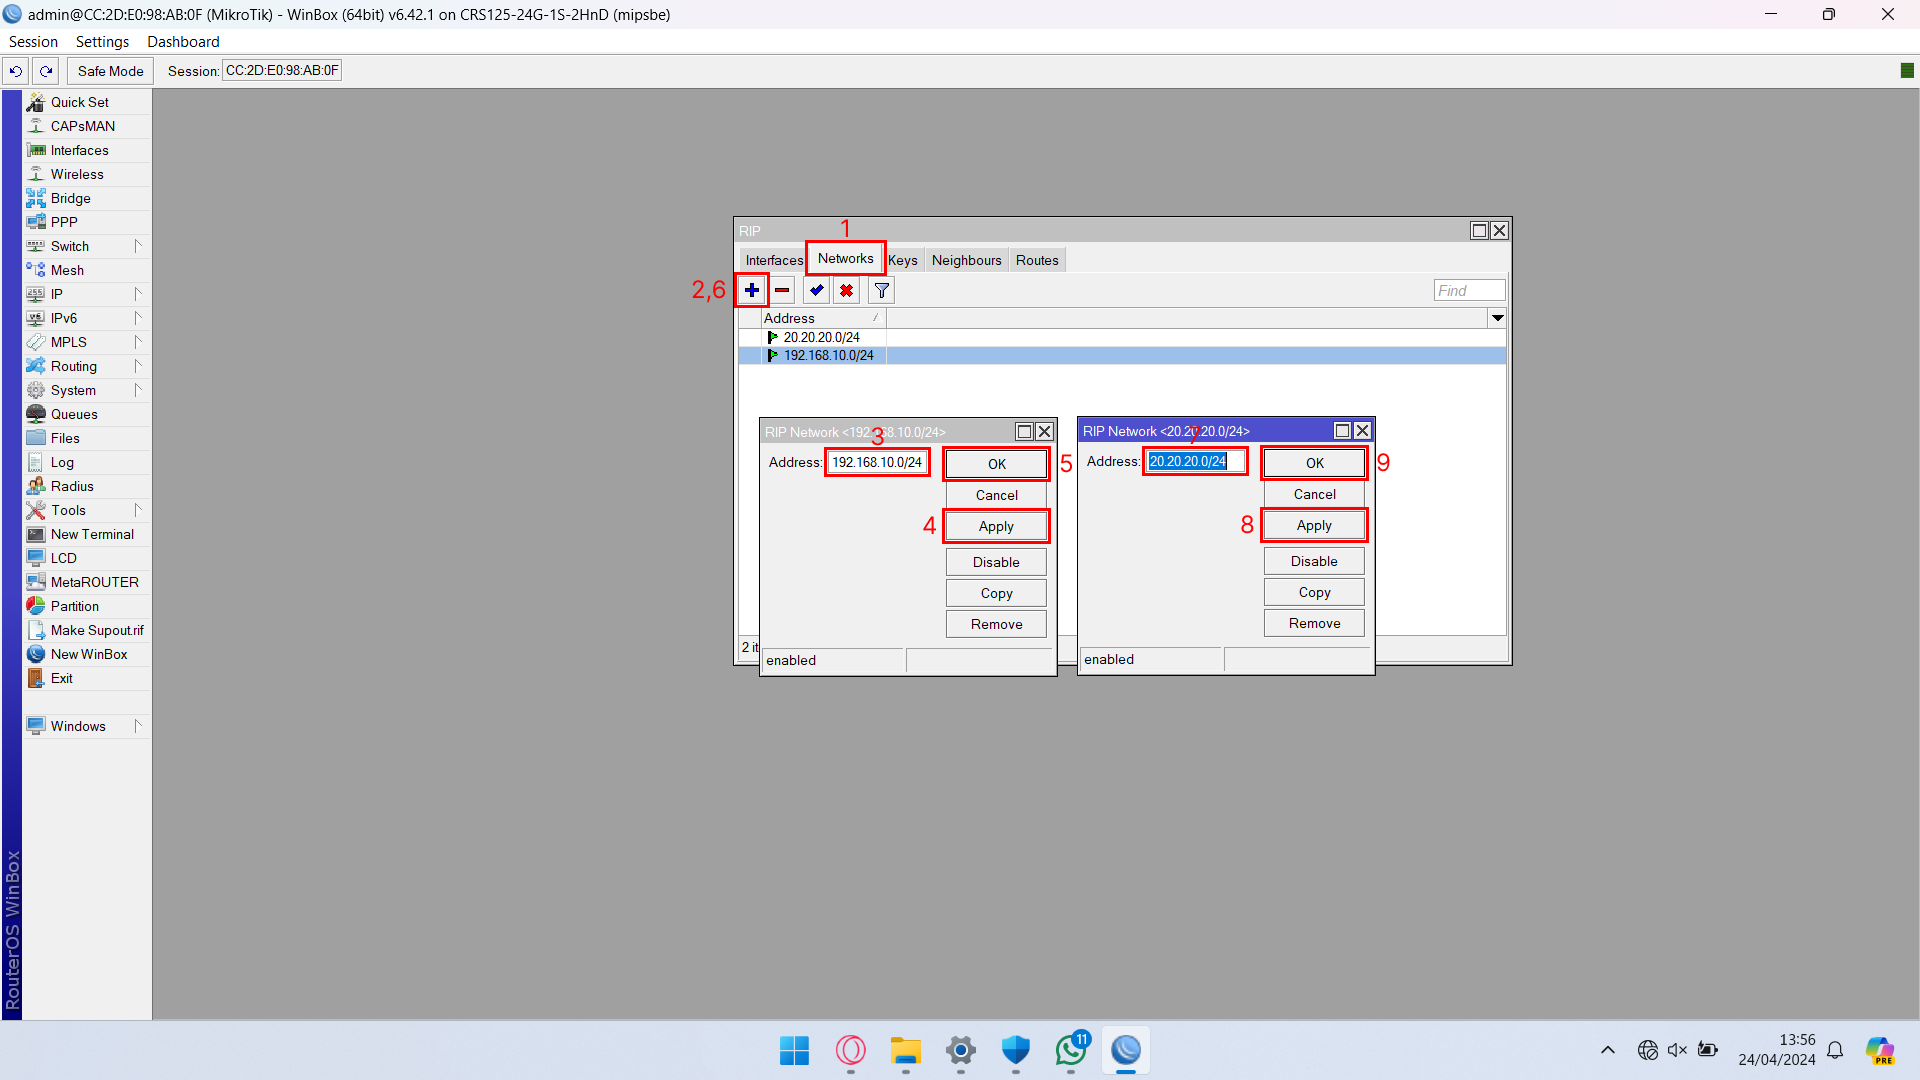
\includegraphics[width=0.9\linewidth]{P2/img/per2/pc1/Step 4.png}
			\caption{Step 4}
			\label{fig:Step 4(Per.2 PC1)}
		\end{figure}
		\item Pada tab Neighbours, tambahkan alamat router yang dituju.
		\begin{figure}[H]
			\centering
			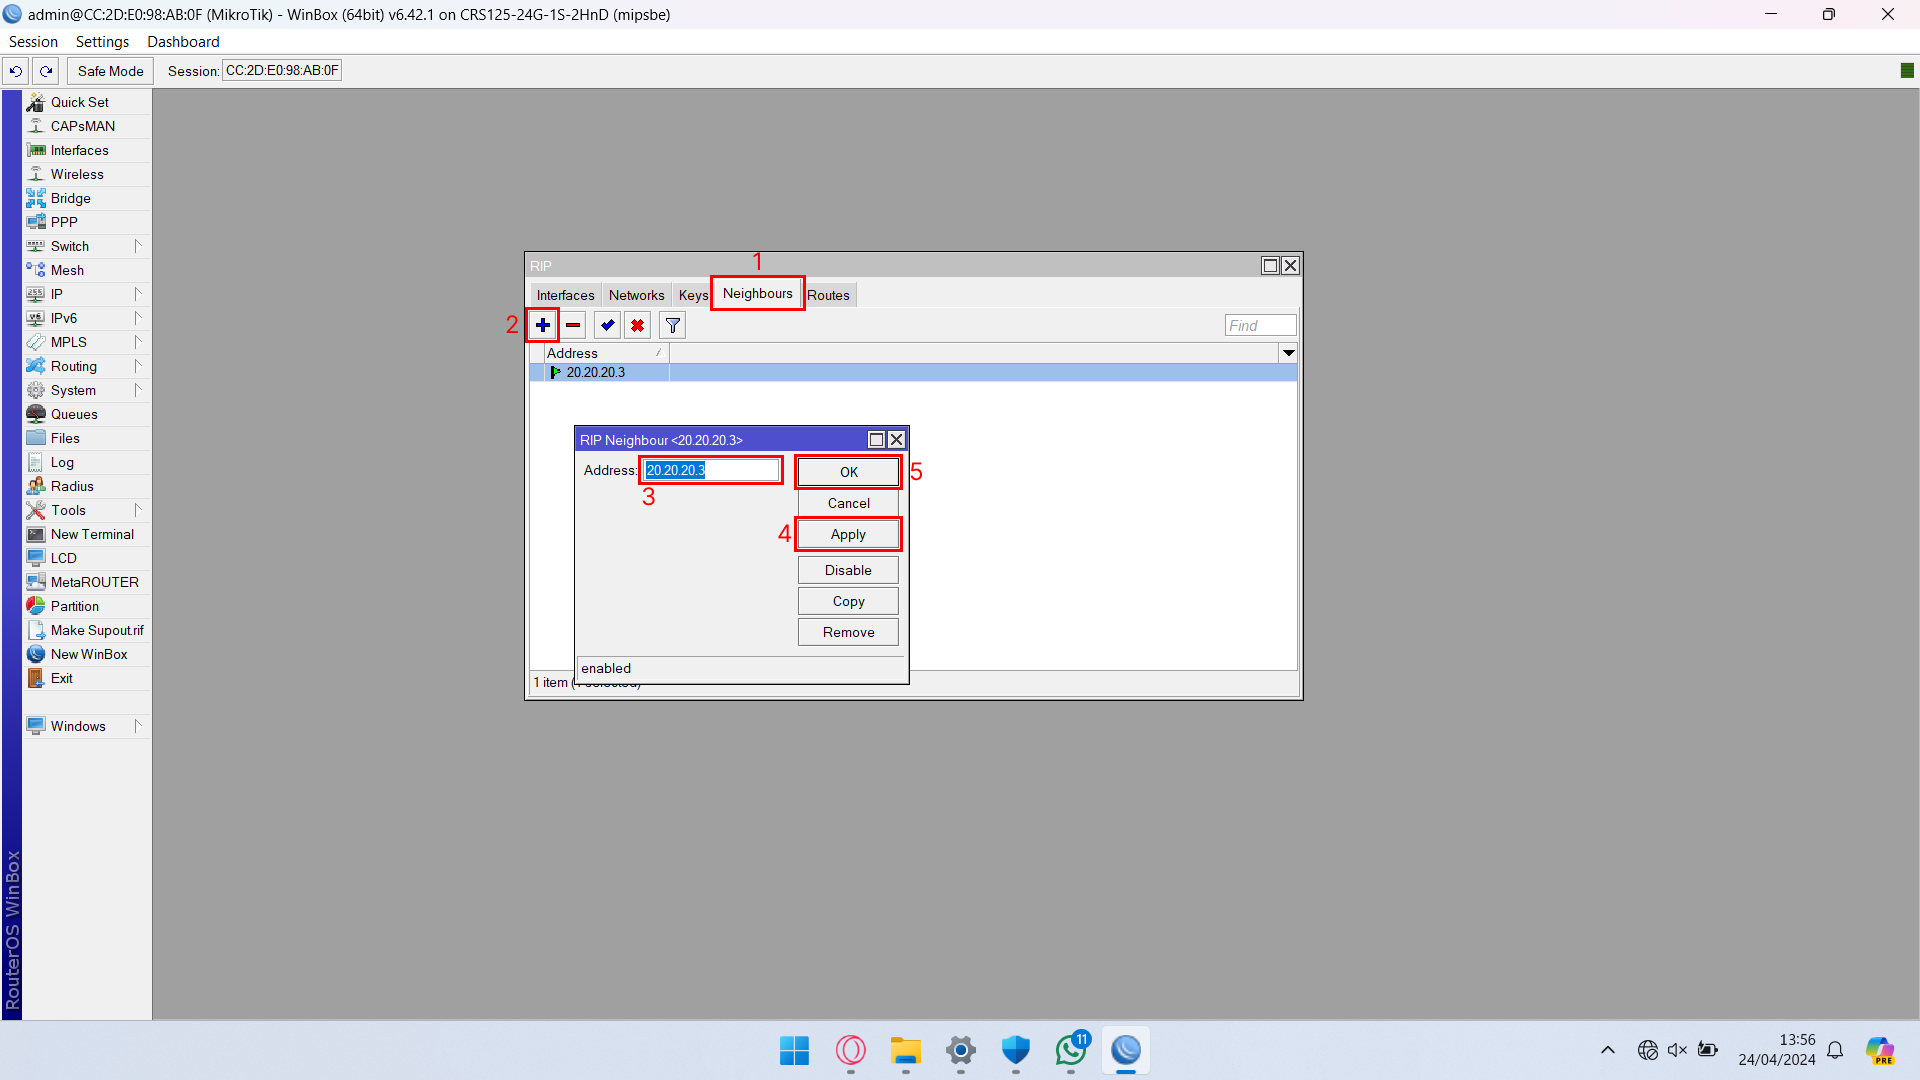
\includegraphics[width=0.9\linewidth]{P2/img/per2/pc1/Step 5.png}
			\caption{Step 5}
			\label{fig:Step 5(Per.2 PC1)}
		\end{figure}
	\end{enumerate}

	\textbf{Konfigurasi Router2}
	\begin{enumerate}
		\item Buka WinBox dan lakukan koneksi ke Router 2
		\item Berikan IP address pada interface ether2 dan ether 4 yang dapat dibuat pada tab IP > Addresses. Berikan IP address sesuai dengan cara pengaturan IP address yang benar. Berikan IP address yang berbeda dengan contoh di modul.
		\begin{figure}[H]
			\centering
			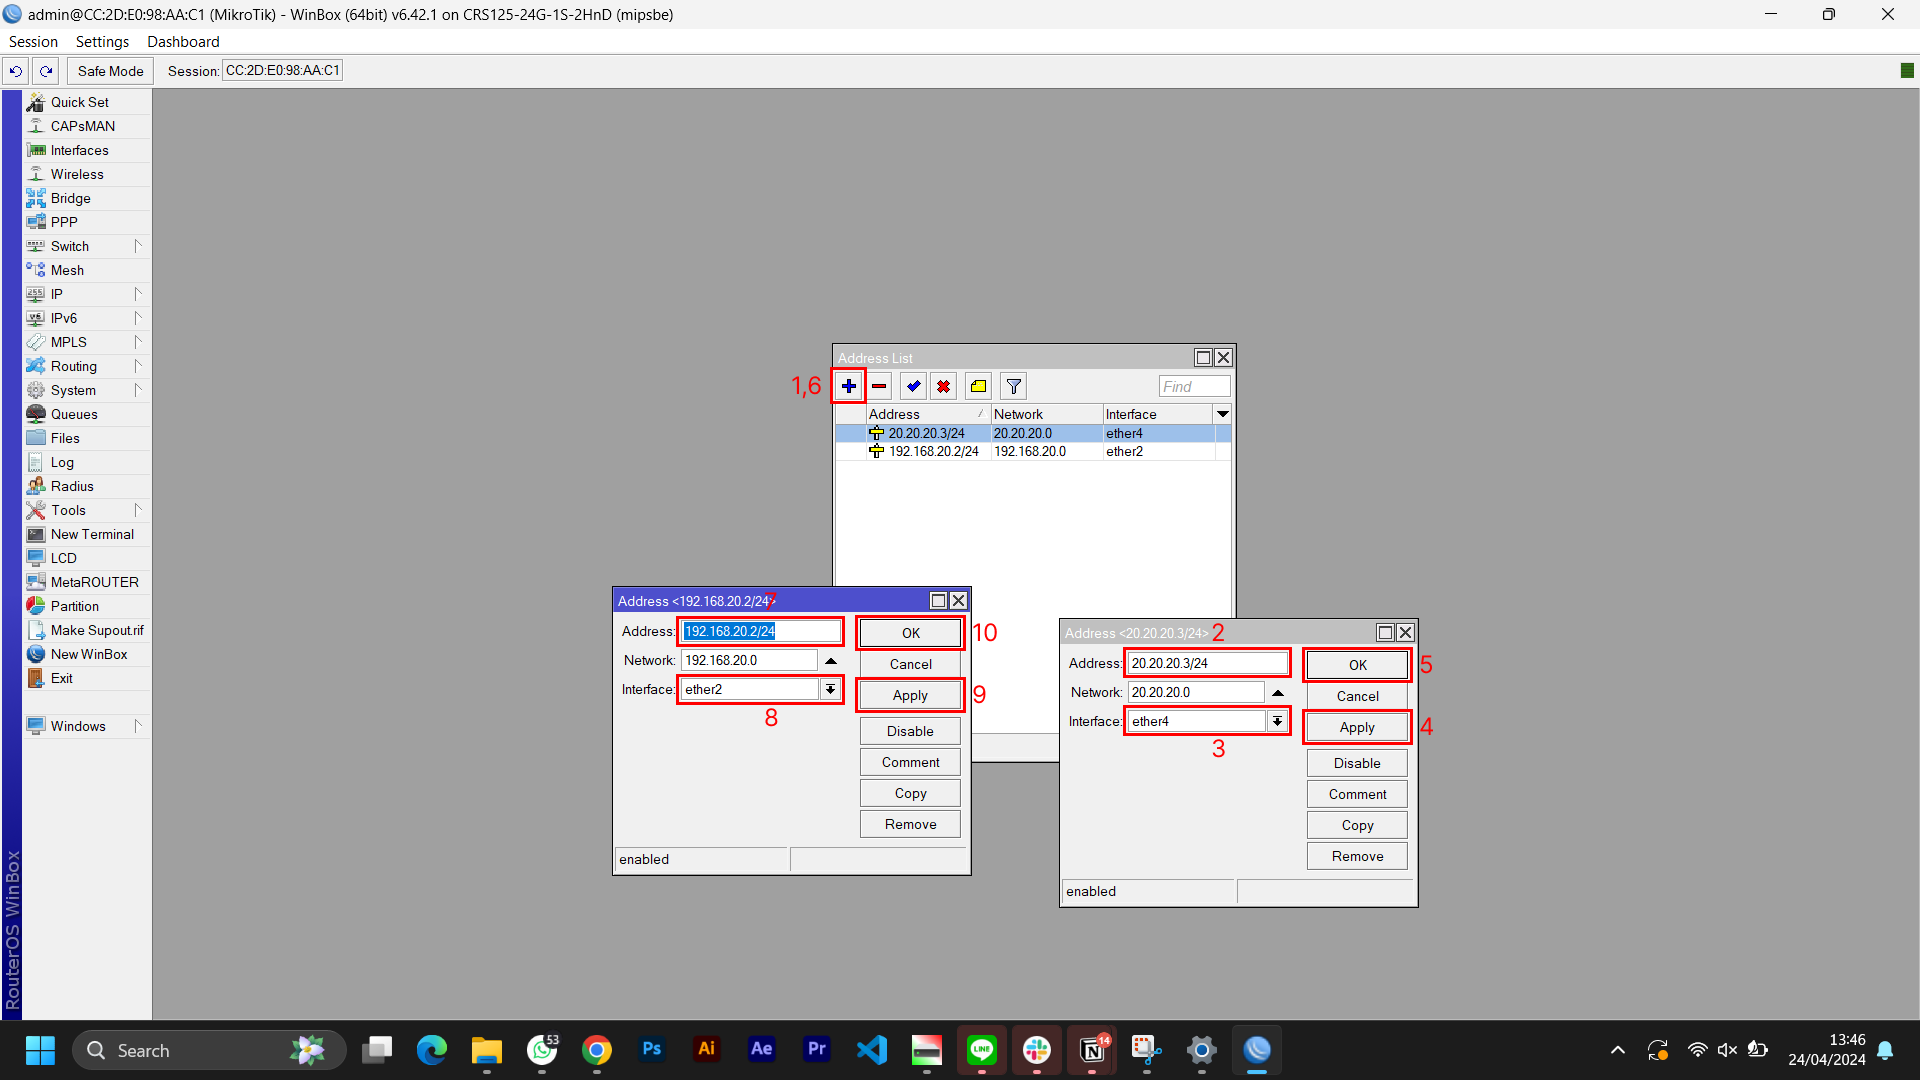
\includegraphics[width=0.9\linewidth]{P2/img/per1/pc2/Step 2.png}
			\caption{Step 2}
			\label{fig:Step 2(Per.2 PC2)}
		\end{figure}
		\item Pada interface tambahkan interface baru kemudian ubah interface menjadi ether 4 dengan Receive dan Send pada v1.
		\begin{figure}[H]
			\centering
			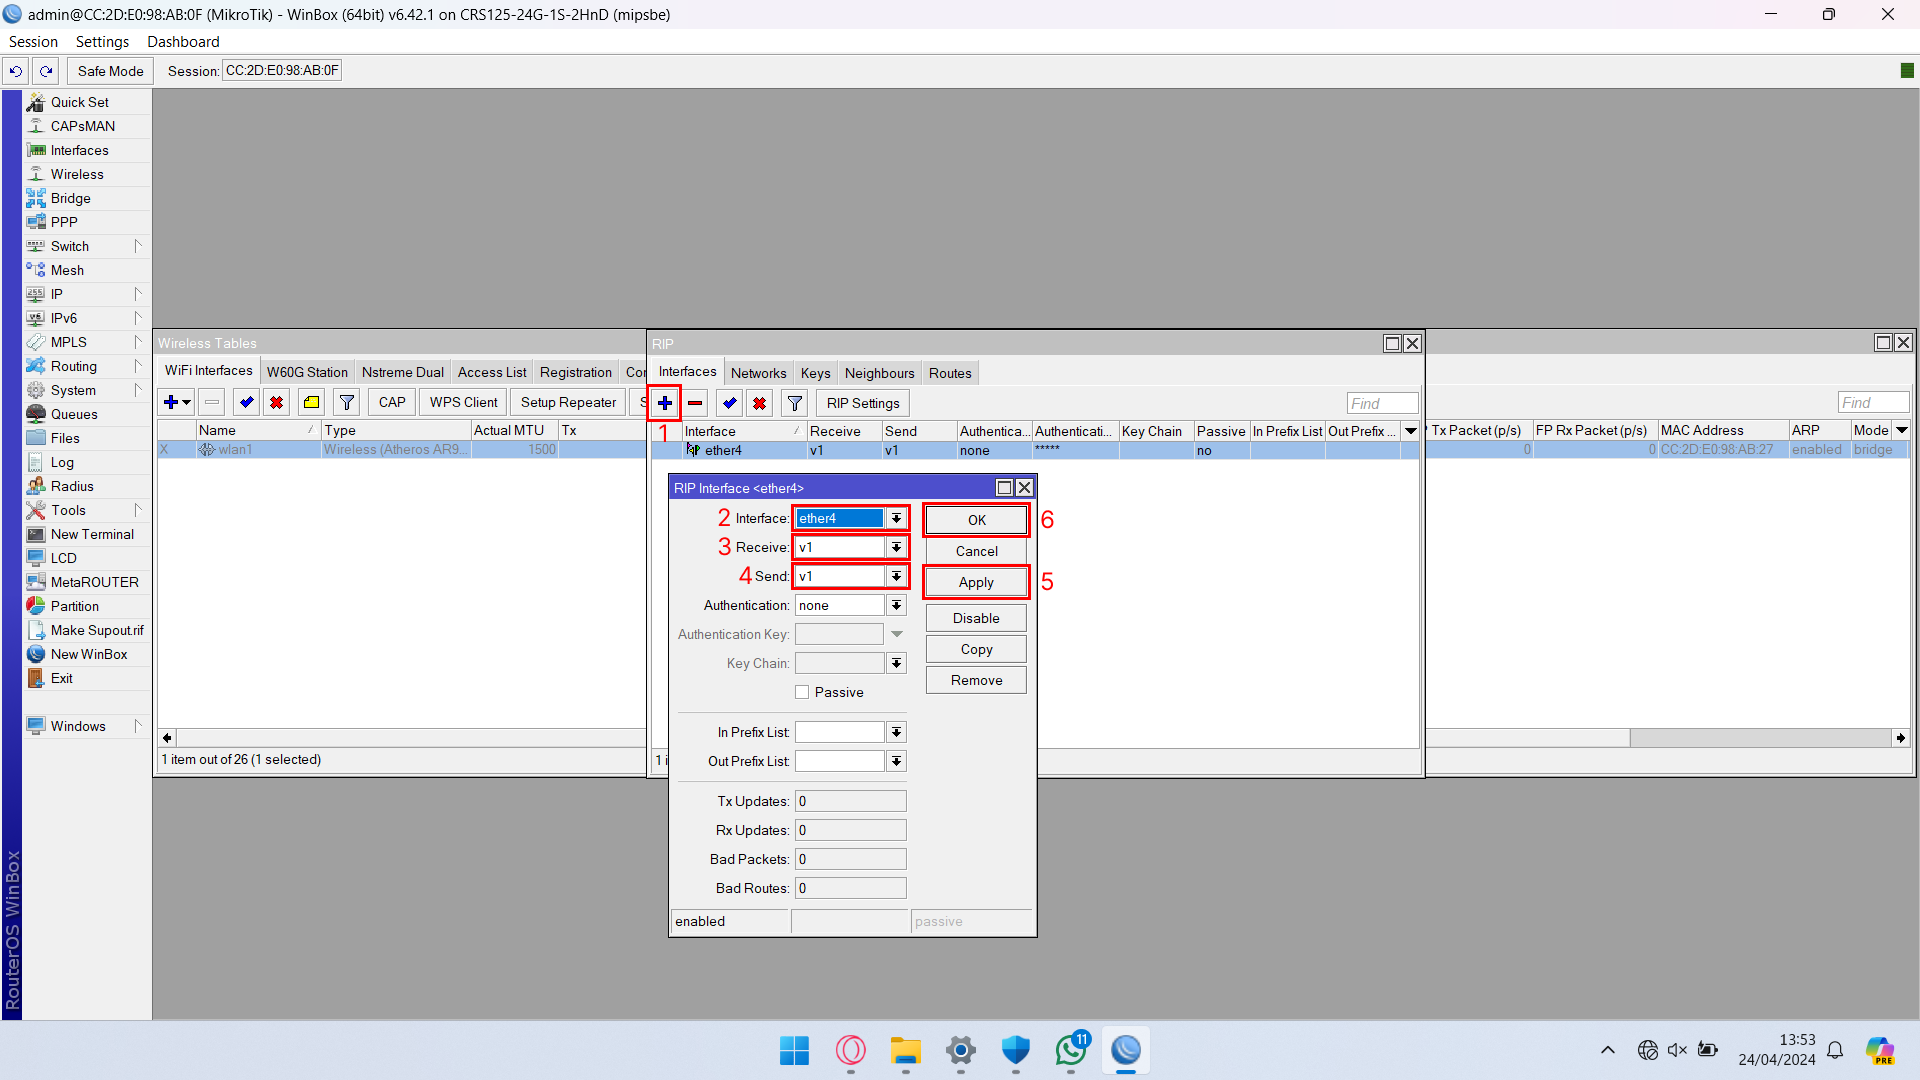
\includegraphics[width=0.9\linewidth]{P2/img/per2/pc1/Step 3.2.png}
			\caption{Step 3.1}
			\label{fig:Step 3.1(Per.2 PC2)}
		\end{figure}
		\item Pada tab Network, tambahkan 2 network baru, yaitu network yang antara PC2 dengan Router 2 dan network antara Router 1 dan Router 2.
		\begin{figure}[H]
			\centering
			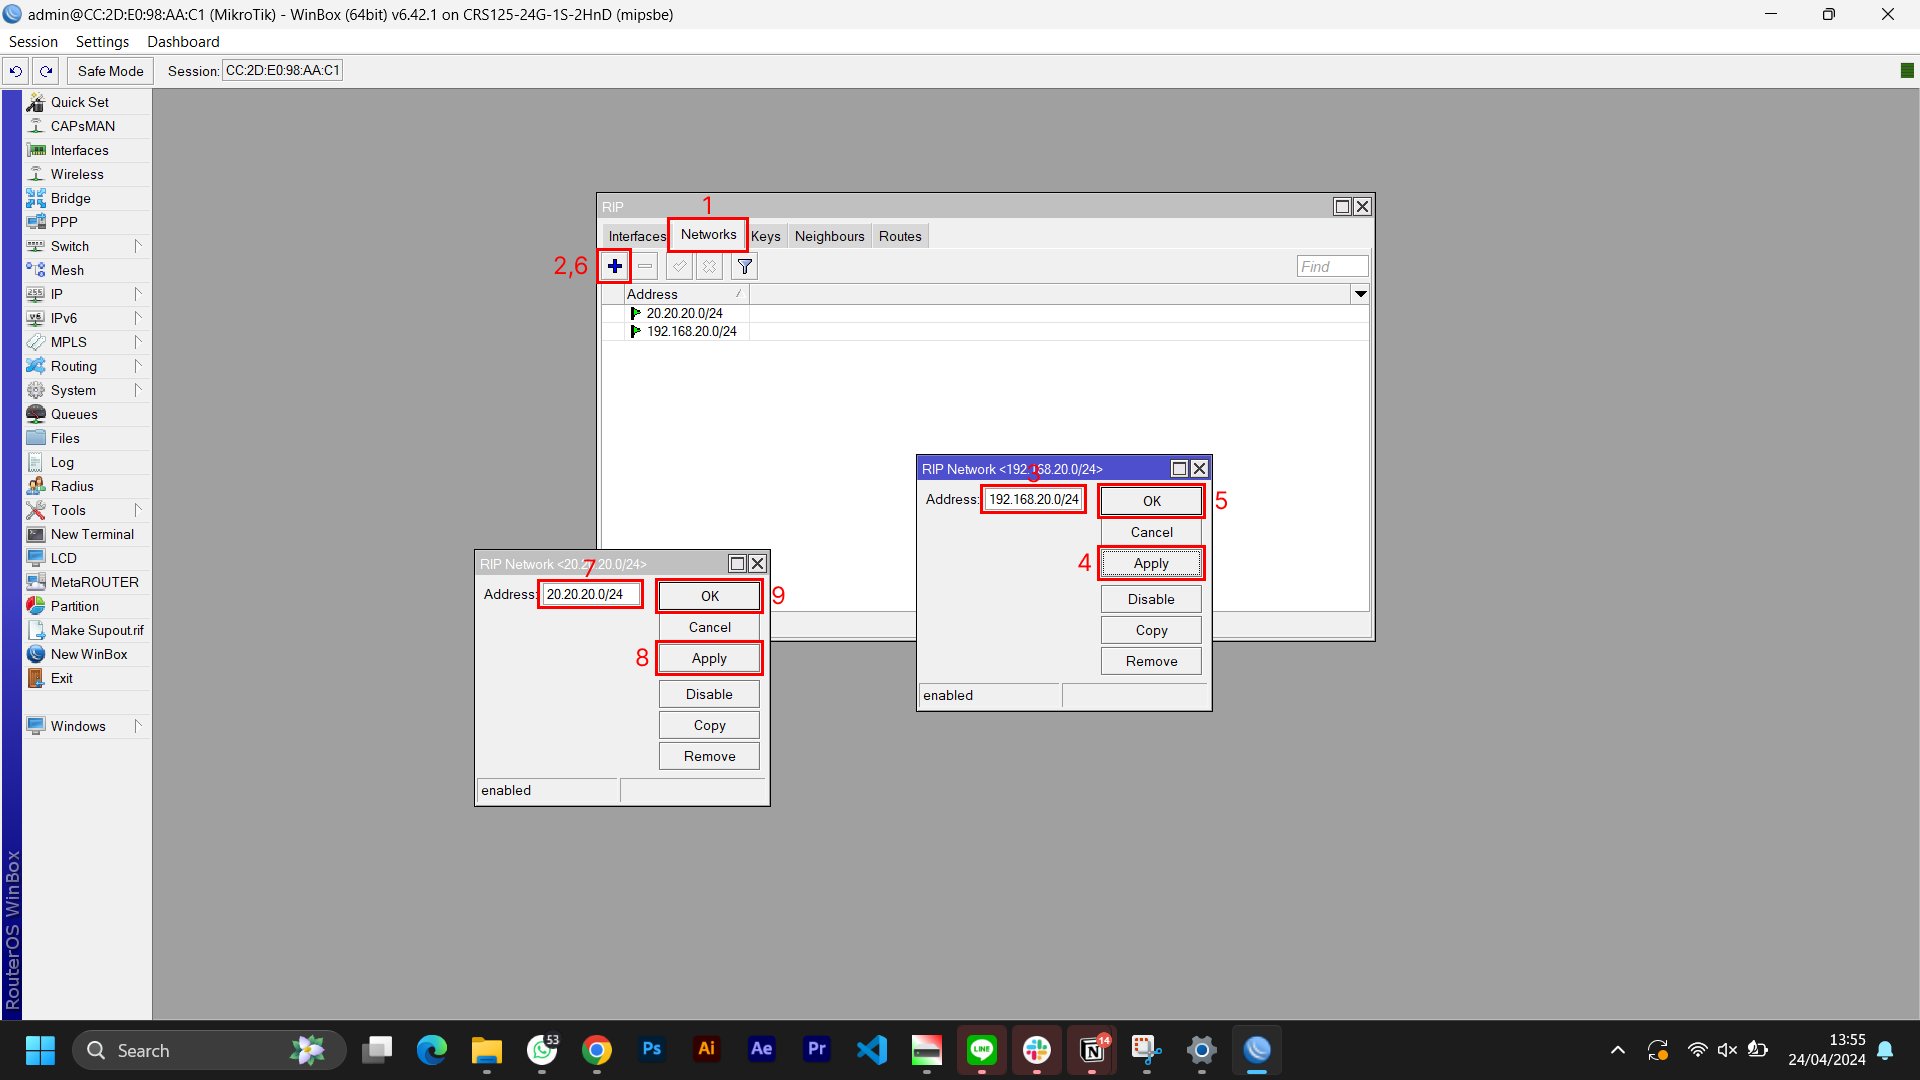
\includegraphics[width=0.9\linewidth]{P2/img/per2/pc2/Step 4.png}
			\caption{Step 3.2}
			\label{fig:Step 3.2(Per.2 PC2)}
		\end{figure}
		\item Pada tab Neighbours, tambahkan alamat router yang dituju.
		\begin{figure}[H]
			\centering
			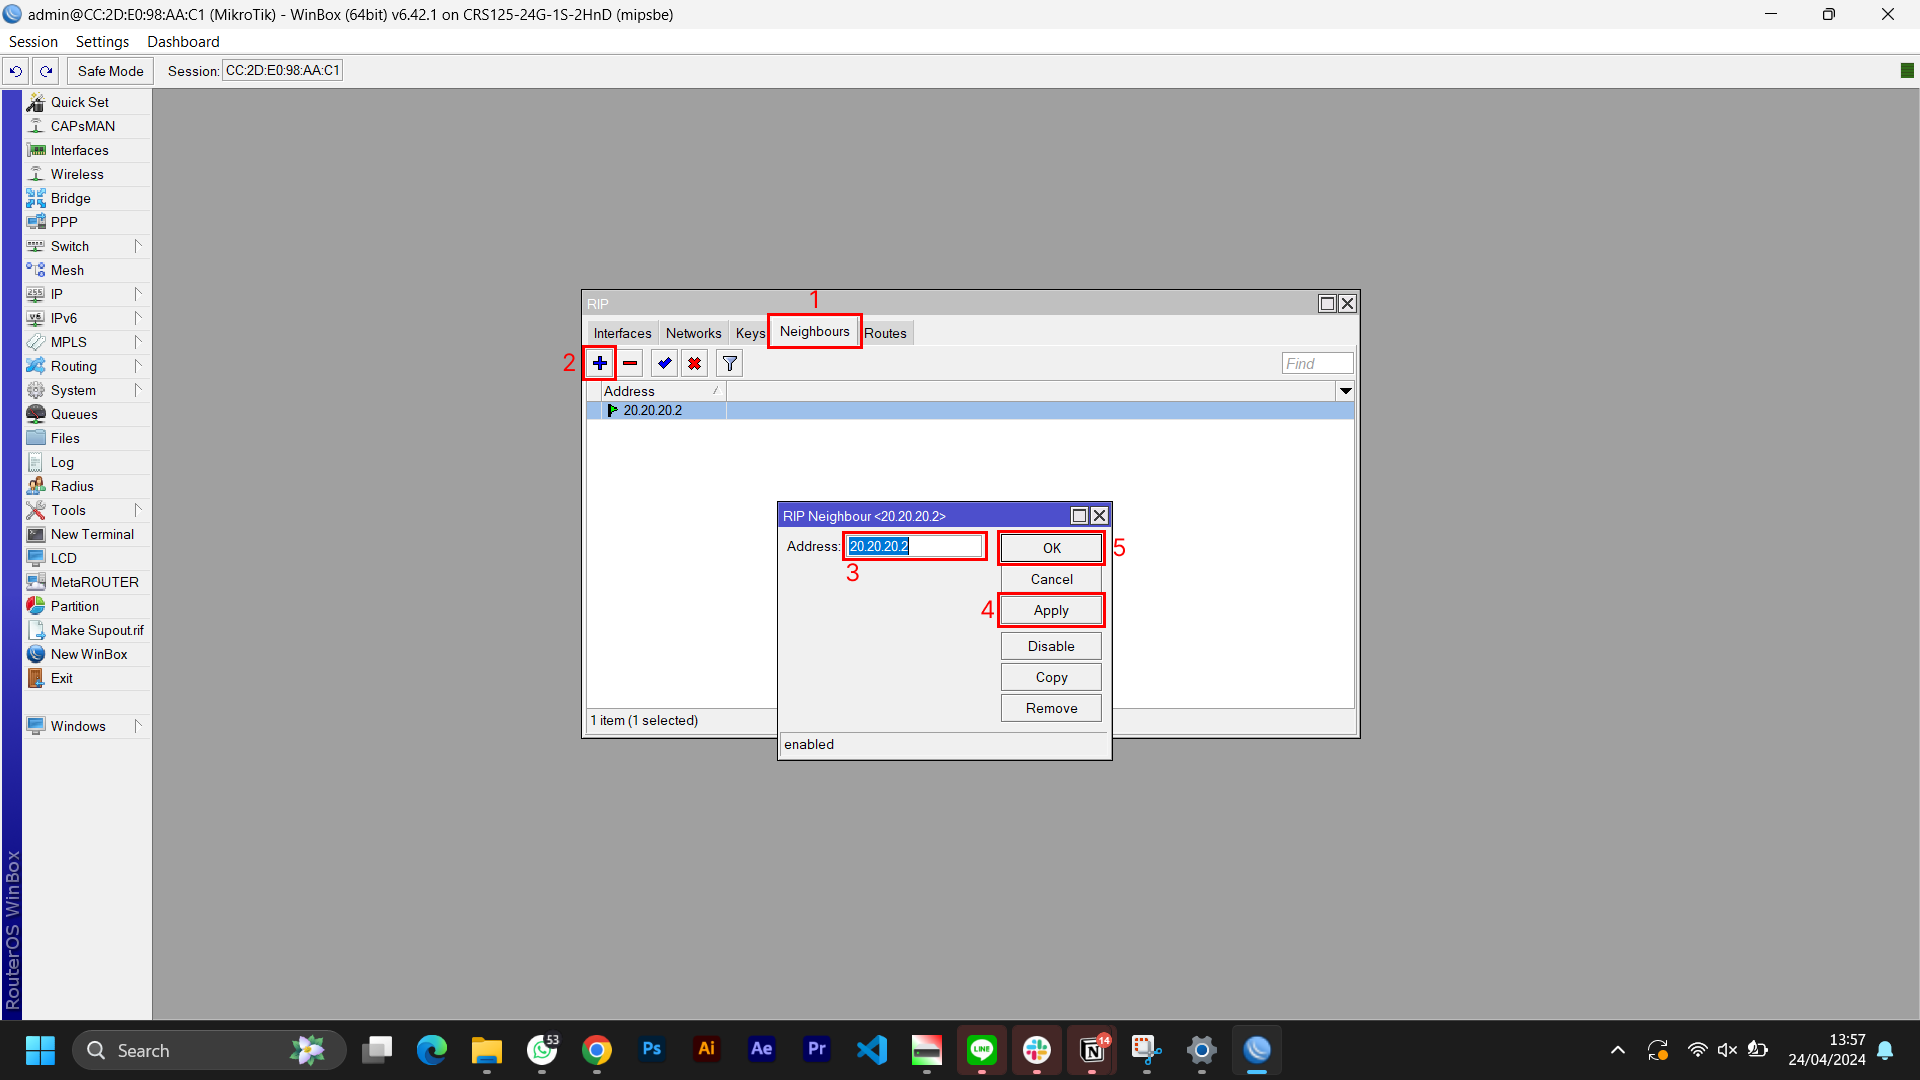
\includegraphics[width=0.9\linewidth]{P2/img/per2/pc2/Step 5.png}
			\caption{Step 4}
			\label{fig:Step 4(Per.2 PC2)}
		\end{figure}
	\end{enumerate}

	\textbf{Pengujian Konfigurasi}
	\begin{enumerate}
		\item Lakukan tes ping dari Router 2 ke Router 1
		\begin{figure}[H]
			\centering
			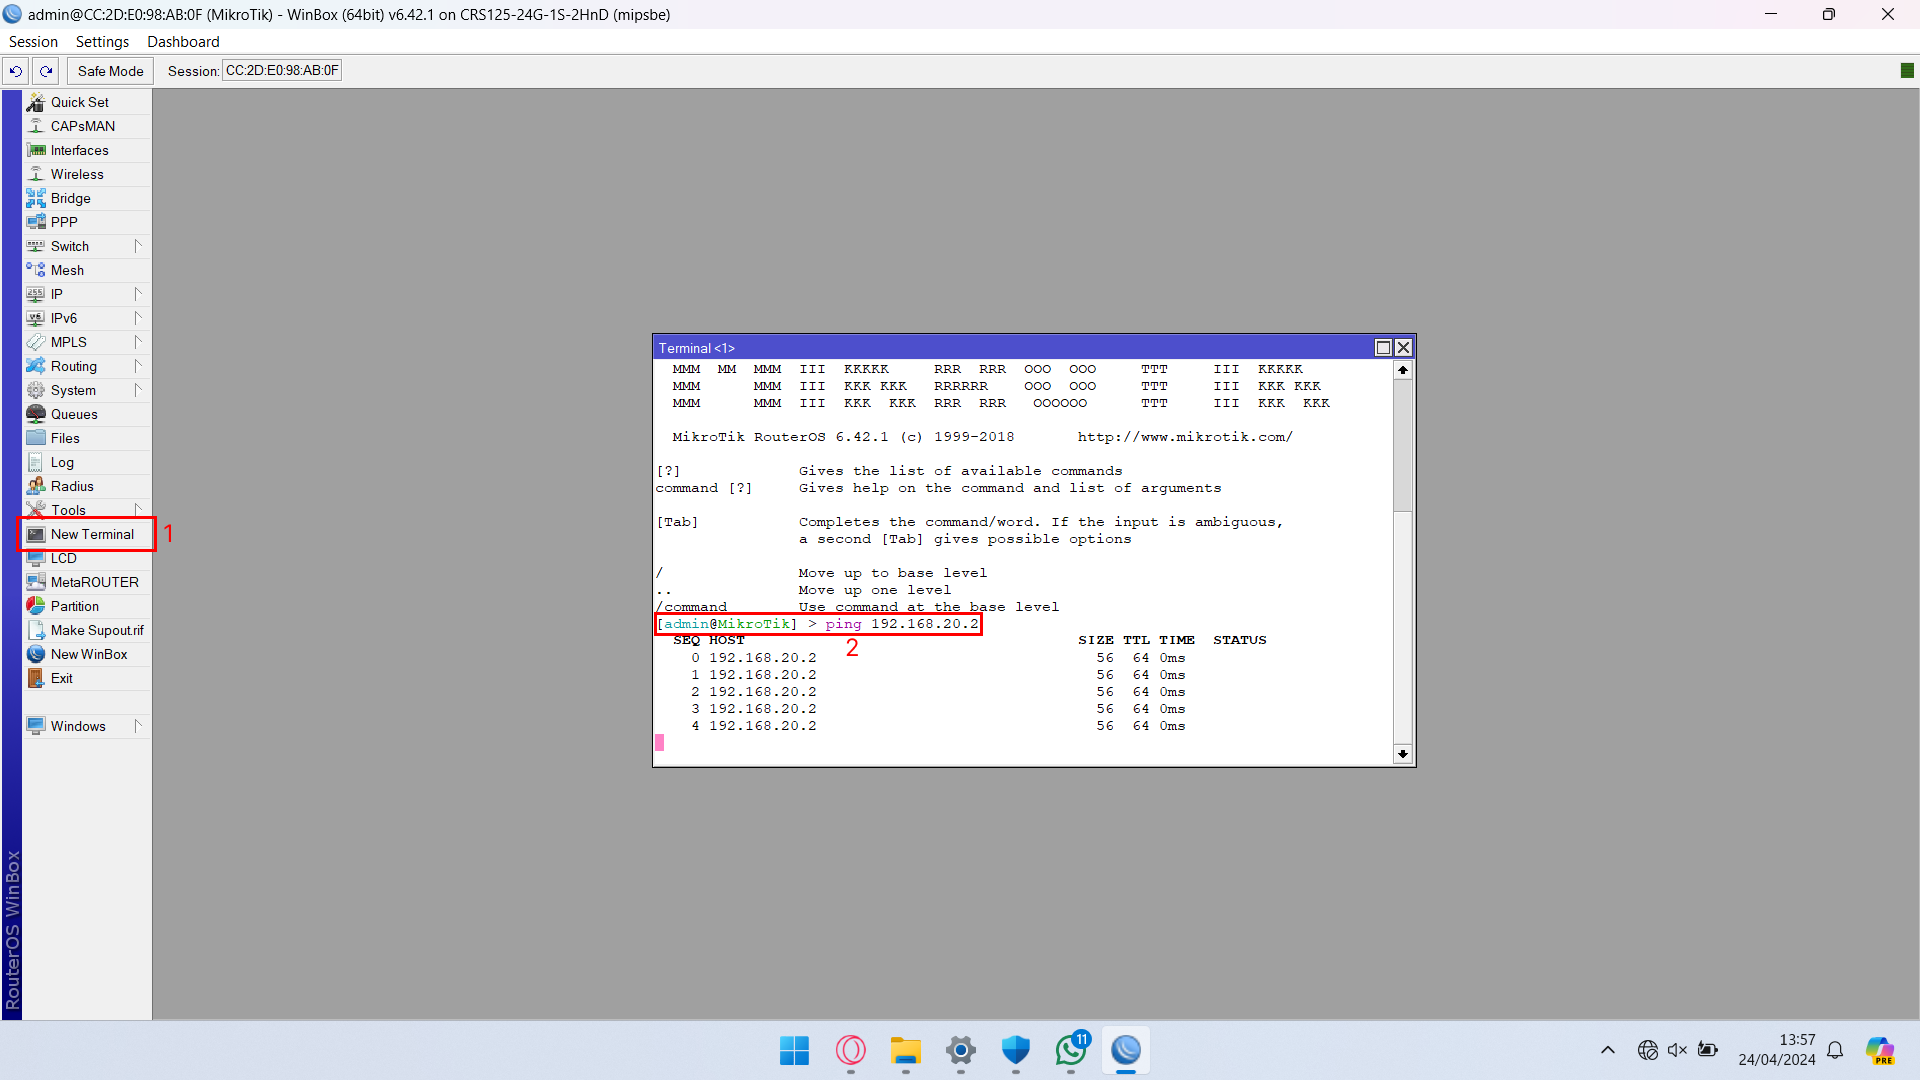
\includegraphics[width=0.9\linewidth]{P2/img/per2/pc1/Step 6.png}
			\caption{Step 1}
			\label{fig:Ping Step 1(Per.2 PC1)}
		\end{figure}
		\item Lakukan tes ping dari Router 1 ke Router 2
		\begin{figure}[H]
			\centering
			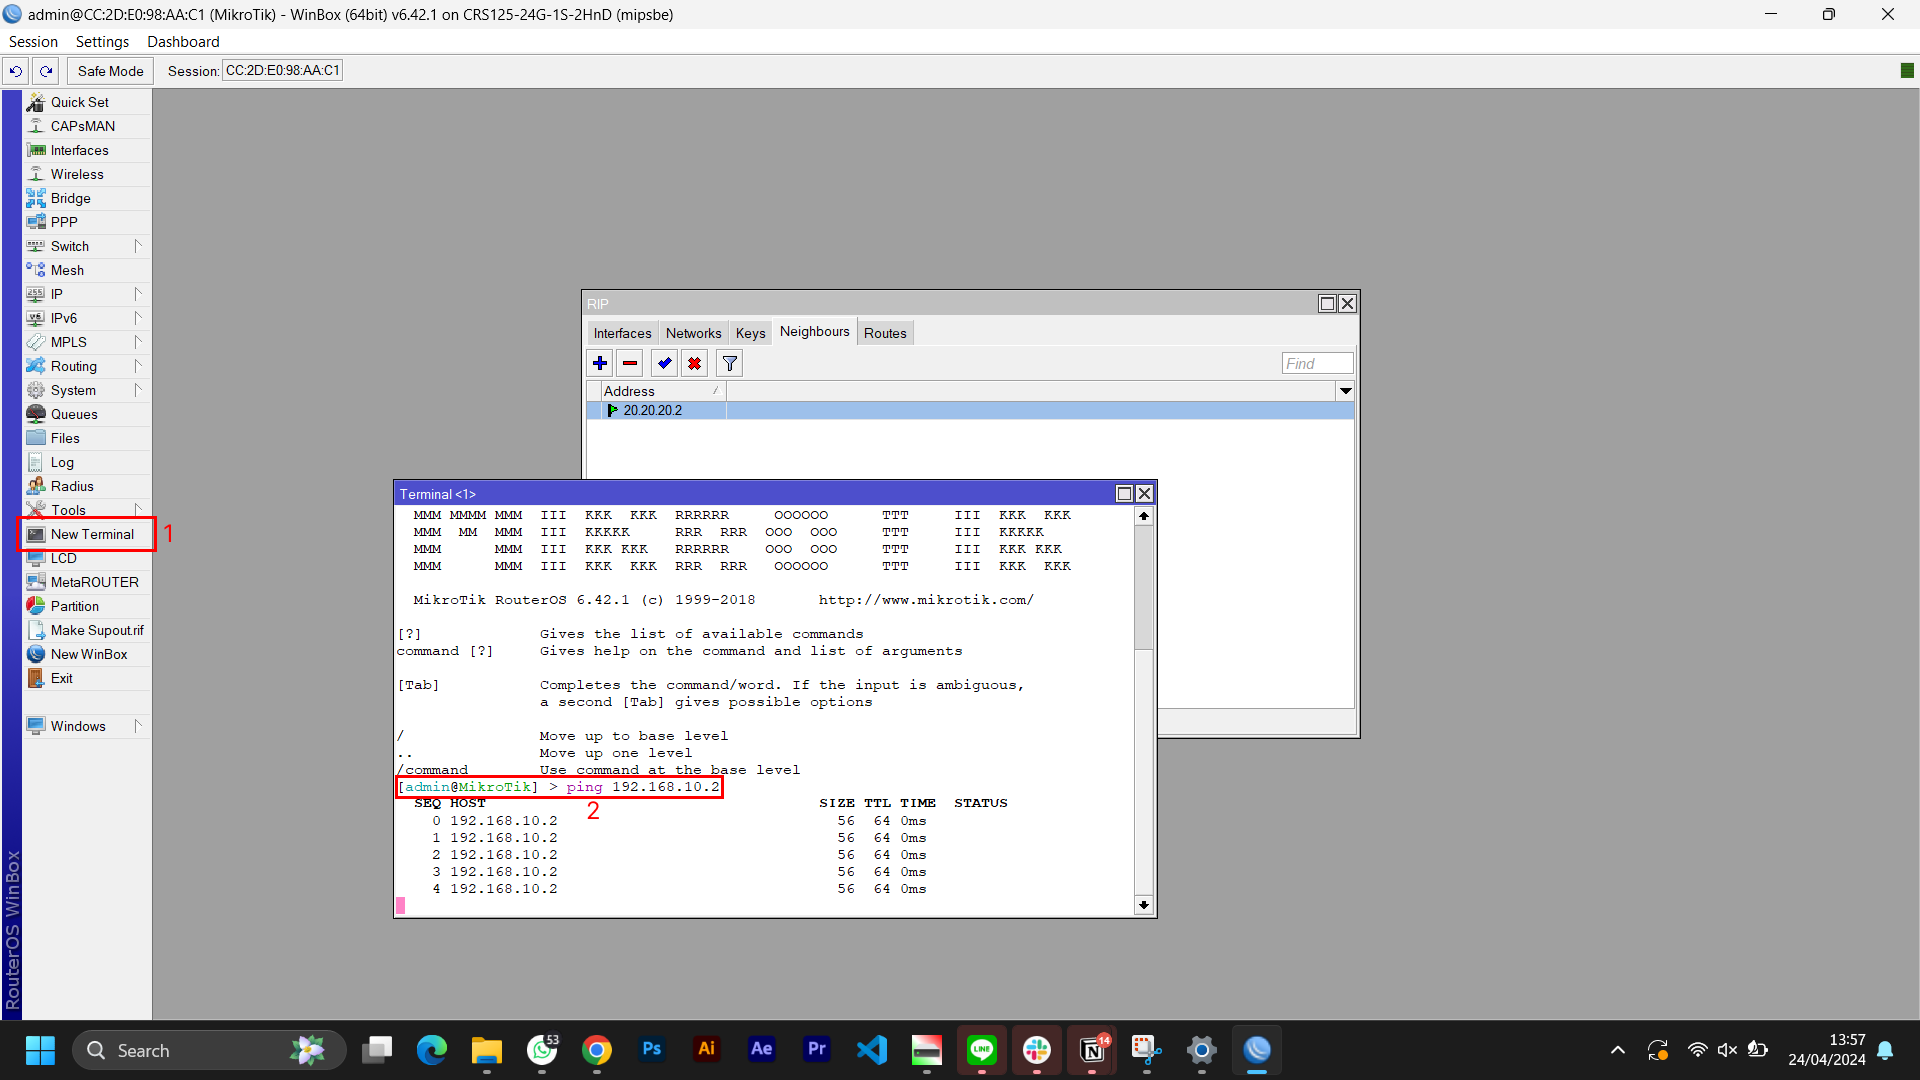
\includegraphics[width=0.9\linewidth]{P2/img/per2/pc2/Step 6.png}
			\caption{Step 2}
			\label{fig:Ping Step 2(Per.2 PC2)}
		\end{figure}
	\end{enumerate}
\end{center}

%===========================================================%
\section{Hasil yang didapat}
Memahami dan mengkonfigurasi routing dinamis RIP dengan tepat.

%===========================================================%
\section{Kesimpulan}
Dalam mengkonfigurasi routing RIP, diperlukan pemahaman dasar mengenai setting IP Address dan Subnetting, dan juga diperlukan ketelitian dan fokus agar berhasil



% \section{Pendahuluan}
\subsection{Latar Belakang}
Digital to Analog Converter (DAC) adalah perangkat yang berfungsi untuk mengubah sinyal digital menjadi sinyal analog. 
Sinyal digital yang dihasilkan oleh komputer atau mikrokontroler Arduino harus dapat diubah menjadi sinyal analog untuk dapat digunakan dalam berbagai aplikasi, seperti penggunaan dalam sistem audio, pengukuran, dan lain-lain.
\\\\
Prinsip kerja DAC melibatkan proses penggunaan resistor yang berat sebelah (binary weighted resistors) atau jaringan resistor R-2R ladder untuk menghasilkan output analog yang sesuai dengan input digital. 
Metode ini memungkinkan DAC untuk menghasilkan sinyal analog yang akurat dengan menggunakan kombinasi bit-bit digital.
\\\\
Dalam sistem monitoring, DAC digunakan untuk mengubah sinyal digital dari sensor menjadi sinyal analog yang dapat diproses oleh sistem. 
Misalnya, dalam pengukuran suhu, sensor suhu menghasilkan sinyal digital yang kemudian dikonversi menjadi sinyal analog oleh DAC sebelum diproses oleh sistem. 
Hal ini menunjukkan bahwa DAC sangat penting dalam sistem monitoring untuk mengubah sinyal digital menjadi sinyal analog yang dapat diproses oleh komputer.
\\\\

\subsection{Maksud dan Tujuan}
Mengetahui dan membandingkan hasil dari digital to analog converter pada Arduino dan Osiloskop.

\subsection{Hasil yang diharapkan}
Mendapatkan kesimpulan perbandingan hasil digital to analog converter pada Arduino dan Osiloskop.
%===========================================================%
\section{Tugas Pendahuluan}
\begin{center}
	\colorbox{cyan!30}{\parbox{0.8\linewidth}{
    \begin{enumerate}
        \item Apa yang dimaksud dengan Simple Queue?
        \item Keuntungan apa yang bisa didapat jika diterapkan ke suatu network?
    \end{enumerate}}}
\end{center}

%===========================================================%
\section{Alat dan Bahan}
\begin{itemize}[label=$\bullet$, itemsep=-1pt, leftmargin=*]
	\item 1 RouterOS mikrotik
	\item 2 Laptop
	\item Kabel LAN
	\item Software Winbox
\end{itemize}

%===========================================================%
\section{Jangka Waktu Pelaksanaan}
Pemahaman dan konfigurasi 1 jam.

%===========================================================%
\section{Penjelasan dan Tahapan Konfigurasi}

%======================PERCOBAAN 1==========================%
\subsection{Percobaan 1}
\begin{center}
    \begin{enumerate}
        \item Buka aplikasi Winbox pada PC dan lakukan hubungkan ke Router. Pastikan Login terisi “admin”, Klik Neighbors > Klik Refresh > Pilih Router yang ingin disambungkan > Klik Connect.
        \begin{figure}[H]
			\centering
			\includegraphics[width=0.5\linewidth]{P3/img/Step 1.png}
			\caption{Step 1}
			\label{fig:Step 1}
		\end{figure}
        \item Jadikan Router menjadi DHCP Client agar bisa mendapat IP address dari Internet ITS. IP > Klik DHCP Client > Tambahkan DHCP Client > Pilih interface yang terhubung dengan Internet (ether6)> Klik Apply > Klik OK.
        \begin{figure}[H]
			\centering
			\includegraphics[width=0.8\linewidth]{P3/img/Step 2.1.png}
			\caption{Step 2.1}
			\label{fig:Step 2.1}
		\end{figure}
        \begin{figure}[H]
			\centering
			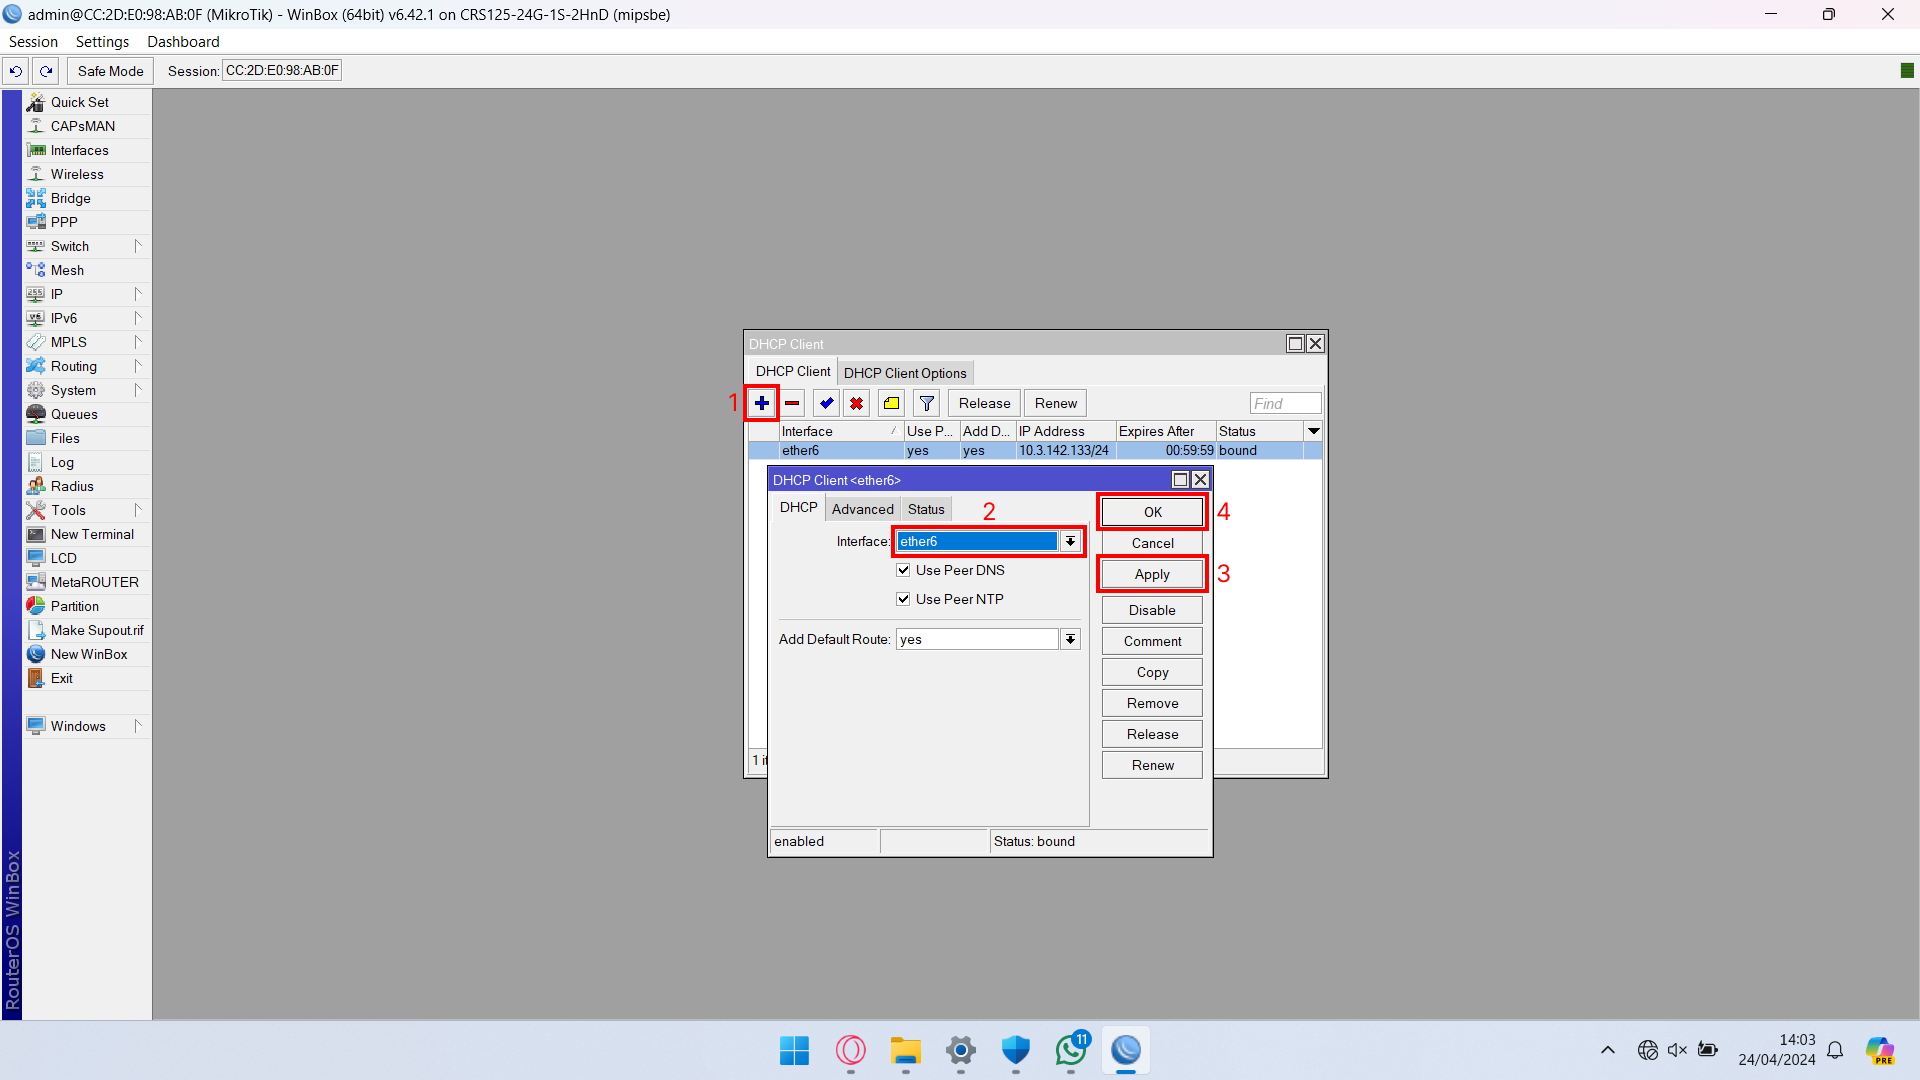
\includegraphics[width=0.8\linewidth]{P3/img/Step 2.2.png}
			\caption{Step 2.2}
			\label{fig:Step 2.2}
		\end{figure}
        \item Buat IP address pada Router yang menghubungkan PC dengan Router. Tambahkan IP address > Isi address > Pilih Interface yang terhubung ke PC (ether2) > Klik Apply > Klik OK.
        \begin{figure}[H]
			\centering
			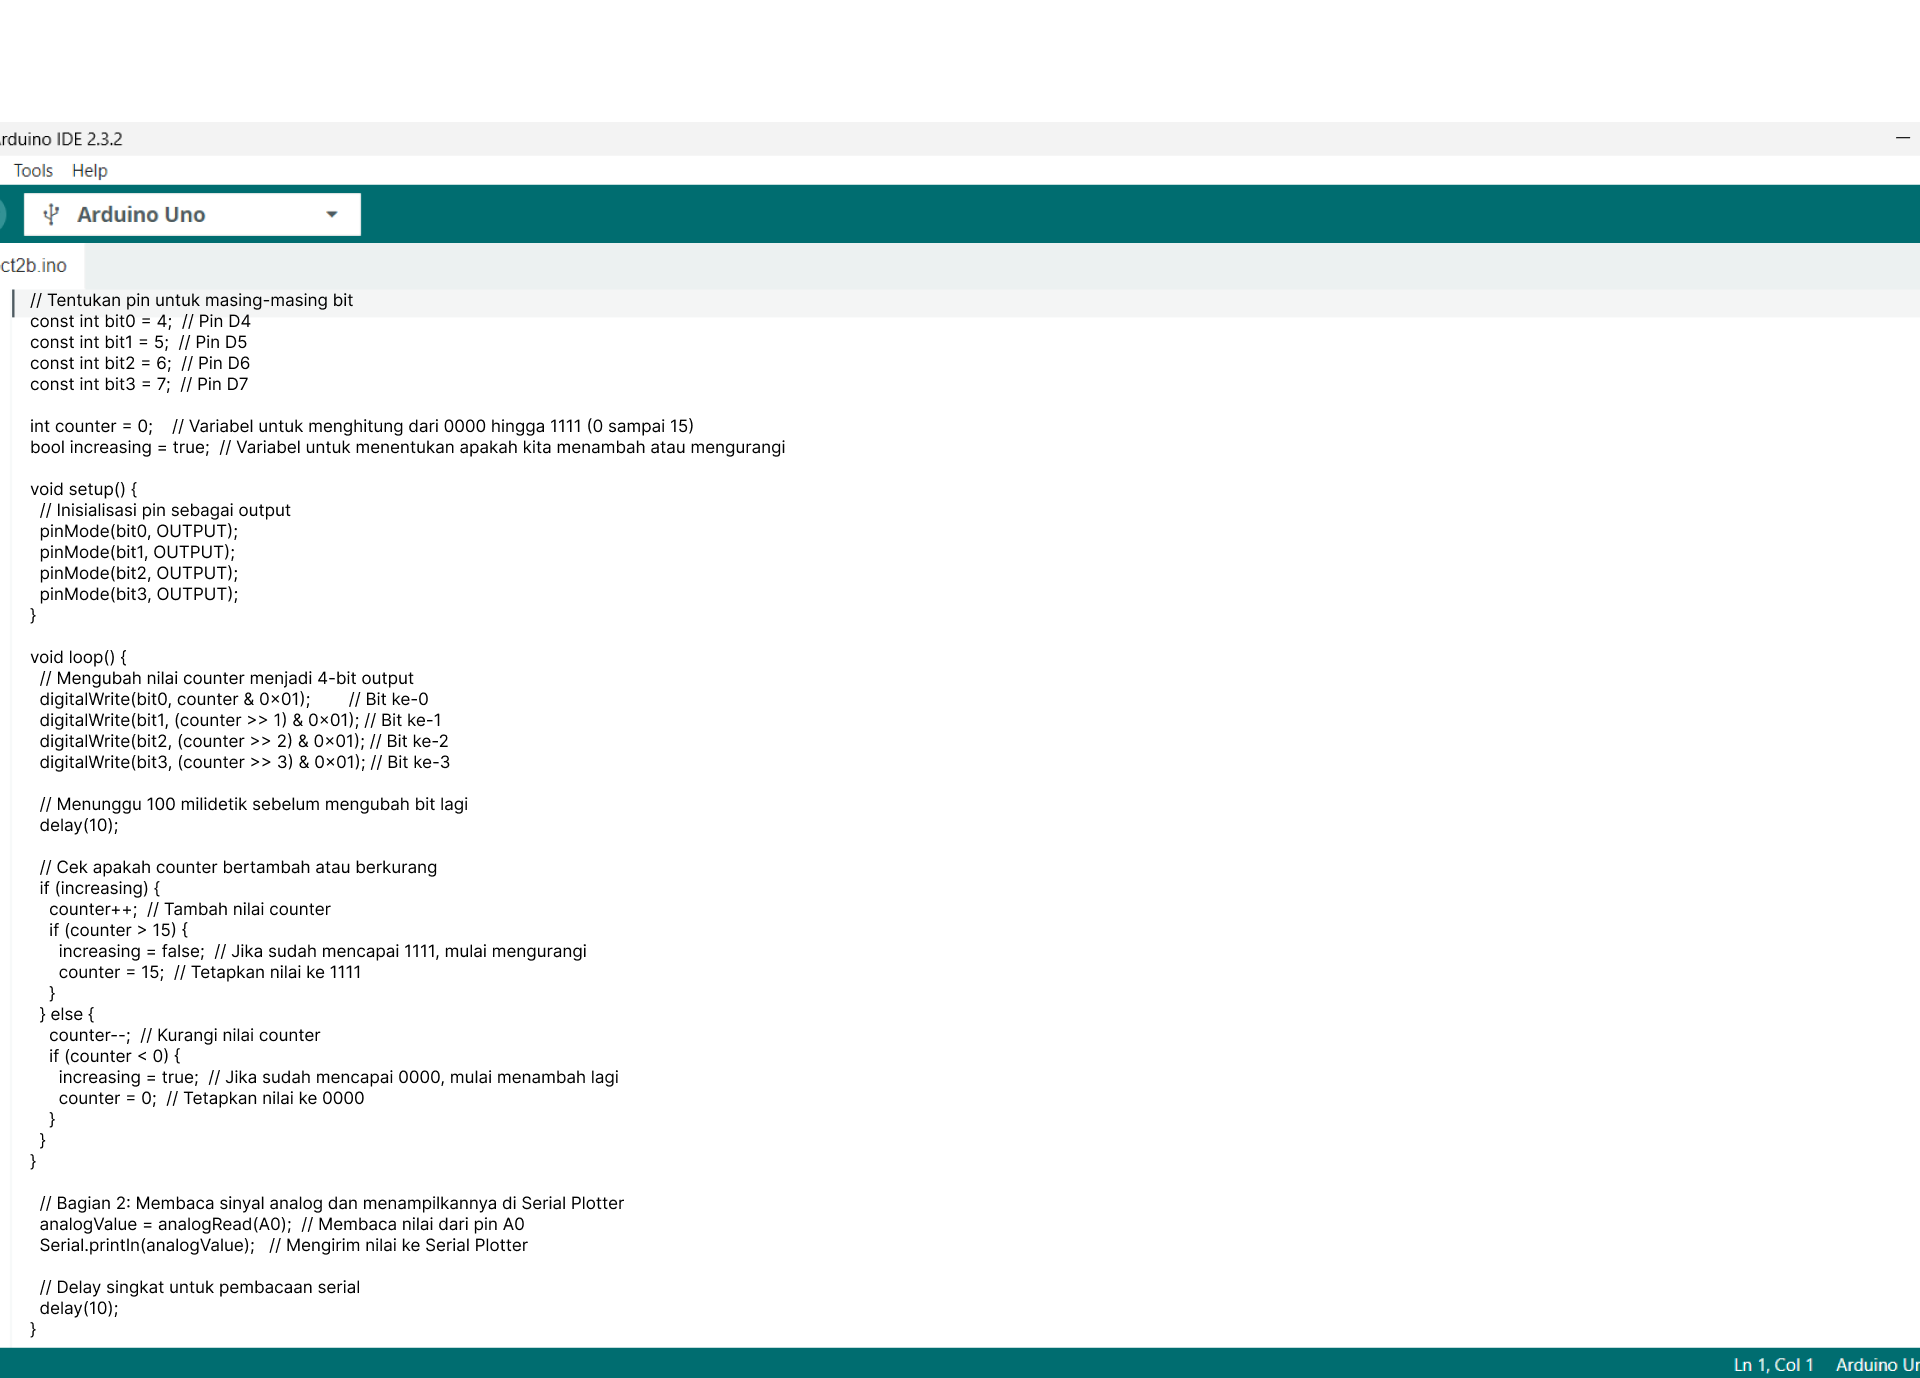
\includegraphics[width=0.8\linewidth]{P3/img/Step 3.png}
			\caption{Step 3}
			\label{fig:Step 3}
		\end{figure}
        \item Jadikan Router menjadi DHCP Server agar bisa memberikan IP address secara DInamis kepada perangkat yang akan terhubung ke Router. IP > Klik DHCP Server
        \begin{figure}[H]
			\centering
			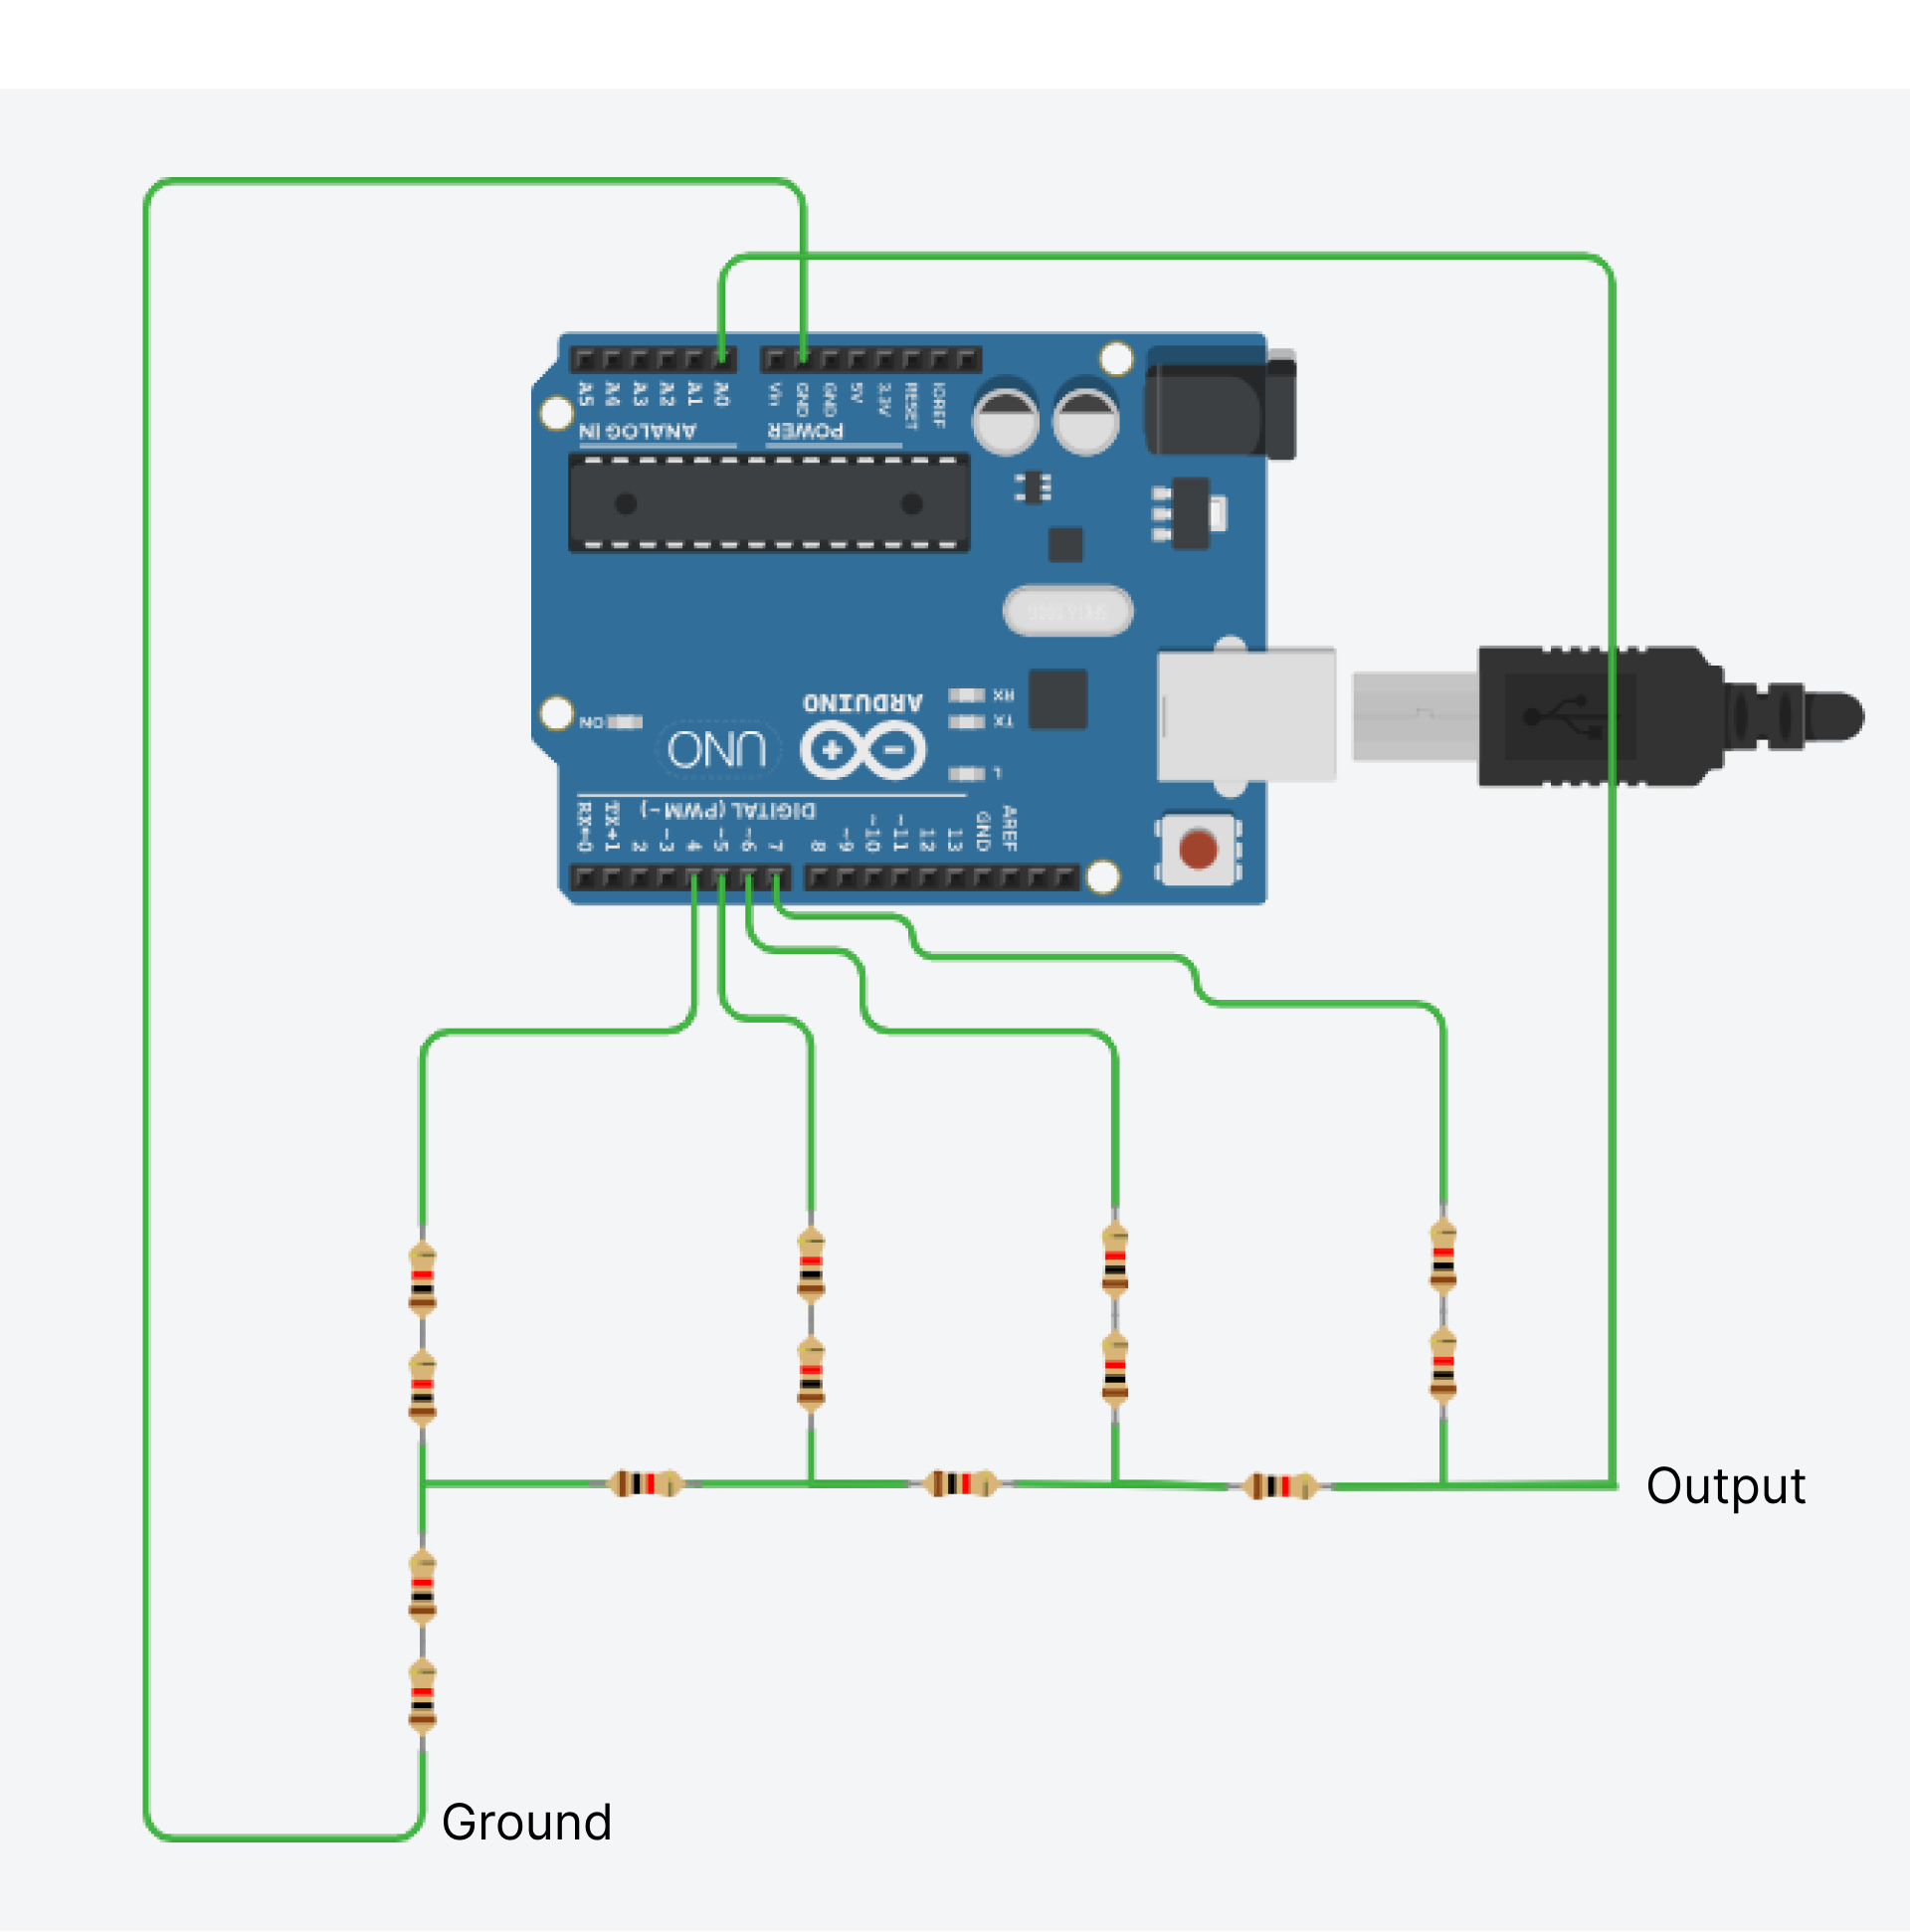
\includegraphics[width=0.8\linewidth]{P3/img/Step 4.png}
			\caption{Step 4}
			\label{fig:Step 4}
		\end{figure}
        \item Untuk menjadikan Router menjadi DHCP Server ada beberapa parameter yang harus di buat. Parameter pertama adalah DHCP Server Interface yang akan menjadi port Output DHCP Server. Klik DHCP Setup > Pilih Interface yang yang akan menjadi Server (ether2).
        \begin{figure}[H]
			\centering
			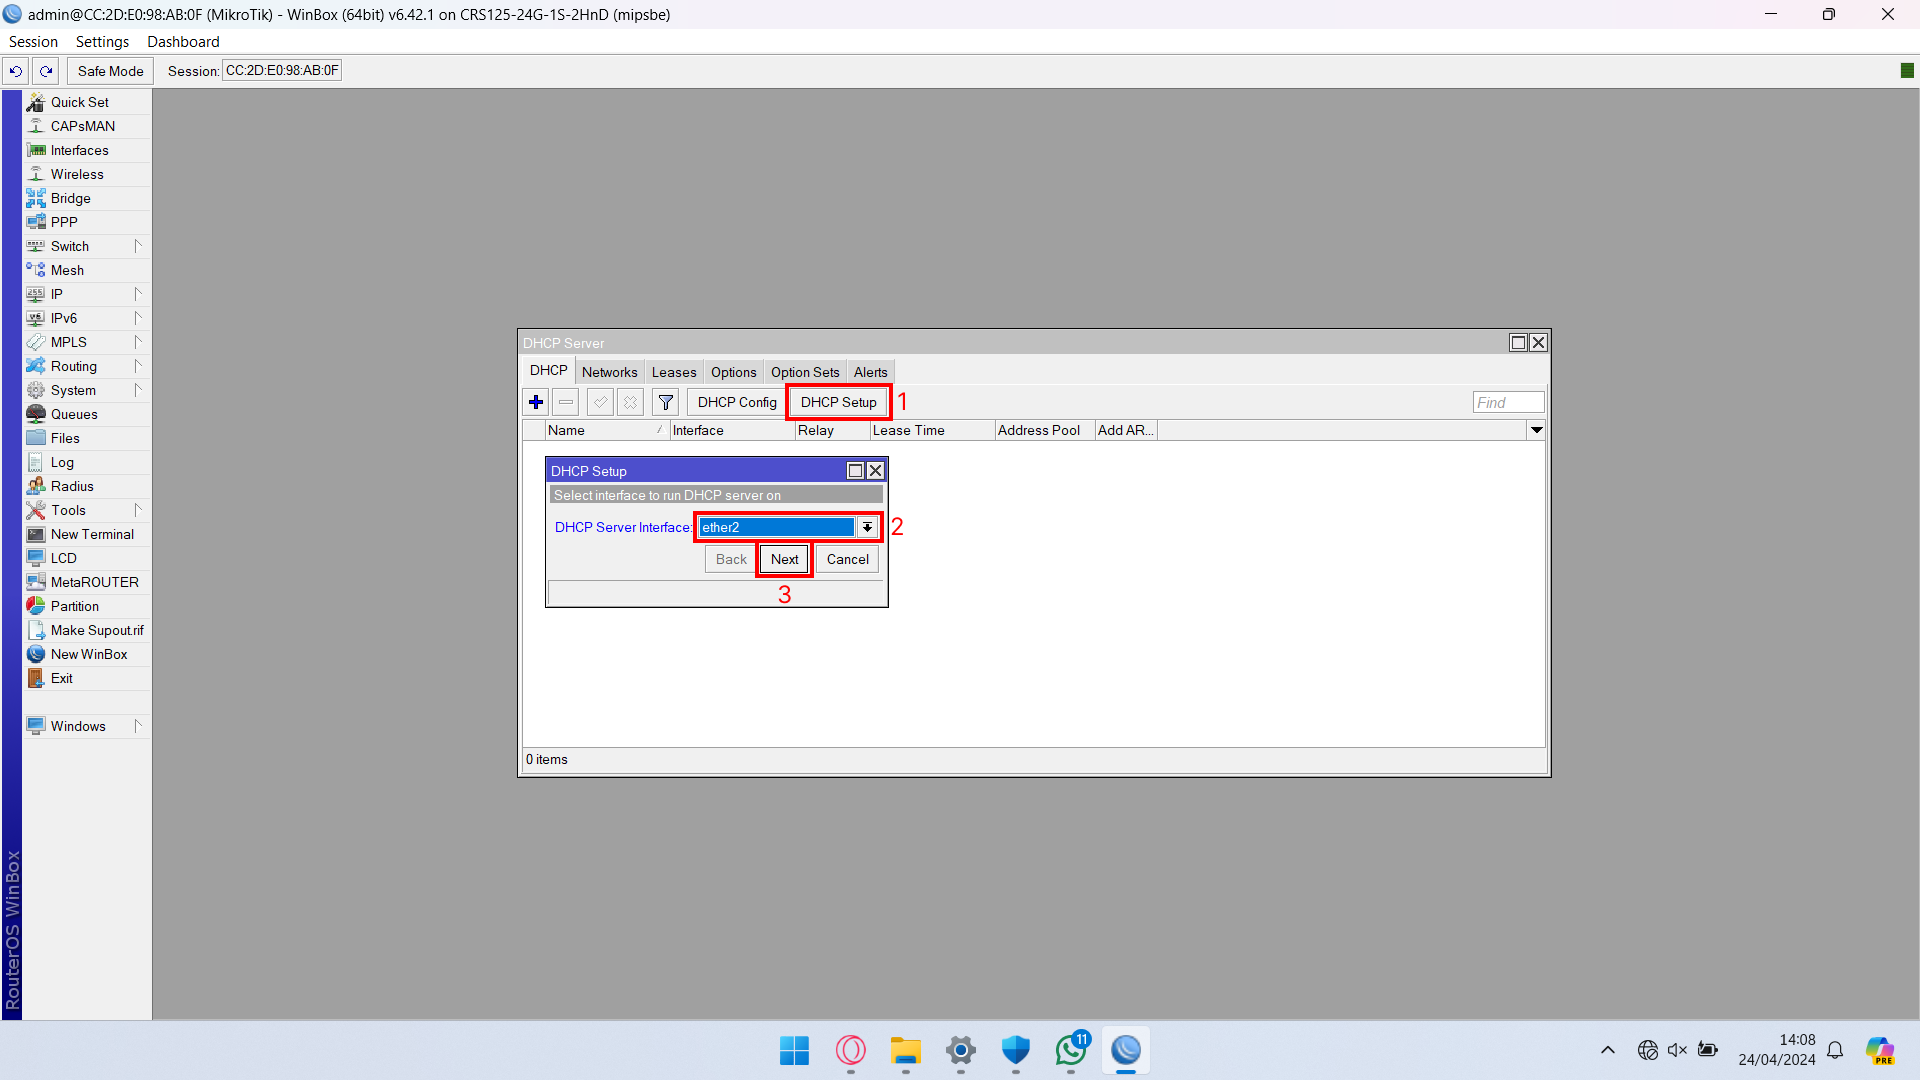
\includegraphics[width=0.8\linewidth]{P3/img/Step 5.png}
			\caption{Step 5}
			\label{fig:Step 5}
		\end{figure}
        \item Parameter kedua adalah DHCP Address Space. Isinya adalah alamat Network yang ingin dibuat. Oleh karena itu alamat IP nya diakhiri dengan angka 0.
        \begin{figure}[H]
			\centering
			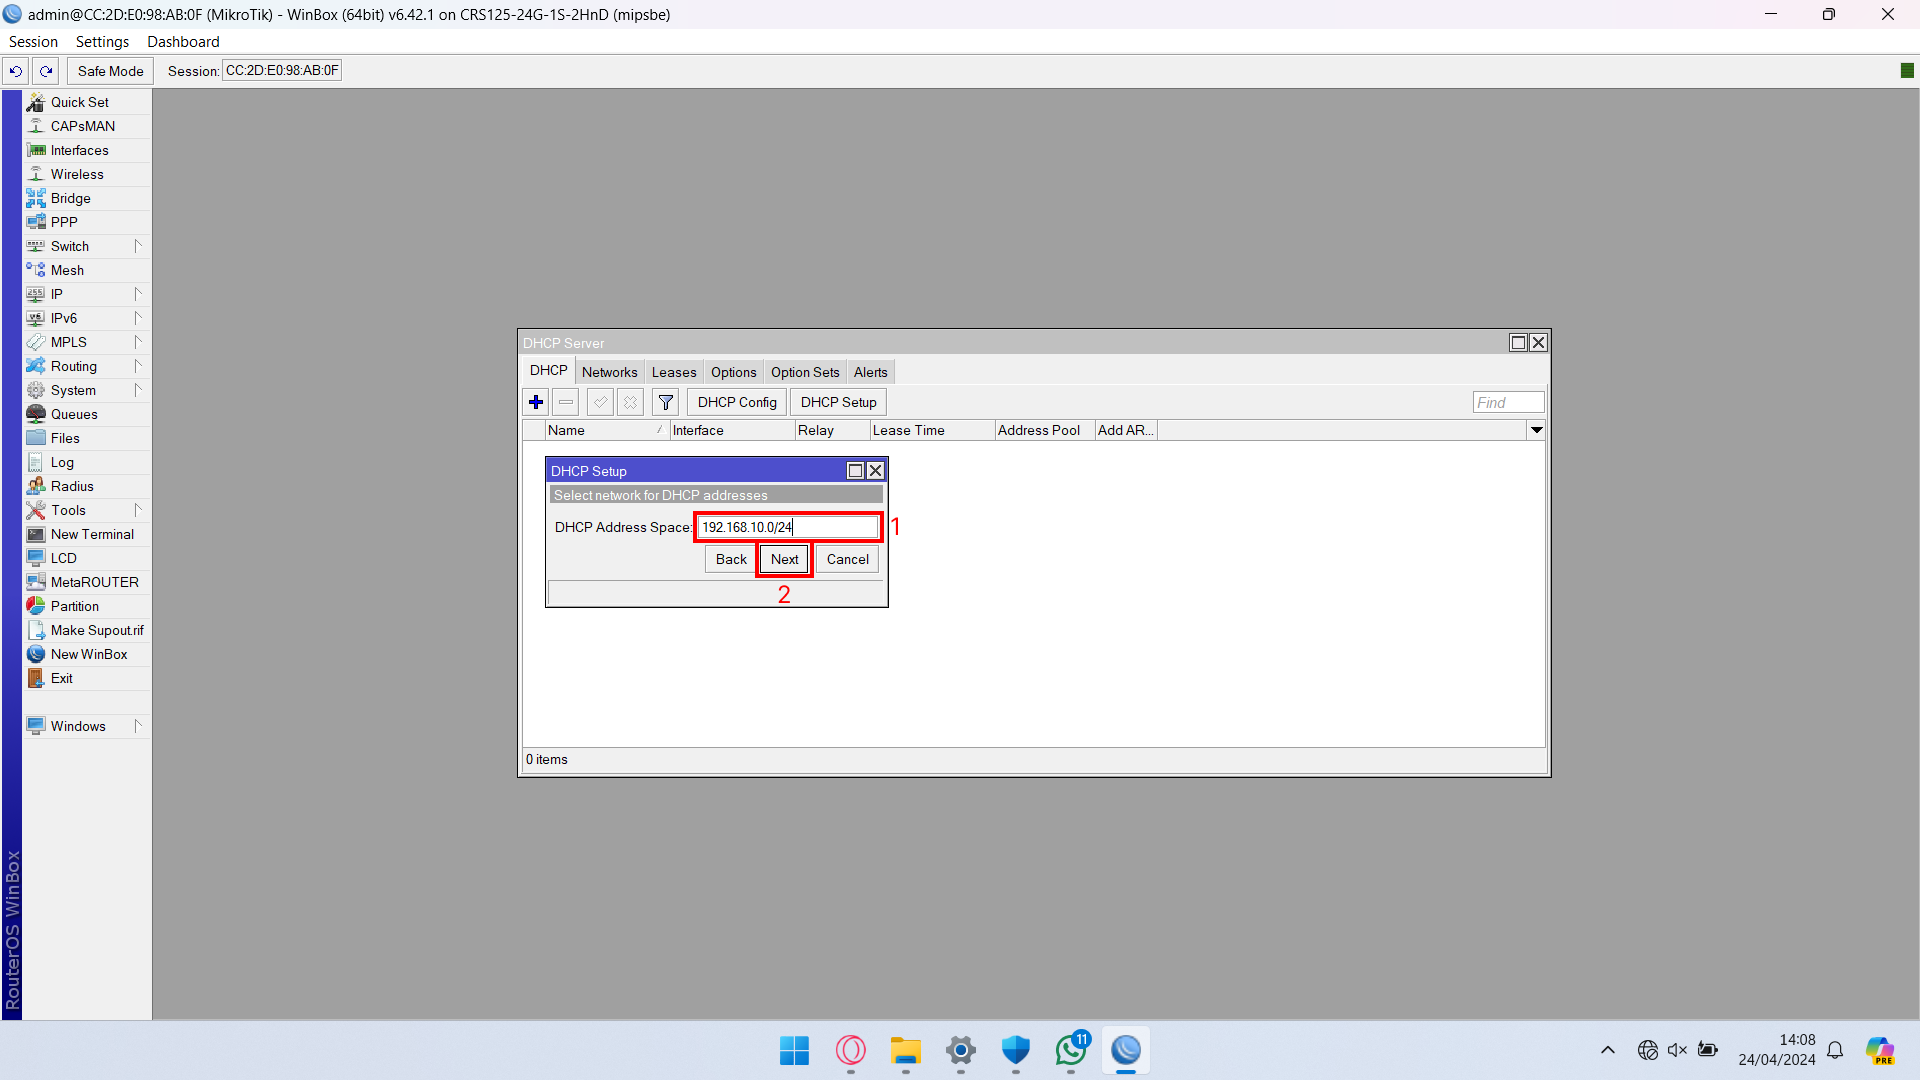
\includegraphics[width=0.8\linewidth]{P3/img/Step 6.png}
			\caption{Step 6}
			\label{fig:Step 6}
		\end{figure}
        \item Parameter ketiga adalah Gateway for DHCP Network. Isinya adalah port pada Router yang akan menghubungkan Router dengan Network address yang sudah ditentukan.
        \begin{figure}[H]
			\centering
			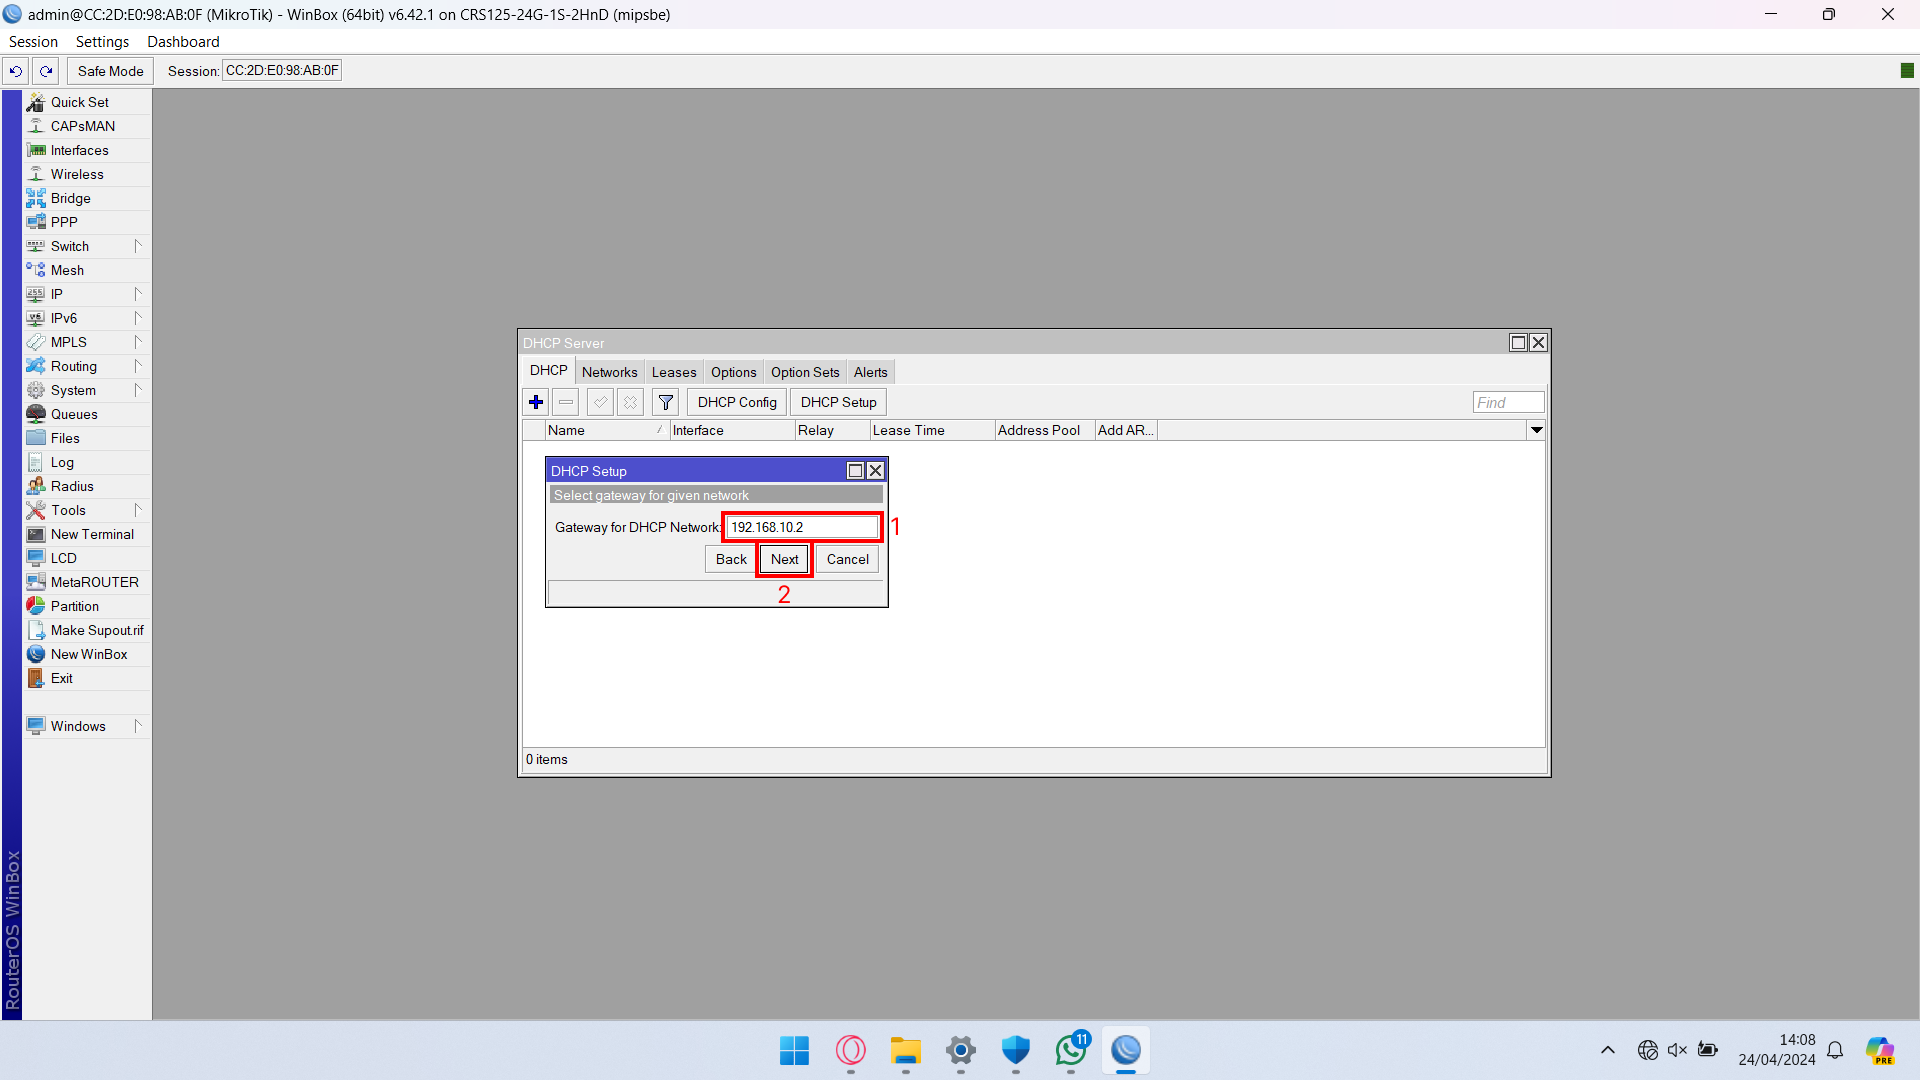
\includegraphics[width=0.8\linewidth]{P3/img/Step 7.png}
			\caption{Step 7}
			\label{fig:Step 7}
		\end{figure}
        \item Parameter keempat adalah Adresses to Give Out. Isinya adalah range IP address yang akan diberikan kepada masing-masing perangkat yang akan terhubung. Pada Modul alamat yang dapat diberikan adalah antara 192.168.10.3 sampai 192.168.10.255.
        \begin{figure}[H]
			\centering
			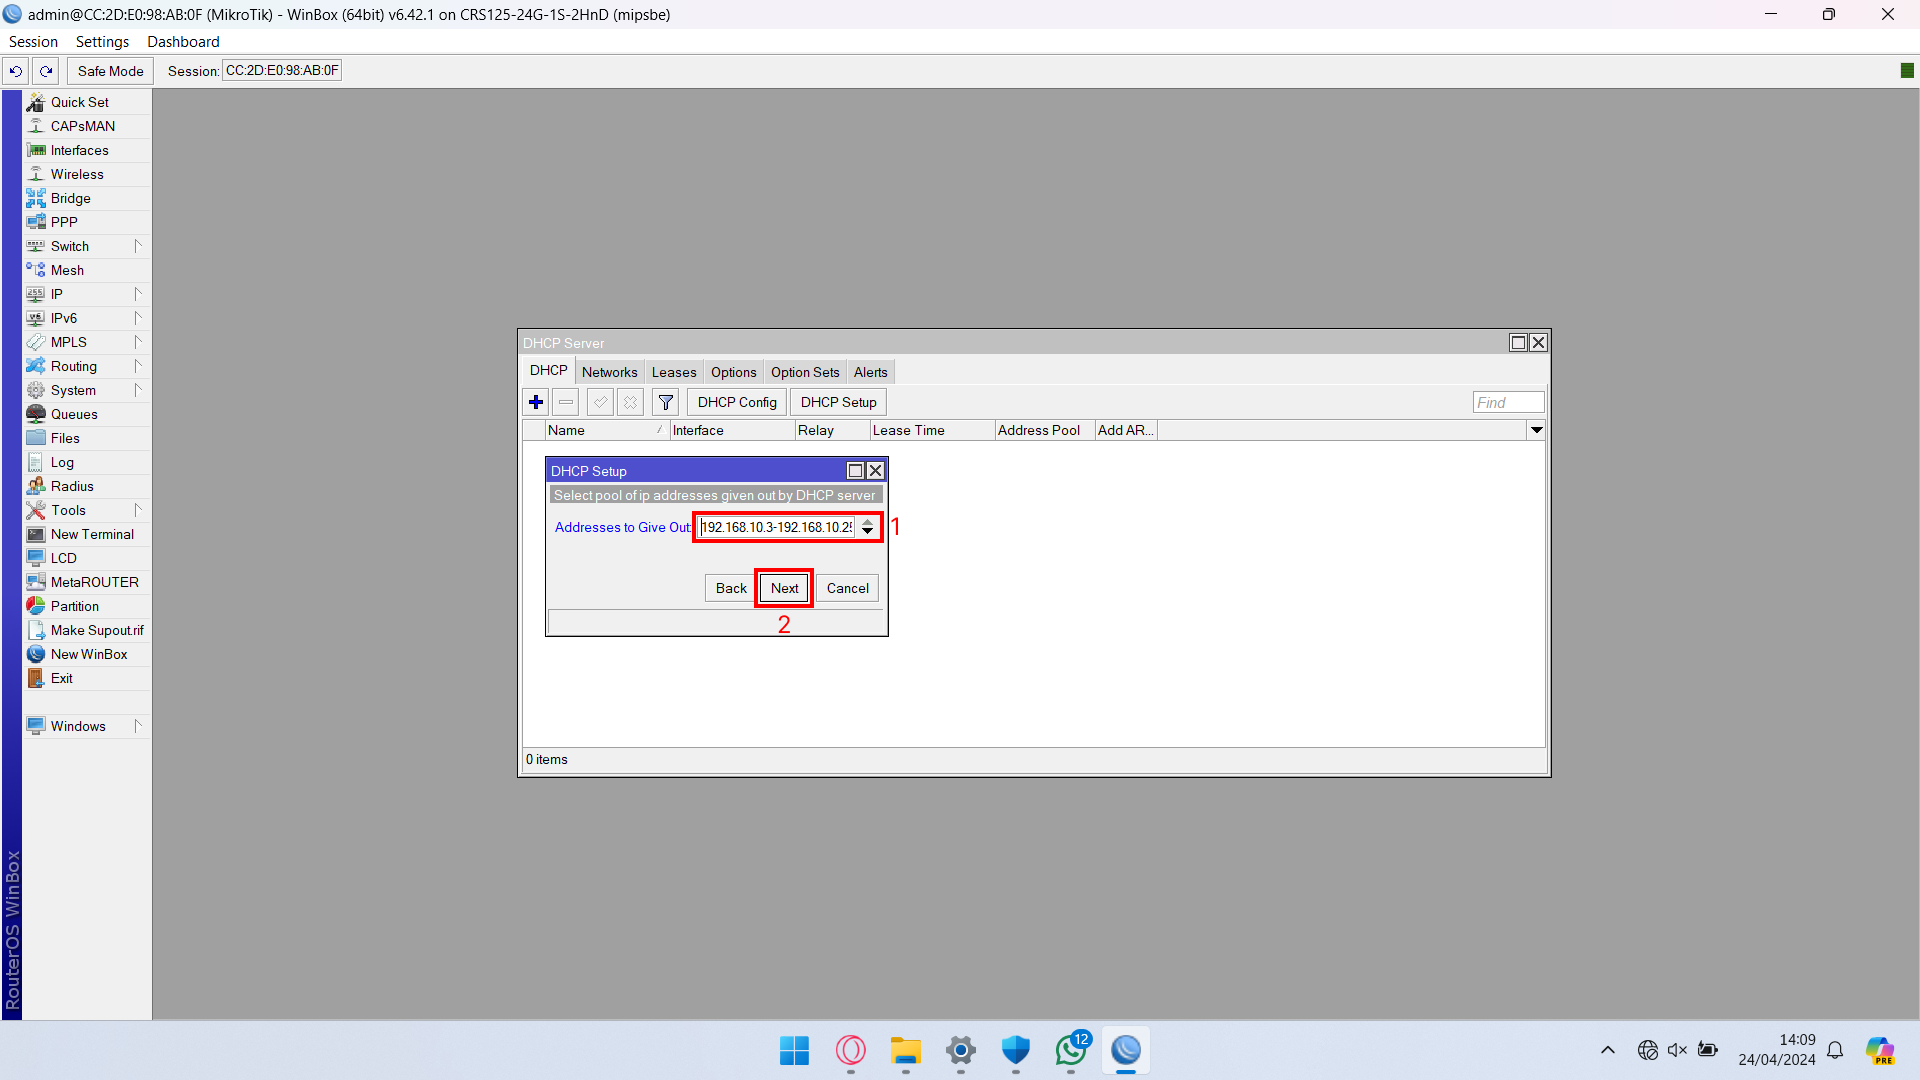
\includegraphics[width=0.8\linewidth]{P3/img/Step 8.png}
			\caption{Step 8}
			\label{fig:Step 8}
		\end{figure}
        \item Parameter kelima adalah DNS Servers. Untuk opsi langsung saja Klik Next.
        \begin{figure}[H]
			\centering
			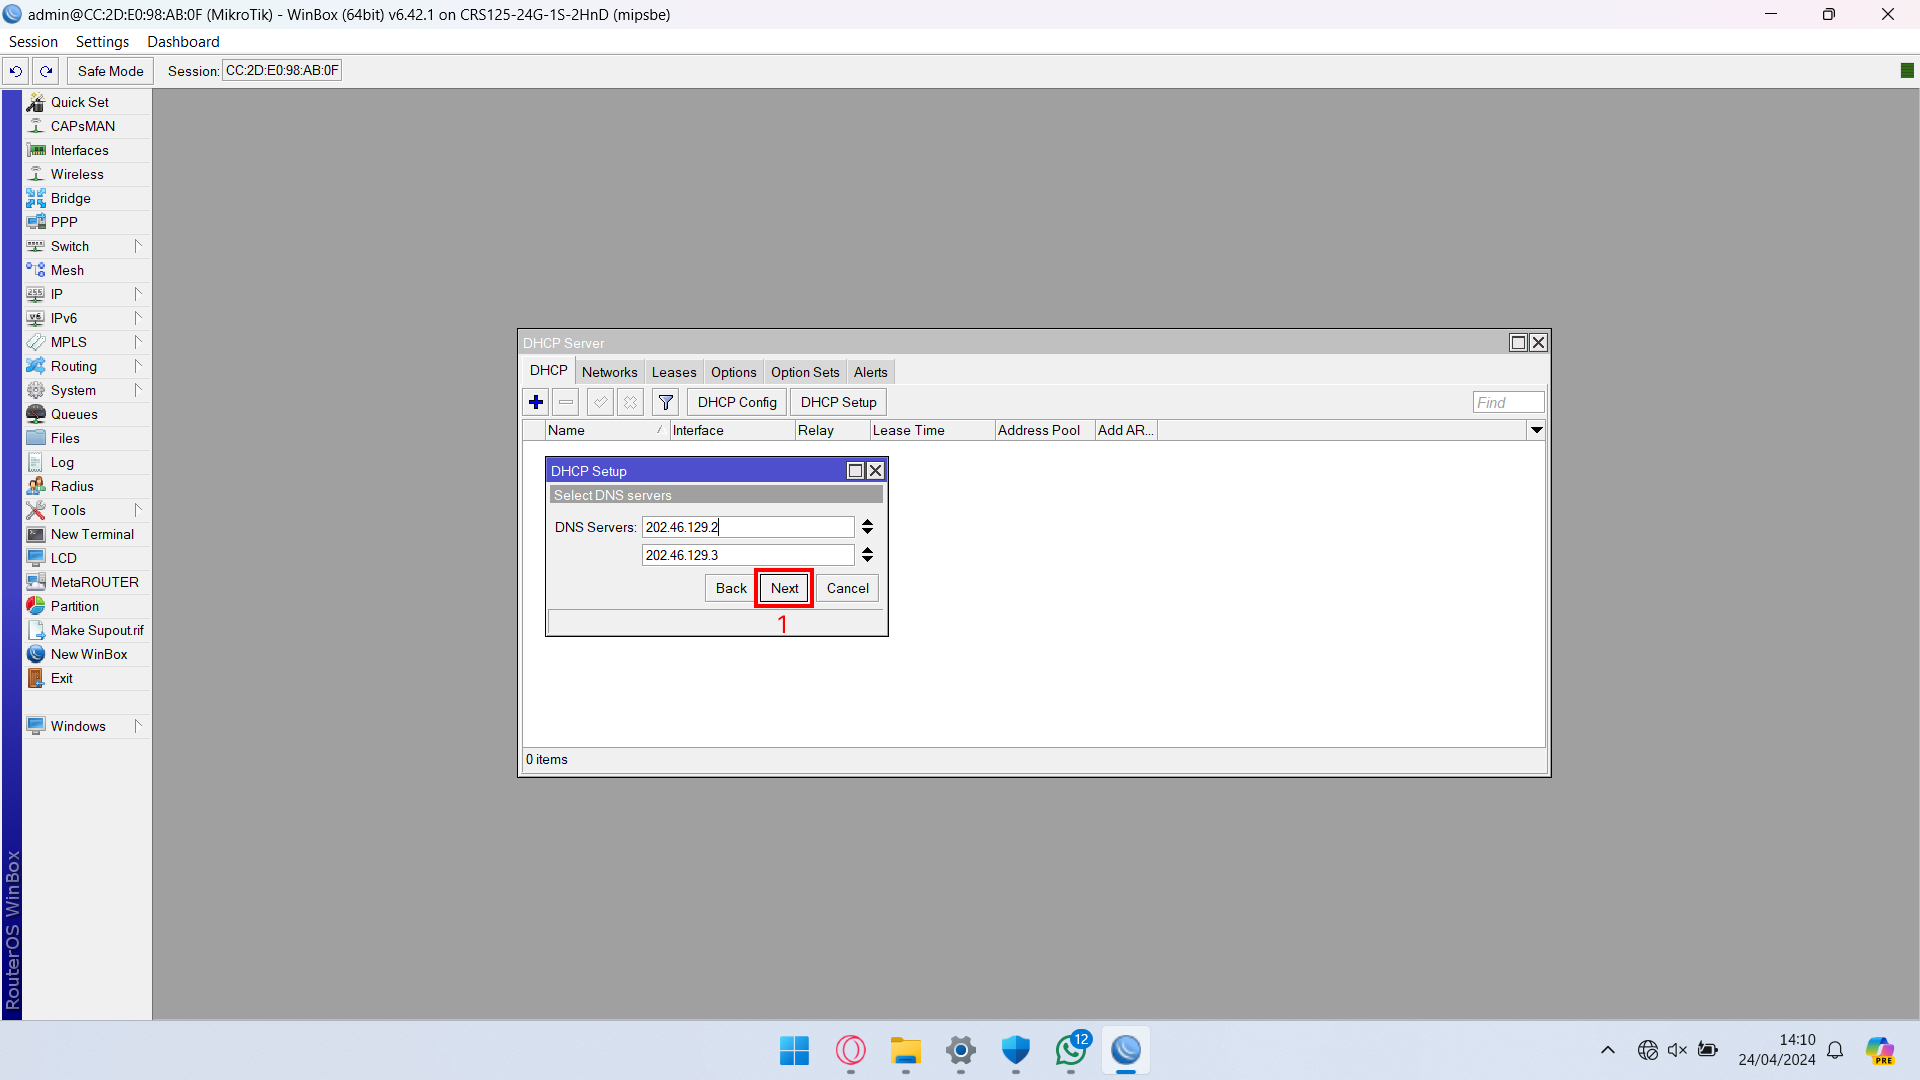
\includegraphics[width=0.8\linewidth]{P3/img/Step 9.png}
			\caption{Step 9}
			\label{fig:Step 9}
		\end{figure}
        \item Parameter keenam adalah Lease Time. Lease Time dipakai untuk membatasi waktu penggunaan IP address yang diberikan oleh Router kepada Devices. Untuk opsi langsung saja Klik Next.
        \begin{figure}[H]
			\centering
			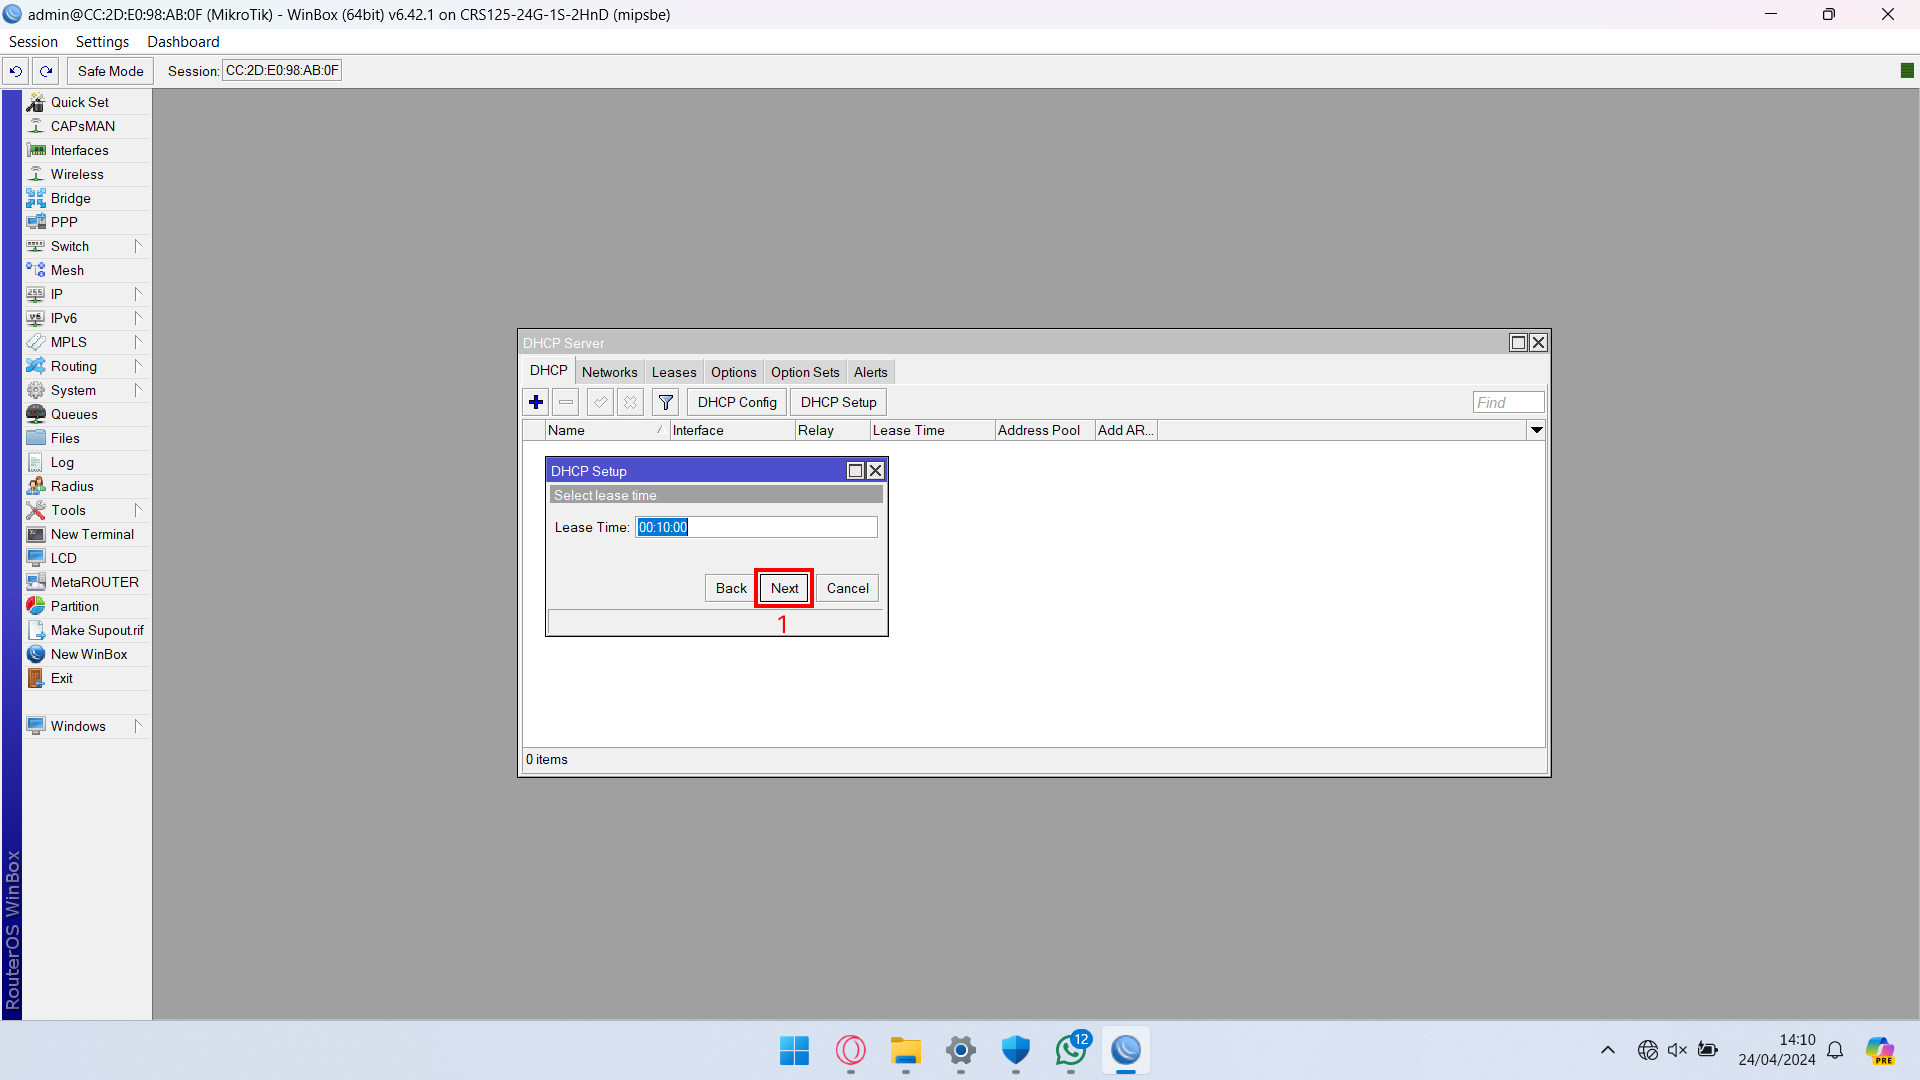
\includegraphics[width=0.8\linewidth]{P3/img/Step 10.png}
			\caption{Step 10}
			\label{fig:Step 10}
		\end{figure}
        \item Pastikan IP Settings untuk koneksi Ethernet pada PC sudah pada Mode Automatic (DHCP).
        \begin{figure}[H]
			\centering
			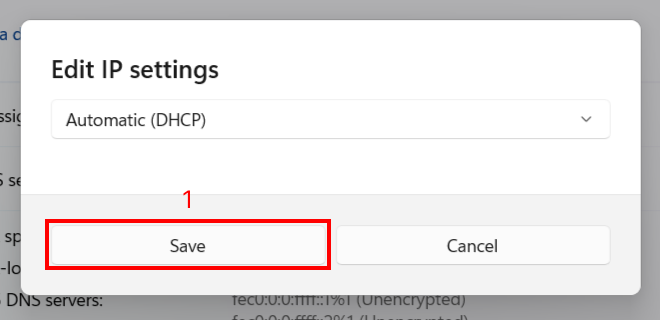
\includegraphics[width=0.8\linewidth]{P3/img/Step 11.png}
			\caption{Step 11}
			\label{fig:Step 11}
		\end{figure}
        \item Agar PC yang berada pada jaringan lokal dapat terhubung ke jaringan publik, dapat digunakan layanan NAT (Network Address Translation) yang akan menerjemahkan IP lokal beserta port perangkat agar dapat terhubung dengan jaringan publik. IP > Klik Firewall.
        \begin{figure}[H]
			\centering
			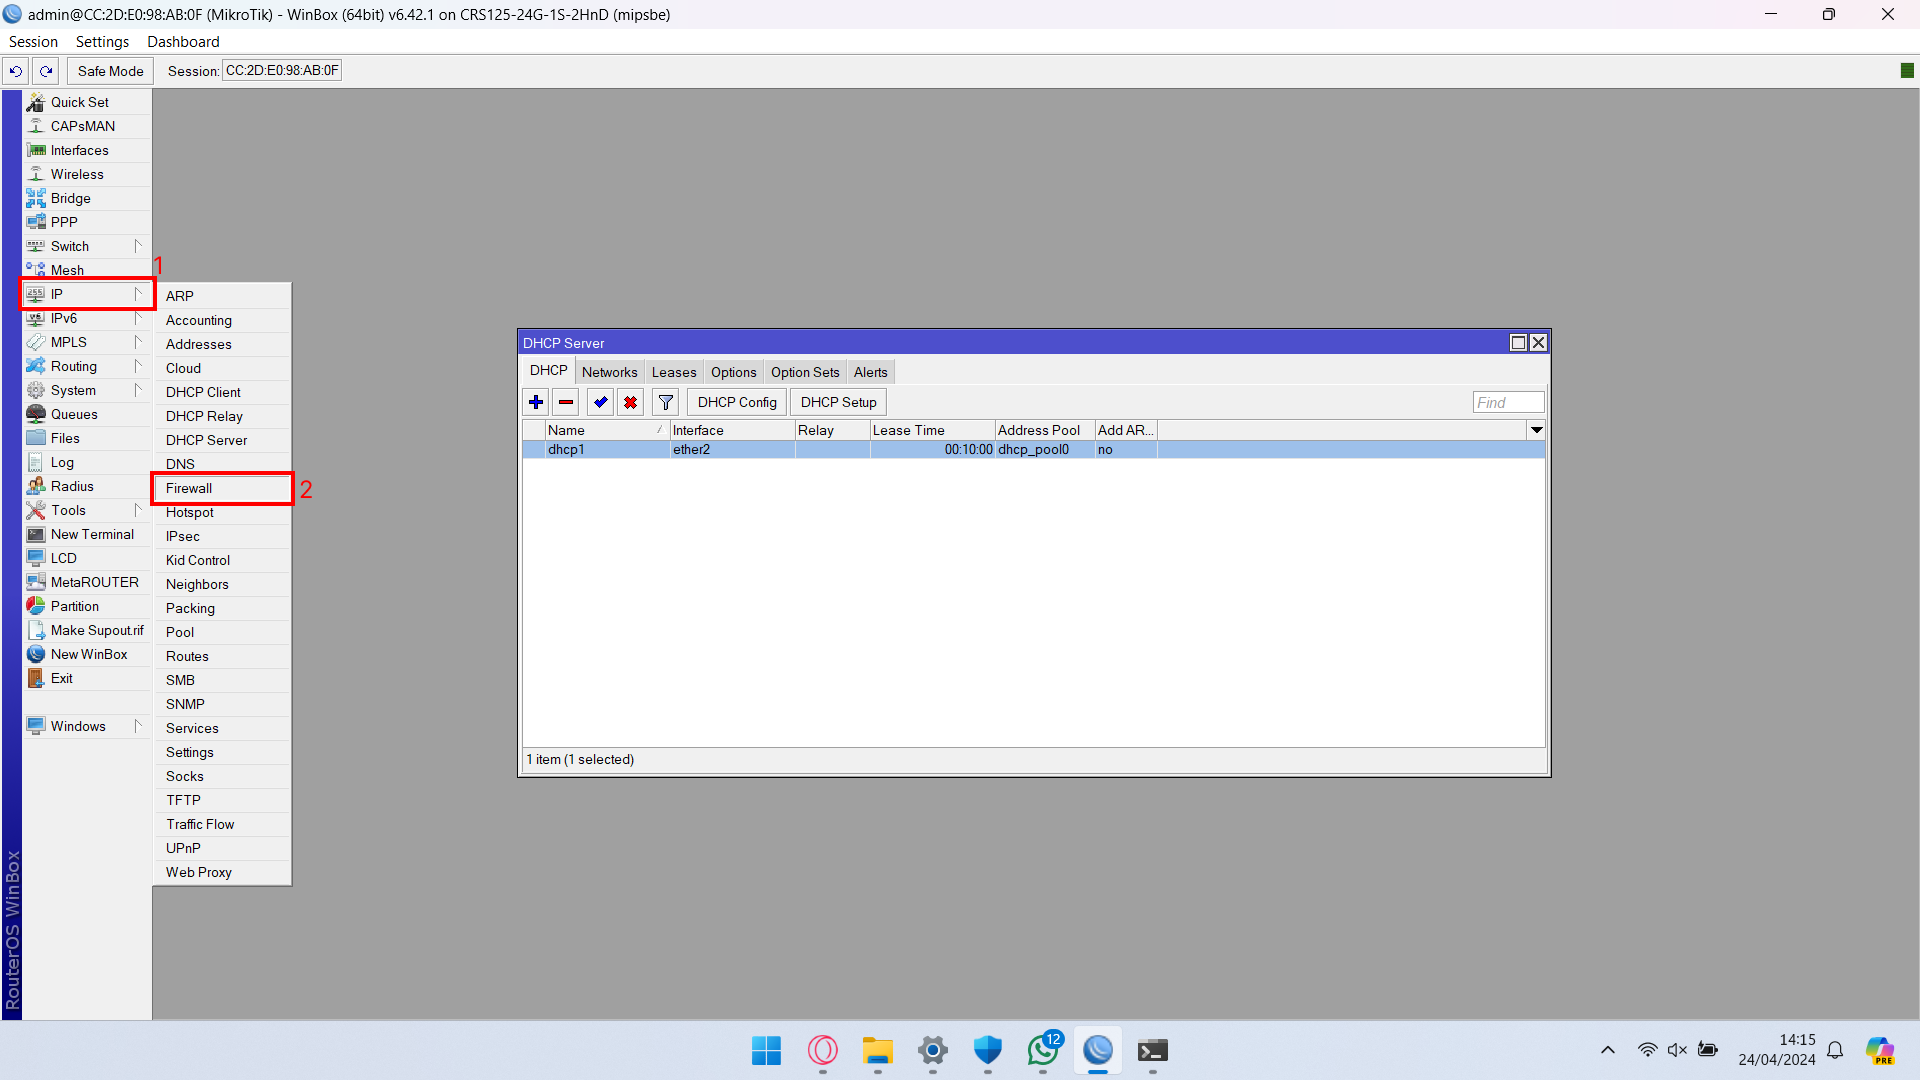
\includegraphics[width=0.8\linewidth]{P3/img/Step 12.png}
			\caption{Step 12}
			\label{fig:Step 12}
		\end{figure}
        \item Buat NAT baru. Klik tab NAT > Tambahkan NAT > Pada Opsi Chain pilih srcnat > Pilih Out Interface yaitu port pada Router yang terhubung dengan Internet(ether6) > Klik Apply. Tambahkan Action pada tab Action. Pada Opsi Action pilih masquerade > Klik Apply > Klik OK.
        \begin{figure}[H]
			\centering
			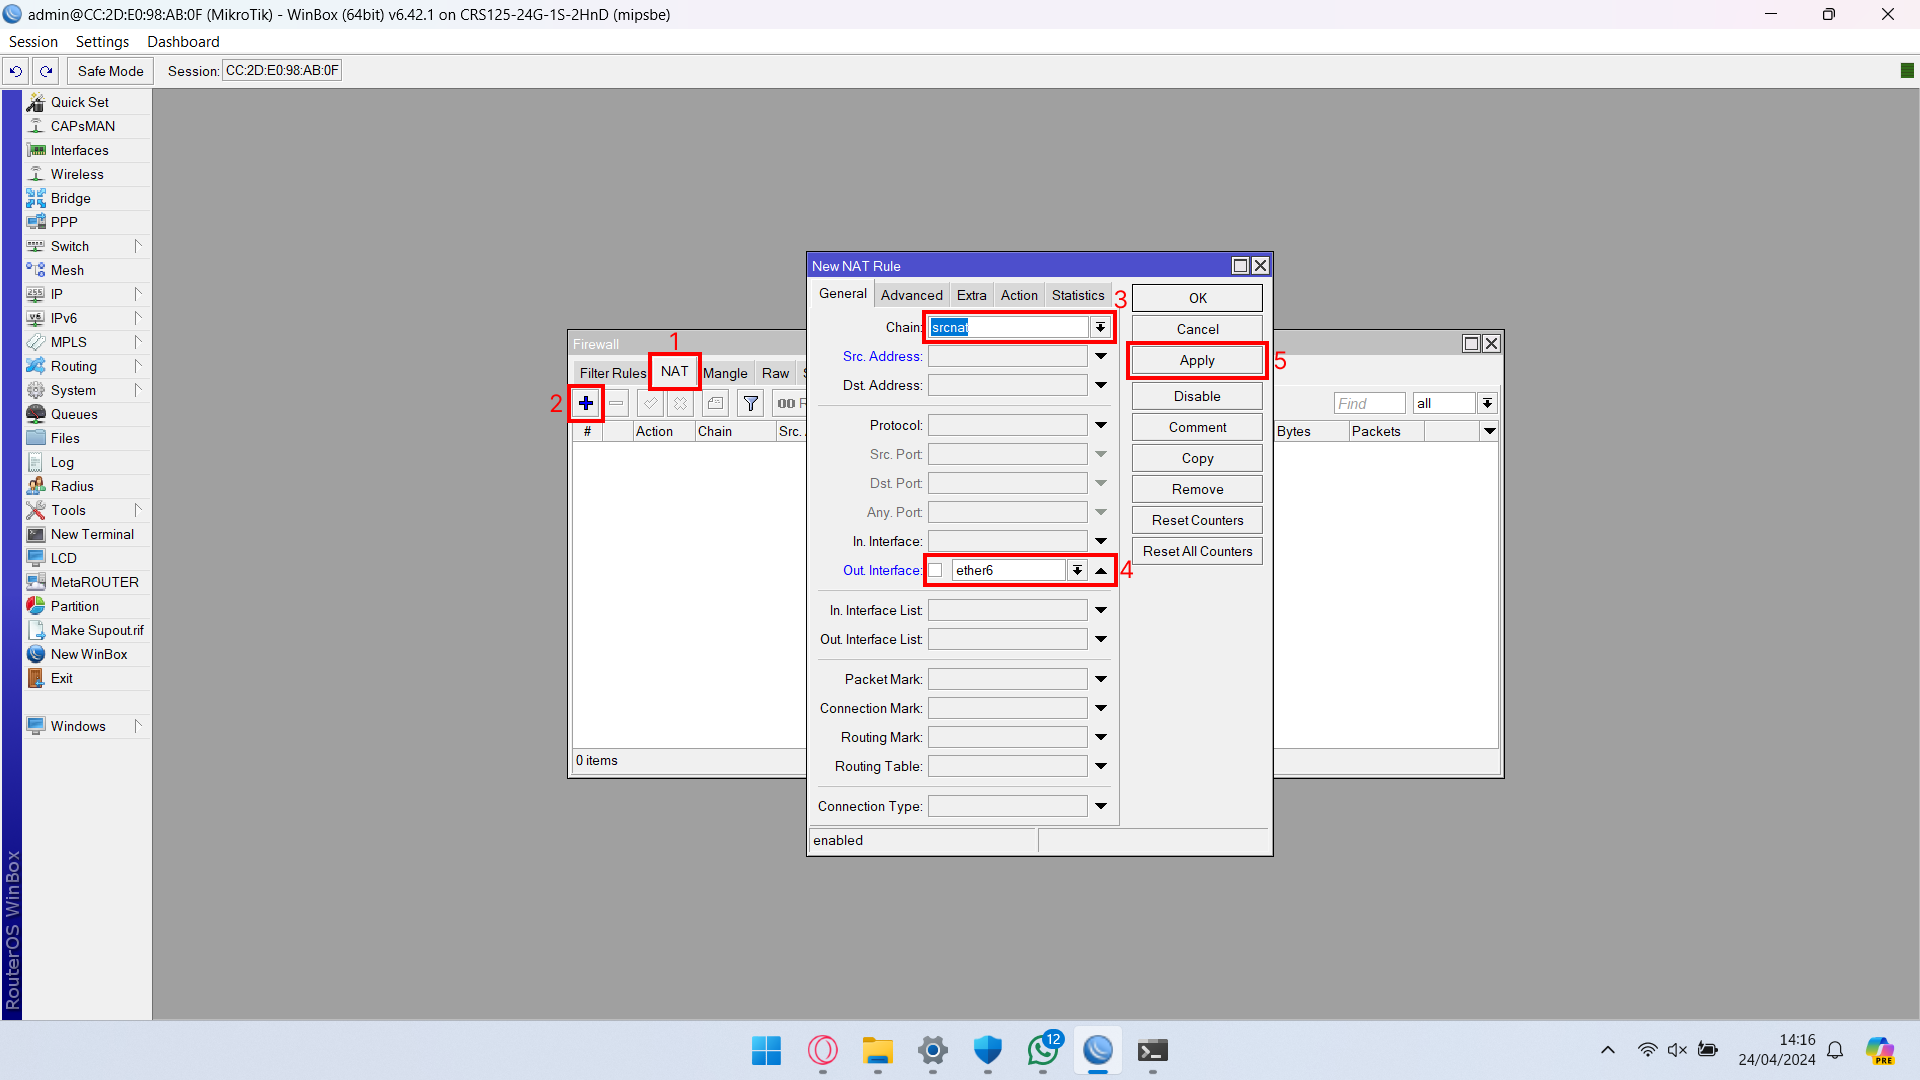
\includegraphics[width=0.8\linewidth]{P3/img/Step 13.png}
			\caption{Step 13.1}
			\label{fig:Step 13.1}
		\end{figure}
        \begin{figure}[H]
			\centering
			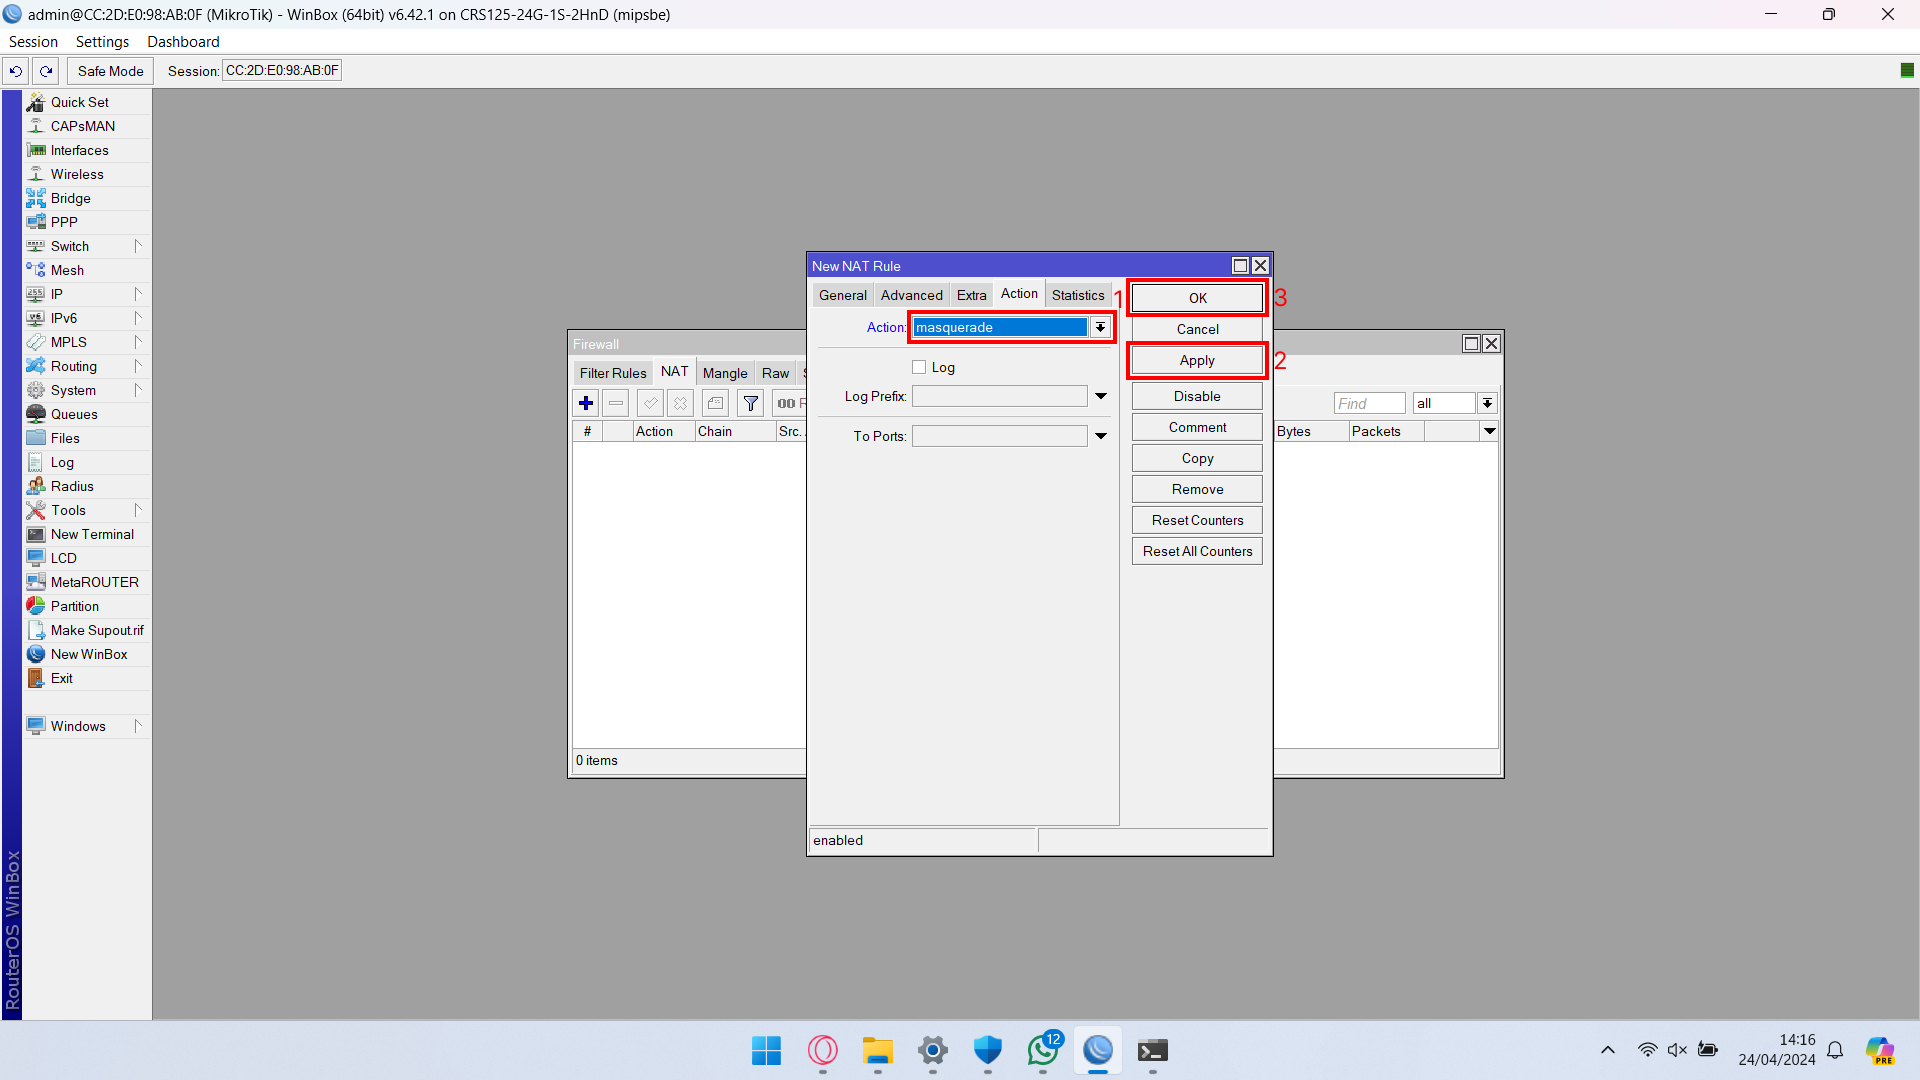
\includegraphics[width=0.8\linewidth]{P3/img/Step 14.png}
			\caption{Step 13.2}
			\label{fig:Step 14.2}
		\end{figure}
        \item Lakukan test ping ke 8.8.8.8 untuk memastikan PC sudah terhubung dengan jaringan luar.
        \begin{figure}[H]
			\centering
			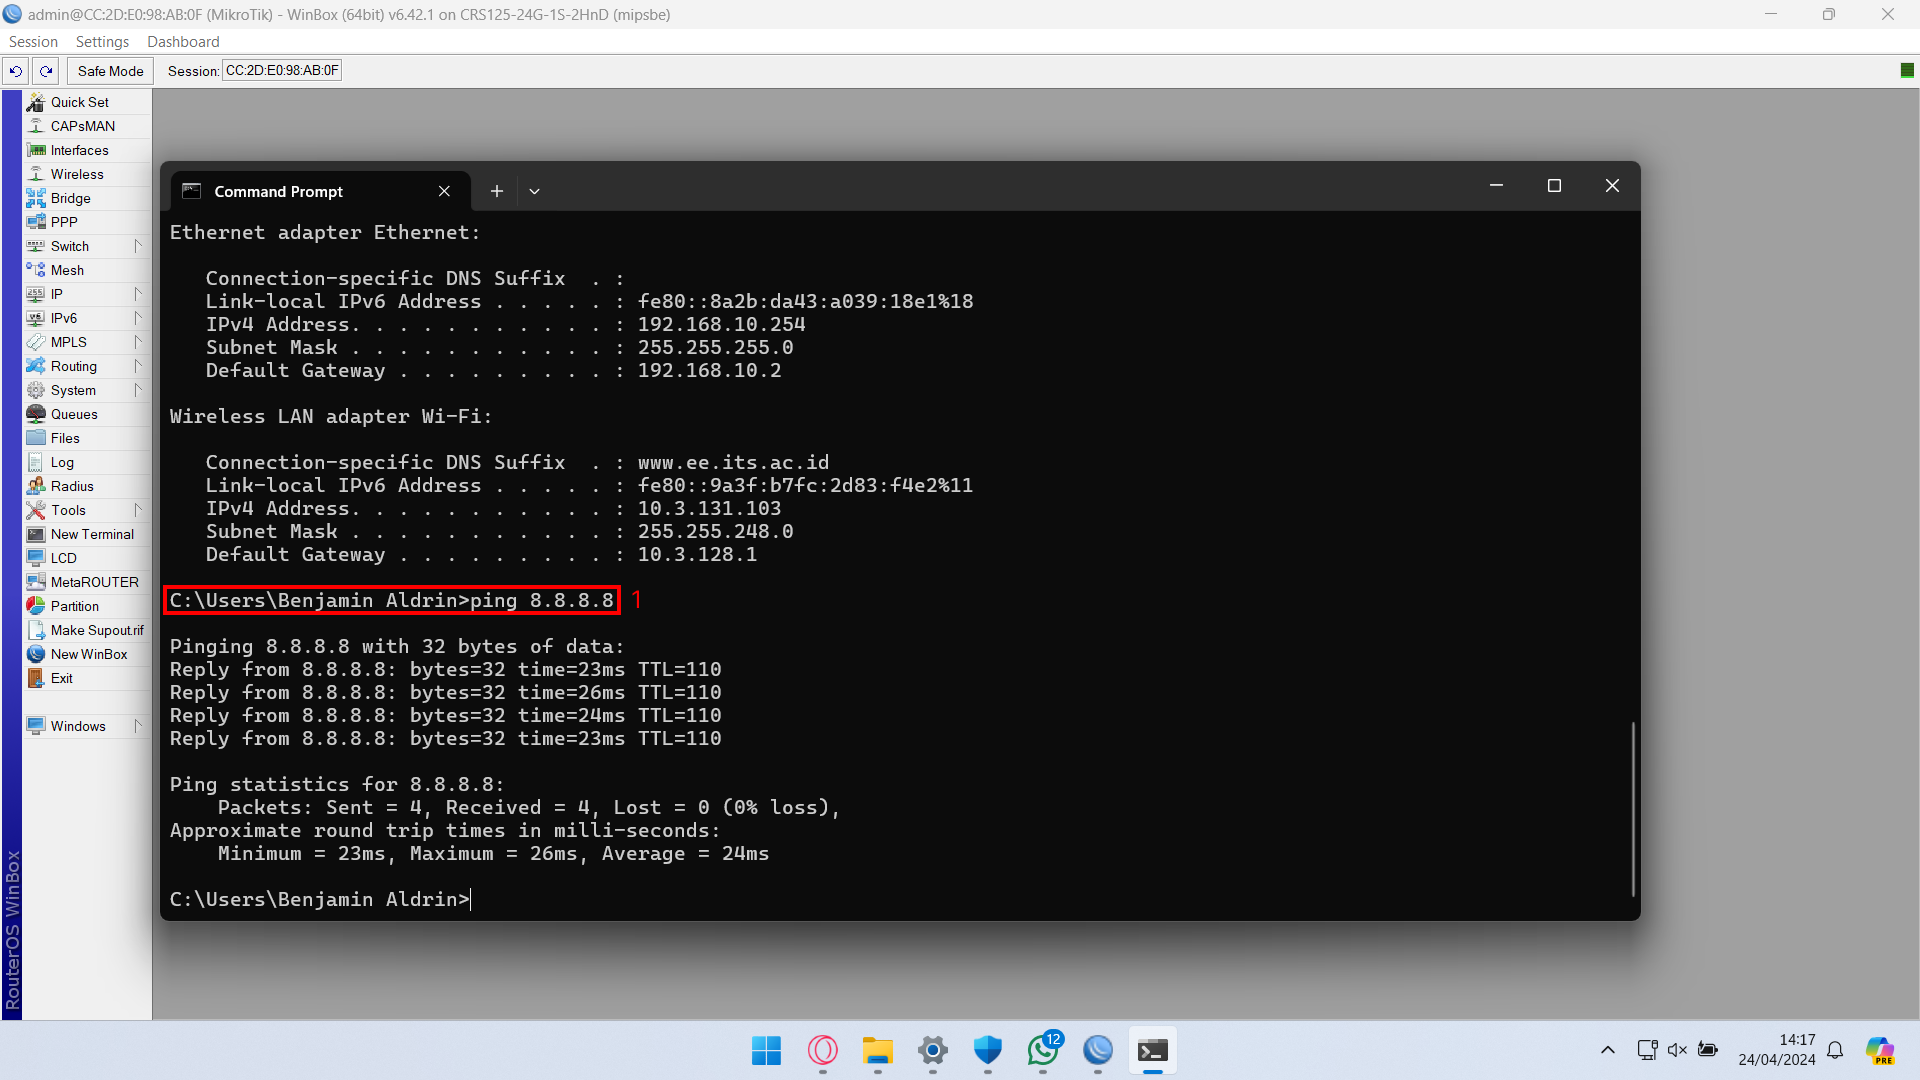
\includegraphics[width=0.8\linewidth]{P3/img/Step 15.png}
			\caption{Step 14}
			\label{fig:Step 14}
		\end{figure}
        \item Lakukan test bandwidth menggunakan SPEEDTEST melalui search engine PC.
        \begin{figure}[H]
			\centering
			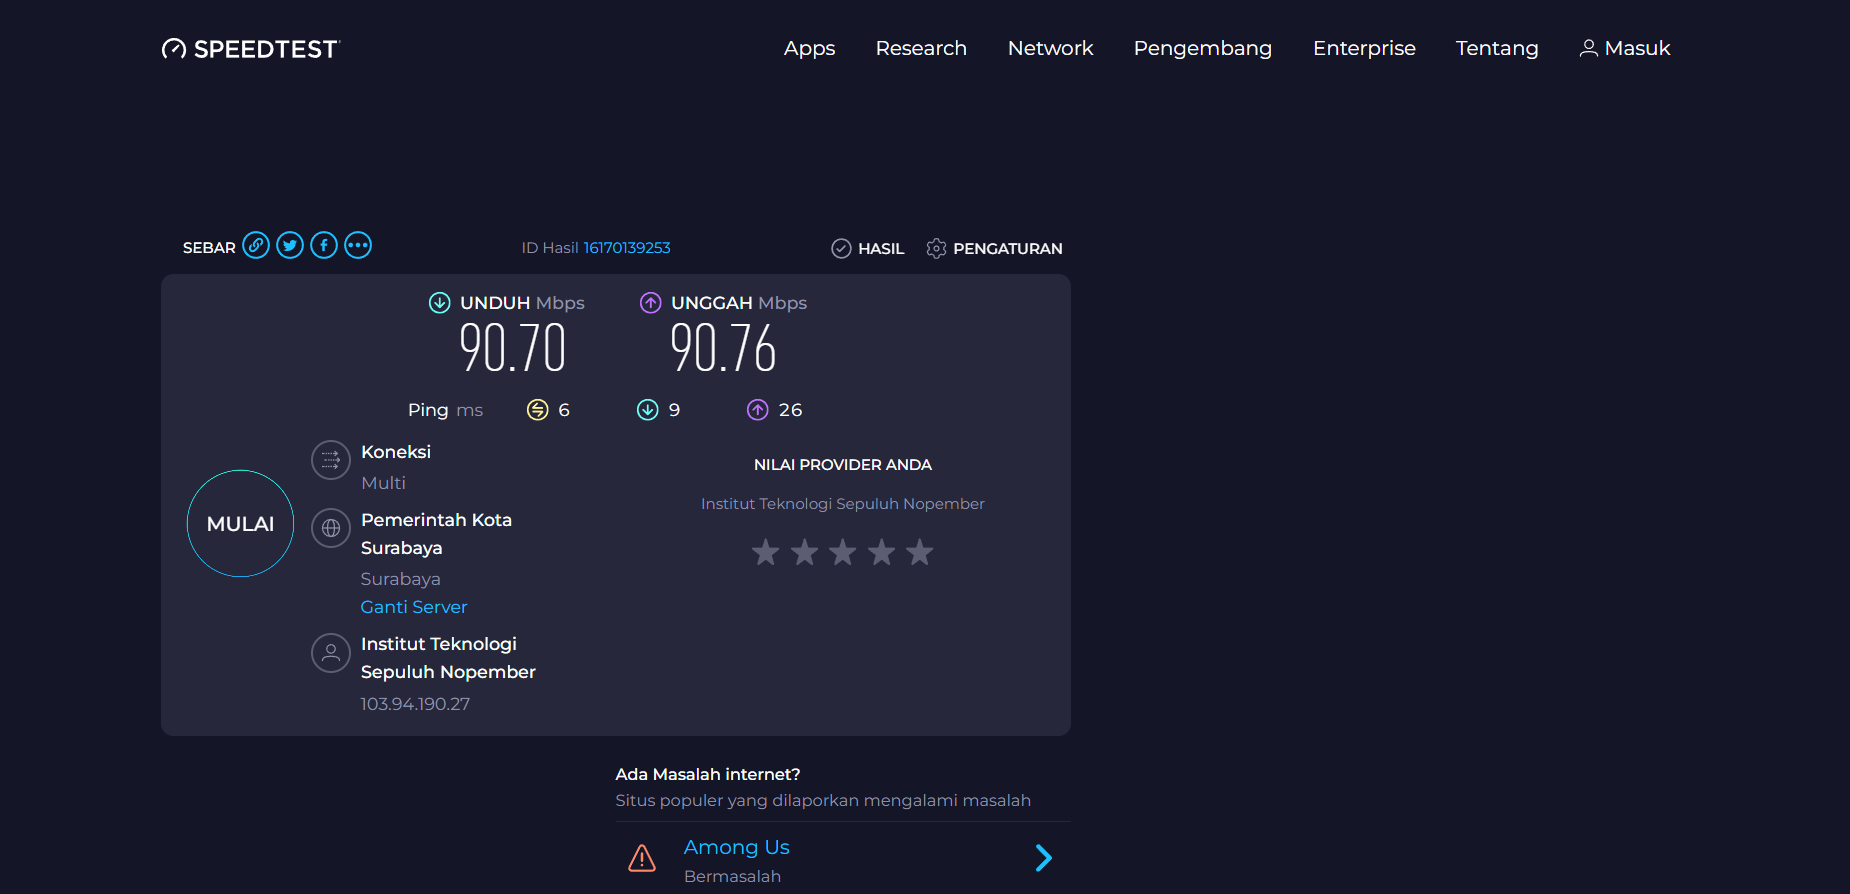
\includegraphics[width=0.8\linewidth]{P3/img/Step 16.png}
			\caption{Step 15}
			\label{fig:Step 15}
		\end{figure}
        \item Lakukan pembatasan bandwidht menggunakan Queues. Klik Queues,  Klik Queues > Tambahkan Queue List > Isi Nama perangkat yang ingin dibatasi bandwidthnya > Isi target dengan IP address PC (dapat dilihat melalui ipconfig) > Batasi Target Uploadnya menjadi 1M > Batasi Target Downloadnya menjadi 1M > Klik Apply > Klik OK.
        \begin{figure}[H]
			\centering
			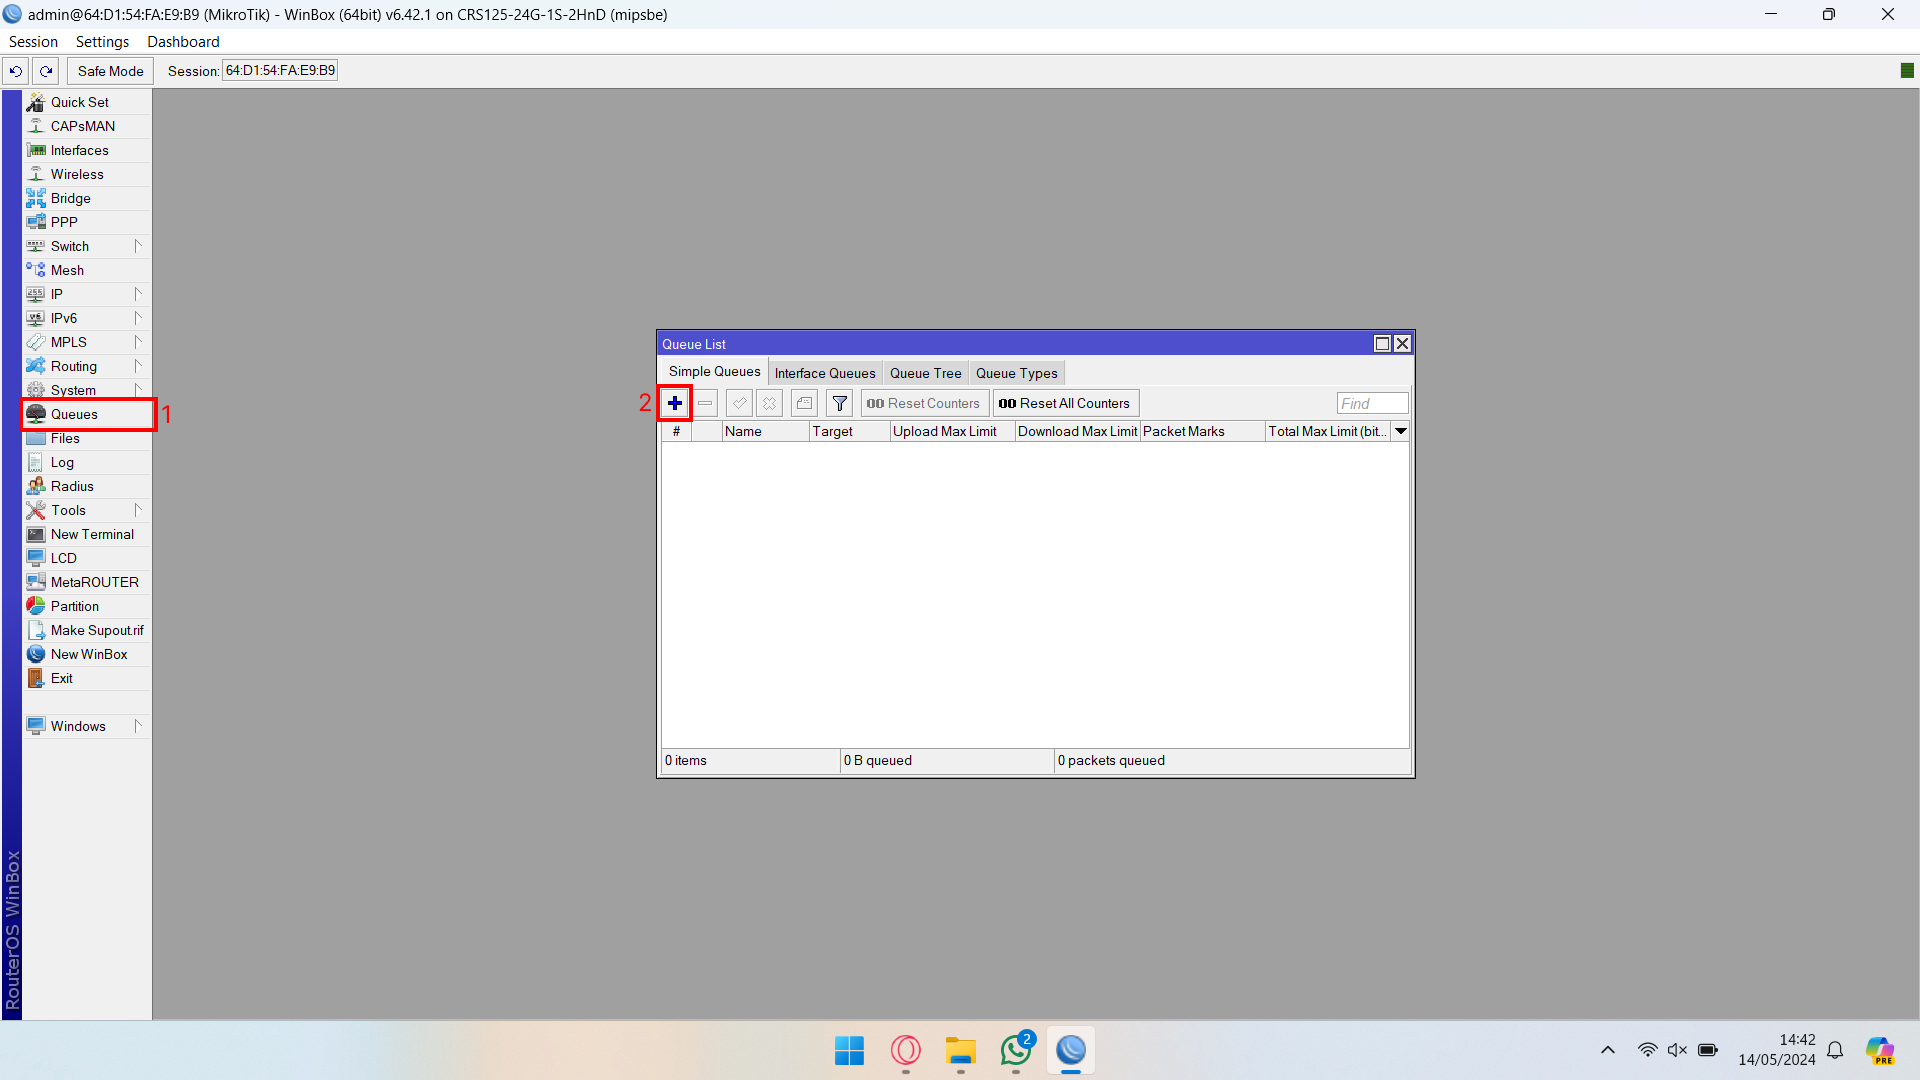
\includegraphics[width=0.8\linewidth]{P3/img/Step 17.png}
			\caption{Step 16.1}
			\label{fig:Step 16.1}
		\end{figure}
        \begin{figure}[H]
			\centering
			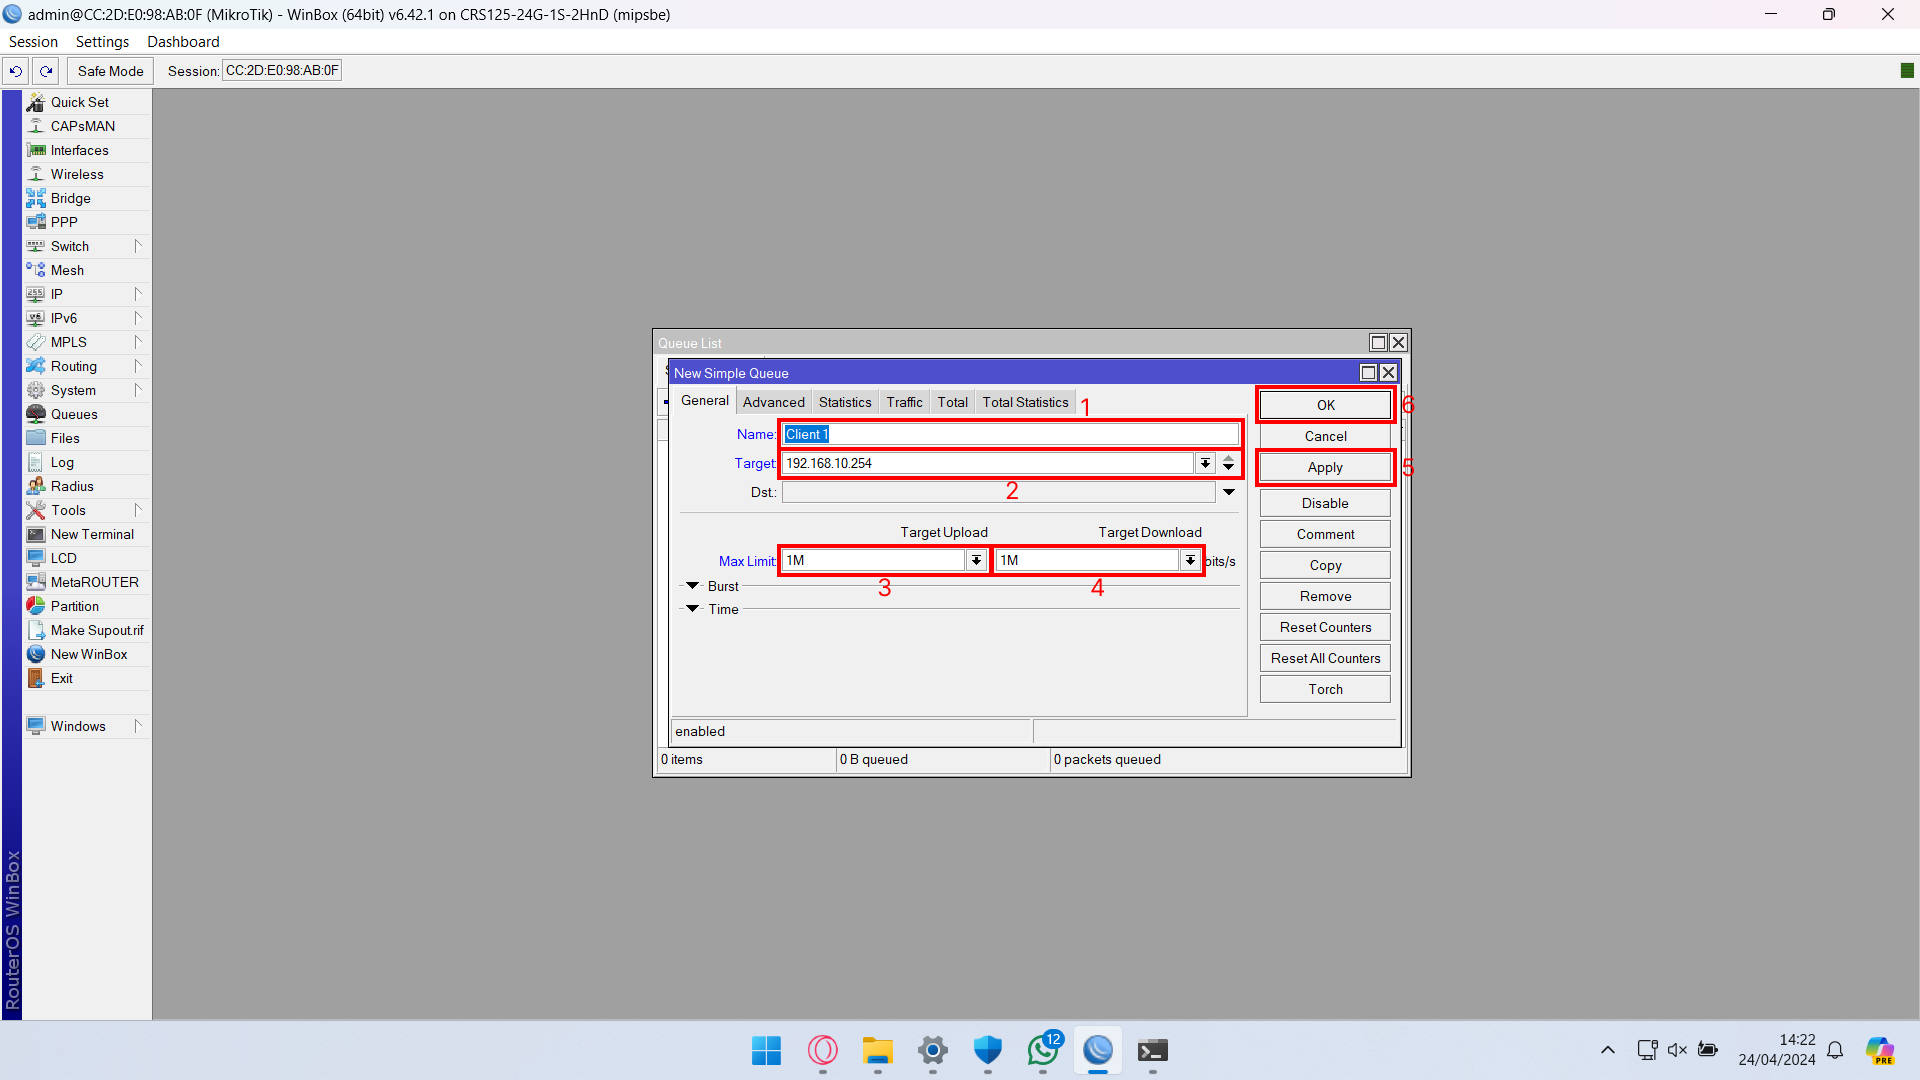
\includegraphics[width=0.8\linewidth]{P3/img/Step 18.png}
			\caption{Step 16.2}
			\label{fig:Step 16.2}
		\end{figure}
        \item Lakukan test bandwidth kembali menggunakan SPEEDTEST melalui search engine PC.
        \begin{figure}[H]
			\centering
			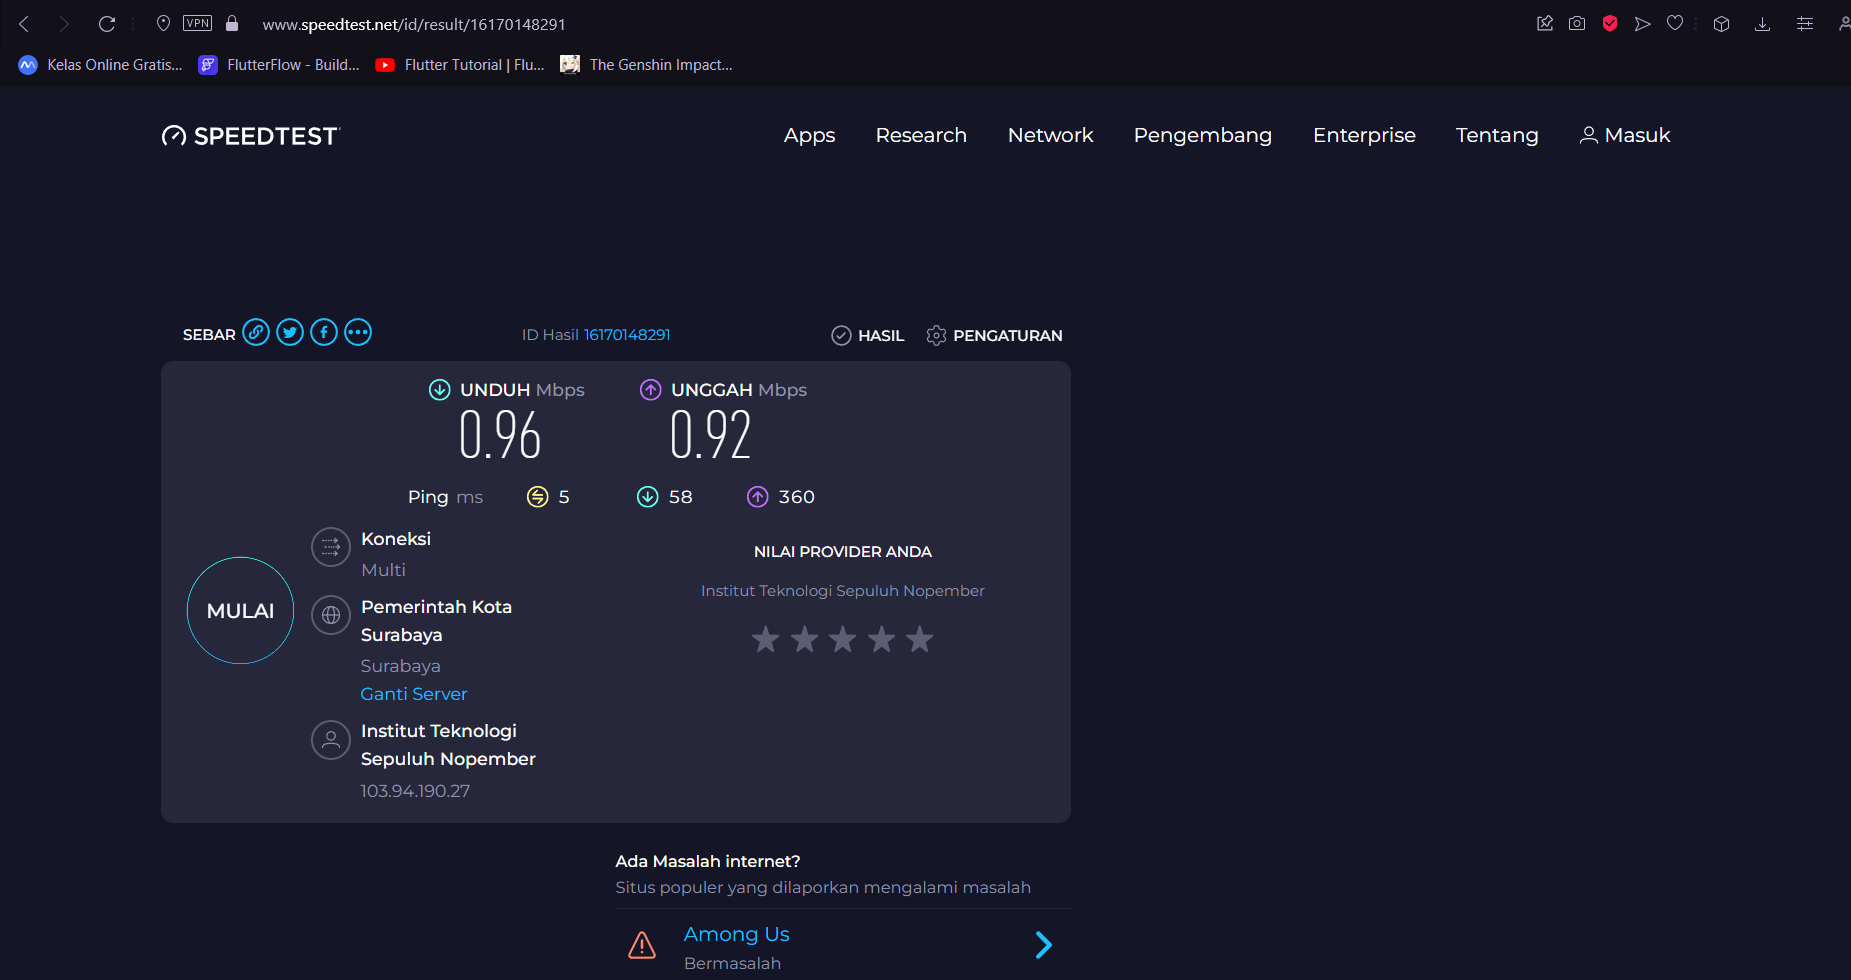
\includegraphics[width=0.8\linewidth]{P3/img/Step 19.png}
			\caption{Step 17}
			\label{fig:Step 17}
		\end{figure}
    \end{enumerate}
\end{center}

%===========================================================%
\section{Hasil yang didapat}
Memahami dan mengkonfigurasi routing dinamis RIP dengan tepat.

%===========================================================%
\section{Kesimpulan}
Dalam mengkonfigurasi routing RIP, diperlukan pemahaman dasar mengenai setting IP Address dan Subnetting, dan juga diperlukan ketelitian dan fokus agar berhasil

  \section{Pendahuluan}
\subsection{Latar Belakang}
Digital filter adalah suatu alat yang digunakan untuk memodifikasi sinyal digital dengan cara menghilangkan atau mengurangi noise, menghilangkan komponen frekuensi tertentu, dan memperbaiki kualitas sinyal. 
Digital filter sangat penting dalam berbagai aplikasi, seperti pengolahan sinyal audio, pengukuran, dan sistem monitoring.
\\\\
Ada dua jenis utama digital filter: Filter Infinite Impulse Response (IIR) dan Filter Finite Impulse Response (FIR).
Filter IIR: Menggunakan konsep feedback dan feed forward untuk menghasilkan output yang berdasarkan input sekarang, input sebelumnya, dan output sebelumnya. Filter IIR dapat memiliki respon frekuensi yang lebih kompleks dan dapat digunakan untuk aplikasi yang memerlukan pengurangan noise yang lebih efektif.
Filter FIR: Menggunakan koefisien yang ditetapkan secara eksplisit untuk menghasilkan output yang berdasarkan input sekarang saja. Filter FIR memiliki respon frekuensi yang lebih sederhana dan lebih mudah untuk dirancang, tetapi dapat lebih efektif dalam menghilangkan noise yang memiliki frekuensi tertentu.
\\\\
Dalam sistem monitoring, digital filter digunakan untuk menghilangkan noise dan memperbaiki kualitas data sensor. 
Misalnya, dalam pengukuran suhu, digital filter digunakan untuk menghilangkan noise yang dapat mempengaruhi akurasi pengukuran suhu. 

\subsection{Maksud dan Tujuan}
Memahami konsep dan aplikasi digital filter pada pengolahan sinyal digital.
\subsection{Hasil yang diharapkan}
Memahami hasil sinyal sebelum dan sesudah dilakukan digital filter.

%===========================================================%
\section{Tugas Pendahuluan}
\begin{center}
	\colorbox{cyan!30}{\parbox{0.8\linewidth}{
    \begin{enumerate}
        \item Apa itu PPTP dan bagaimana cara kerjanya?
        \item Apa kelebihan dan kekurangan dari penggunaan PPTP dibandingkan protokol VPN lainnya seperti L2TP atau OpenVPN?
    \end{enumerate}}}
\end{center}

%===========================================================%
\section{Alat dan Bahan}
\begin{itemize}[label=$\bullet$, itemsep=-1pt, leftmargin=*]
	\item 2 buah Cloud Core Router
	\item 3 Kabel UTP (LAN)
	\item 2 buah Laptop
	\item Software Winbox
\end{itemize}

%===========================================================%
\section{Jangka Waktu Pelaksanaan}
Pemahaman dan konfigurasi 1 jam.

%===========================================================%
\section{Penjelasan dan Tahapan Konfigurasi}

%======================PERCOBAAN 1==========================%
\begin{center}
    \textbf{Konfigurasi PC 1}
    \begin{enumerate}
        \item Buka aplikasi Winbox pada PC dan lakukan hubungkan ke Router. Pastikan Login terisi “admin”, Klik Neighbors > Klik Refresh > Pilih Router yang ingin disambungkan > Klik Connect.
        \begin{figure}[H]
			\centering
			\includegraphics[width=0.5\linewidth]{P4/img/pc1/Step 1.png}
			\caption{Step 1}
			\label{fig:Step 1(PC 1)}
		\end{figure}
        \item Jadikan Router menjadi DHCP Client agar bisa mendapat IP address dari Internet ITS. IP > Klik DHCP Client > Tambahkan DHCP Client > Pilih interface yang terhubung dengan Internet (ether2)> Klik Apply > Klik OK. Kita bisa memastikan koneksi ke internet dengan cara melakukan tes ping ke alamat IP 8.8.8.8
        \begin{figure}[H]
			\centering
			\includegraphics[width=0.5\linewidth]{P4/img/pc1/Step 2.1.png}
			\caption{Step 2.1}
			\label{fig:Step 2.1(PC 1)}
        \end{figure}
        \begin{figure}[H]
			\centering
			\includegraphics[width=0.8\linewidth]{P4/img/pc1/Step 2.2.png}
			\caption{Step 2.2}
			\label{fig:Step 2.2(PC 1)}
		\end{figure}
        \item Buat IP address baru pada Router 1 untuk menghubungkan PC 1 dengan Router 1. Tambahkan IP address > Isi address > Pilih Interface yang terhubung ke PC (ether4) > Klik Apply > Klik OK.
        \begin{figure}[H]
			\centering
			\includegraphics[width=0.8\linewidth]{P4/img/pc1/Step 3.png}
			\caption{Step 3}
			\label{fig:Step 3(PC 1)}
		\end{figure}
        \item Atur IP pada PC 1 dengan mengubah pengaturan pada setting ethernet. Ubah IP perangkat yang otomatis menjadi manual, pastikan IP PC 1 masih satu jaringan dengan IP lokal yang diinginkan, isi Gateway dengan IP address Router 1 yang tersambung dengan PC 1. Berikan IP address yang berbeda dengan contoh yang ada di modul.
        \begin{figure}[H]
			\centering
			\includegraphics[width=0.8\linewidth]{P4/img/pc1/Step 4.png}
			\caption{Step 4}
			\label{fig:Step 4(PC 1)}
		\end{figure}
        \item Lakukan tes ping antara Router dengan PC1, untuk memastikan PC1 dan Router sudah terkoneksi.
        \begin{figure}[H]
			\centering
			\includegraphics[width=0.8\linewidth]{P4/img/pc1/Step 5.png}
			\caption{Step 5}
			\label{fig:Step 5(PC 1)}
		\end{figure}
        \item Buat PPTP Server pada tab interface, dengan Default Profile “default -encryption”.
        \begin{figure}[H]
			\centering
			\includegraphics[width=0.8\linewidth]{P4/img/pc1/Step 6.png}
			\caption{Step 6}
			\label{fig:Step 6(PC 1)}
		\end{figure}
        \item Buat PPTP untuk client pada tab Secret, dengan konfigurasi Nama “PPTP”, Password “123456”, Service “pptp”, Profile “default”. Local Address adalah IP address tunnel pada sisi server, diisi dengan “10.10.10.2”. Remote Address adalah IP yang akan Client dapatkan, diisi dengan “10.10.10.3”. Pastikan Local Address dan Remote Address berada pada satu jaringan yang sama.
        \begin{figure}[H]
			\centering
			\includegraphics[width=0.8\linewidth]{P4/img/pc1/Step 7.png}
			\caption{Step 7}
			\label{fig:Step 7(PC 1)}
		\end{figure}
        \item Lakukan routing statis untuk menghubungkan PC1 dengan Internet. Buka pada tab IP > Routes, lalu tambahkan jaringan. Masukkan alamat jaringan yang ingin dituju, melalui alamat Gateway pada router 1
        \begin{figure}[H]
			\centering
			\includegraphics[width=0.8\linewidth]{P4/img/pc1/Step 8.png}
			\caption{Step 8}
			\label{fig:Step 8(PC 1)}
		\end{figure}
		\item Agar PC yang berada pada jaringan lokal dapat terhubung ke jaringan publik, dapat digunakan layanan NAT (Network Address Translation) yang akan menerjemahkan IP lokal beserta port perangkat agar dapat terhubung dengan jaringan publik. IP > Klik Firewall.
        \begin{figure}[H]
			\centering
			\includegraphics[width=0.8\linewidth]{P4/img/pc1/Step 16.png}
			\caption{Step 9}
			\label{fig:Step 9(PC 1)}
		\end{figure}
		\item Buat NAT baru. Klik tab NAT > Tambahkan NAT > Pada Opsi Chain pilih srcnat > Pilih Out Interface yaitu port pada Router yang terhubung dengan Internet(ether6) > Klik Apply. Tambahkan Action pada tab Action. Pada Opsi Action pilih masquerade > Klik Apply > Klik OK.
        \begin{figure}[H]
			\centering
			\includegraphics[width=0.5\linewidth]{P4/img/pc1/Step 15.png}
			\caption{Step 10.1}
			\label{fig:Step 10.1(PC 1)}
        \end{figure}
        \begin{figure}[H]
			\centering
			\includegraphics[width=0.8\linewidth]{P4/img/pc1/Step 14.png}
			\caption{Step 10.2}
			\label{fig:Step 10.2(PC 1)}
		\end{figure}	
    \end{enumerate}
	\textbf{Pengujian Konfigurasi}
	\begin{enumerate}
		\item Lakukan tes ping ke alamat Remote Address Router 2 untuk memastikan kedua Router sudah terhubung.
		\begin{figure}[H]
			\centering
			\includegraphics[width=0.8\linewidth]{P4/img/pc1/Step 9.png}
			\caption{Step 1}
			\label{fig:Ping Step 1(PC 1)}
		\end{figure}
		\item Lakukan tes ping ke PC 2 untuk memastikan kedua PC sudah terhubung.
		\begin{figure}[H]
			\centering
			\includegraphics[width=0.8\linewidth]{P4/img/pc1/Step 10.png}
			\caption{Step 2}
			\label{fig:Ping Step 2(PC 1)}
		\end{figure}
	\end{enumerate}

    \textbf{Konfigurasi PC 2}
    \begin{enumerate}
        \item Hubungkan PC2 dengan Internet, bisa dilakukan menggunakan wifi ITS.
        \begin{figure}[H]
			\centering
			\includegraphics[width=0.5\linewidth]{P4/img/pc2/Step 1.png}
			\caption{Step 1}
			\label{fig:Step 1(PC 2)}
		\end{figure}
        \item Cek IP yang diterima PC2 dari ITS.
        \begin{figure}[H]
			\centering
			\includegraphics[width=0.5\linewidth]{P4/img/pc2/Step 2.png}
			\caption{Step 2}
			\label{fig:Step 2(PC 2)}
        \end{figure}
        \item Masuk ke dalam setting PC2 dan klik VPN.
        \begin{figure}[H]
			\centering
			\includegraphics[width=0.8\linewidth]{P4/img/pc2/Step 3.png}
			\caption{Step 3}
			\label{fig:Step 3(PC 2)}
		\end{figure}
        \item Hubungkan client PPTP dengan server PPTP, untuk melakukan hal tersebut, buatlah koneksi VPN baru antara PC2 dengan Host Server. Pastikan menggunakan VPN type PPTP. Pastikan Username dan password sudah sesuai dengan konfigurasi Router1.
        \begin{figure}[H]
			\centering
			\includegraphics[width=0.8\linewidth]{P4/img/pc2/Step 4.png}
			\caption{Step 4}
			\label{fig:Step 4(PC 2)}
		\end{figure}
        \item Hubungkan ke VPN dengan cara klik tombol Connect
        \begin{figure}[H]
			\centering
			\includegraphics[width=0.8\linewidth]{P4/img/pc2/Step 5.png}
			\caption{Step 5}
			\label{fig:Step 5(PC 2)}
		\end{figure}
    \end{enumerate}

	\textbf{Pengujian Konfigurasi}
	\begin{enumerate}
		\item Lakukan tes ping ke alamat PC1 untuk memastikan VPN PPTP sudah terhubung.
		\begin{figure}[H]
			\centering
			\includegraphics[width=0.8\linewidth]{P4/img/pc2/Step 6.png}
			\caption{Step 1}
			\label{fig:Ping Step 1(PC 2)}
		\end{figure}
	\end{enumerate}
\end{center}

%===========================================================%
\section{Hasil yang didapat}
Memahami penerapan dan penghubungan jaringan dengan menerapkan PPTP dengan VPN

%===========================================================%
\section{Kesimpulan}
Dalam mengkonfigurasi VPN, diperlukan pemahaman dasar mengenai metode PPTP, dan juga diperlukan ketelitian dan fokus agar berhasil

% \section{Pendahuluan}
\subsection{Latar Belakang}
modul ini dipengaruhi ...

\subsection{Maksud dan Tujuan}
\begin{center}
    \begin{enumerate}
        \item Mengetahui bagaimana konfigurasi static routing menggunakan Ipv6
        \item Mengimplementasikan konfigurasi Ipv6 pada perangkat mikrotik
    \end{enumerate}
\end{center}

%===========================================================%
\section{Tugas Pendahuluan}
\begin{center}
	\colorbox{cyan!30}{\parbox{0.8\linewidth}{
    \begin{enumerate}
        \item Apa solusi lain ketika IPv4 habis, selain menggunakan IPv6?
        \item Sebutkan tiga keunggulan IPv6 dibandingkan IPv4!
        \item Mengapa panjang awal alamat IPv6 biasanya adalah 128 bit?
    \end{enumerate}}}
\end{center}

%===========================================================%
\section{Alat dan Bahan}
\begin{itemize}[label=$\bullet$, itemsep=-1pt, leftmargin=*]
	\item 2 buah Cloud Core Router
	\item 3 Kabel UTP (LAN)
	\item 2 buah Laptop
	\item Software Winbox
\end{itemize}

%===========================================================%
\section{Jangka Waktu Pelaksanaan}
Pemahaman dan konfigurasi 1 jam.

%===========================================================%
\section{Penjelasan dan Tahapan Konfigurasi}

%======================PERCOBAAN 1==========================%
\begin{center}
    \textbf{Konfigurasi PC 1}
    \begin{enumerate}

        \item Buka aplikasi Winbox pada PC1 dan hubungkan ke Router. Pastikan Login terisi “admin”, Klik Neighbors > Klik Refresh > Pilih Router yang ingin disambungkan > Klik Connect.
        \begin{figure}[H]
			\centering
			\includegraphics[width=0.5\linewidth]{P5/img/pc1/Step 1.png}
			\caption{Step 1}
			\label{fig:Step 1(PC 1)}
		\end{figure}

        \item Konfigurasikan Router1 untuk mengaktifkan layanan IPv6. Klik System > Klik Packages > Klik IPv6 > Klik Enable > Reboot ulang Router1.
        \begin{figure}[H]
			\centering
			\includegraphics[width=0.5\linewidth]{P5/img/pc1/Step 2.png}
			\caption{Step 2}
			\label{fig:Step 2(PC 1)}
        \end{figure}

        \item Konfigurasi IPv6 Router 1 untuk menghubungkan PC 1 dengan Router 1. Tambahkan IP address > Isi address > pilih Interface yang terhubung ke PC 1 atau ether4 > Klik Apply > Klik OK.
        \begin{figure}[H]
			\centering
			\includegraphics[width=0.8\linewidth]{P5/img/pc1/Step 3.png}
			\caption{Step 3}
			\label{fig:Step 3(PC 1)}
		\end{figure}

        \item Konfigurasi IPv6 pada PC 1 dengan mengubah pengaturan pada setting ethernet. Ubah IPv6 perangkat yang otomatis menjadi manual, pastikan IPv6 PC 1 masih satu jaringan dengan IPv6 lokal yang diinginkan, isi Gateway dengan IPv6 address Router 1 yang tersambung dengan PC 1. Berikan IPv6 address yang berbeda dengan contoh yang ada di modul.
        \begin{figure}[H]
			\centering
			\includegraphics[width=0.8\linewidth]{P5/img/pc1/Step 4.png}
			\caption{Step 4}
			\label{fig:Step 4(PC 1)}
		\end{figure}

        \item Lakukan uji coba ping dari Router 1 ke PC 1 dan sebaliknya untuk memastikan kedua perangkat sudah saling terhubung.
        \begin{figure}[H]
			\centering
			\includegraphics[width=0.8\linewidth]{P5/img/pc1/Step 5.png}
			\caption{Step 5}
			\label{fig:Step 5(PC 1)}
		\end{figure}

        \item Konfigurasi IPv6 Router 1 untuk menghubungkan Router 1 dengan Router 2. Tambahkan address IPv6 > Isi address > pilih Interface yang terhubung ke Router 2 (ether2) > Klik Apply > Klik OK.
        \begin{figure}[H]
			\centering
			\includegraphics[width=0.8\linewidth]{P5/img/pc1/Step 6.png}
			\caption{Step 6}
			\label{fig:Step 6(PC 1)}
		\end{figure}

        \item Hubungkan kedua Network menggunakan routing statis. Buka pada tab IPv6 > Routes. Lalu tambahkan routes. Masukkan alamat jaringan yang ingin dituju, melalui alamat Gateway pada Router 2.
        \begin{figure}[H]
			\centering
			\includegraphics[width=0.8\linewidth]{P5/img/pc1/Step 7.png}
			\caption{Step 7}
			\label{fig:Step 7(PC 1)}
		\end{figure}
    \end{enumerate}

    \textbf{Konfigurasi PC 2}
    \begin{enumerate}
        \item Buka aplikasi Winbox pada PC2 dan hubungkan ke Router. Pastikan Login terisi “admin”, Klik Neighbors > Klik Refresh > Pilih Router yang ingin disambungkan > Klik Connect.
        \begin{figure}[H]
			\centering
			\includegraphics[width=0.5\linewidth]{P5/img/pc2/Step 1.png}
			\caption{Step 1}
			\label{fig:Step 1(PC 2)}
		\end{figure}
        \item Konfigurasikan Router2 untuk mengaktifkan layanan IPv6. Klik System > Klik Packages > Klik IPv6 > Klik Enable > Reboot ulang Router2.
        \begin{figure}[H]
			\centering
			\includegraphics[width=0.5\linewidth]{P5/img/pc2/Step 2.png}
			\caption{Step 2}
			\label{fig:Step 2(PC 2)}
        \end{figure}
        \item Konfigurasi IPv6 Router 2 untuk menghubungkan PC 2 dengan Router 2. Tambahkan IP address > Isi address > pilih Interface yang terhubung ke PC 2 (ether4) > Klik Apply > Klik OK.
        \begin{figure}[H]
			\centering
			\includegraphics[width=0.8\linewidth]{P5/img/pc2/Step 3.png}
			\caption{Step 3}
			\label{fig:Step 3(PC 2)}
		\end{figure}
        \item Konfigurasi IPv6 pada PC 2 dengan mengubah pengaturan pada setting ethernet. Ubah IPv6 perangkat yang otomatis menjadi manual, pastikan IPv6 PC 2 masih satu jaringan dengan IPv6 lokal yang diinginkan, isi Gateway dengan IPv6 address Router 2 yang tersambung dengan PC 2. Berikan IPv6 address yang berbeda dengan contoh yang ada di modul.
        \begin{figure}[H]
			\centering
			\includegraphics[width=0.8\linewidth]{P5/img/pc2/Step 4.png}
			\caption{Step 4}
			\label{fig:Step 4(PC 2)}
		\end{figure}
        \item Lakukan uji coba ping dari Router 2 ke PC 2 dan sebaliknya untuk memastikan kedua perangkat sudah saling terhubung.
        \begin{figure}[H]
			\centering
			\includegraphics[width=0.8\linewidth]{P5/img/pc2/Step 5.png}
			\caption{Step 5}
			\label{fig:Step 5(PC 2)}
		\end{figure}
    
        \item Konfigurasi IPv6 Router 2 untuk menghubungkan Router 2 dengan Router 1. Tambahkan address IPv6 > Isi address > pilih Interface yang terhubung ke Router 1 (ether2) > Klik Apply > Klik OK.
        \begin{figure}[H]
			\centering
			\includegraphics[width=0.8\linewidth]{P5/img/pc2/Step 6.png}
			\caption{Step 6}
			\label{fig:Step 6(PC 2)}
		\end{figure}
        \item Hubungkan kedua Network menggunakan routing statis. Buka pada tab IPv6 > Routes. Lalu tambahkan routes. Masukkan alamat jaringan yang ingin dituju, melalui alamat Gateway pada Router 1.
        \begin{figure}[H]
			\centering
			\includegraphics[width=0.8\linewidth]{P5/img/pc2/Step 7.png}
			\caption{Step 7}
			\label{fig:Step 7(PC 2)}
		\end{figure}
    \end{enumerate}

	\textbf{Pengujian Konfigurasi}
	\begin{enumerate}
		\item Lakukan tes ping ke alamat IPv6 PC 2 untuk memastikan kedua PC sudah terhubung.
		\begin{figure}[H]
			\centering
			\includegraphics[width=0.8\linewidth]{P5/img/pc1/Step 8.png}
			\caption{Step 1}
			\label{fig:Ping Step 1}
		\end{figure}
        \item Lakukan tes ping ke alamat IPv6 PC 1 untuk memastikan kedua PC sudah terhubung.
		\begin{figure}[H]
			\centering
			\includegraphics[width=0.8\linewidth]{P5/img/pc2/Step 8.png}
			\caption{Step 2}
			\label{fig:Ping Step 2}
		\end{figure}
	\end{enumerate}

\end{center}

%===========================================================%
\section{Hasil yang didapat}
Memahami penerapan dan penghubungan jaringan dengan menerapkan IPv6 pada konfigurasi statis

%===========================================================%
\section{Kesimpulan}
Dalam mengkonfigurasi IPv6, diperlukan pemahaman dasar mengenai penghubungan jaringan dengan menggunakan konfigurasi statis



\renewcommand\refname{Daftar Pustaka} % Menghilangkan kata "Daftar Pustaka"
\renewcommand{\bibname}{} % Menghilangkan kata "Bibliography"

\printbibliography
\end{document}